\documentclass[11pt,a4paper]{article}

\usepackage[margin=2.5cm]{geometry}
\usepackage{amsmath,amssymb,amsthm}
\usepackage{mathtools}
\usepackage{booktabs}
\usepackage{tikz}
\usepackage{pgfplots}
\pgfplotsset{compat=1.18}
\usepackage[hidelinks]{hyperref}
\usepackage{enumitem}

\newtheorem{theorem}{Theorem}[section]
\newtheorem{lemma}[theorem]{Lemma}
\newtheorem{proposition}[theorem]{Proposition}
\newtheorem{corollary}[theorem]{Corollary}
\newtheorem{definition}[theorem]{Definition}
\newtheorem{remark}[theorem]{Remark}
\newtheorem{convention}[theorem]{Convention}
\newtheorem{example}[theorem]{Example}
\newtheorem{conjecture}[theorem]{Conjecture}

\newcommand{\Lin}{\mathrm{L}}
\newcommand{\Herm}{\mathrm{Herm}}
\newcommand{\Sstate}{\mathcal{S}}
\newcommand{\Chan}{\mathrm{Chan}}
\newcommand{\Inst}{\mathrm{Inst}}
\newcommand{\RepInst}{\mathrm{RepInst}}
\newcommand{\Tr}{\operatorname{Tr}}
\newcommand{\id}{\operatorname{id}}
\newcommand{\supp}{\operatorname{supp}}
\newcommand{\rank}{\operatorname{rank}}
\newcommand{\diam}{\operatorname{diam}}
\newcommand{\coind}{\operatorname{coind}_{\mathbb Z_2}}
\newcommand{\Jhat}{\widehat J}
\newcommand{\vD}{\vec{\Delta}}
\newcommand{\aff}{\operatorname{aff}}

\title{\bf Exact Affine Geometry, Optimal Centres, Certified Compression Bounds, and Flag-Quotient Width Obstructions for Finite-Outcome Quantum Instruments}
\author{Amin Abaee\\
\small Independent Researcher\\
\small ORCID: 0000-0002-0019-1842\\
\small Email: \href{mailto:amin\_abaee@ut.ac.ir}{amin\_abaee@ut.ac.ir}}
\date{September 14, 2026}

\begin{document}
\maketitle

\begin{abstract}
Quantum instruments describe the full statistics of a measurement together with the conditional post-measurement state, and they form the building blocks of adaptive protocols and quantum networks. We study the geometry of the set of all $n$-outcome instruments acting between two finite-dimensional quantum systems, and we ask how many continuous real parameters must be retained in order to encode an arbitrary instrument and later reconstruct it with uniformly small error, under the convention of continuous encoding and unrestricted decoding. The geometry of the instrument body is determined exactly: its affine dimension is $d_A^2(nd_B^2-1)$; the largest diamond-norm ball contained in the body has radius $2/(nd_B\min\{d_A,d_B\})$ and is centred at the uniform depolarising instrument, which is optimal among all centres; and the same instrument is optimal for the covering problem, with an exact covering radius linked to the in-radius by a complementarity identity. Every radius and width carries a single-shot operational meaning through the optimal discrimination error. On the compression side, antipodal constructions --- output preparation, an input-dependent observable sphere, and a full-direction section --- produce a certified lower envelope on the optimal error; constructive upper bounds from constant codes, convex projection, and balanced pinching meet the envelope exactly at zero latent dimension (where both equal the exact constant-code width), in the collapse case, and from the affine dimension on, and bracket it in the intermediate regime; the zero-error threshold equals the affine dimension. For the input-independent case the flat-width classification is complete: the flat value one holds exactly on the classical $n\le4$ and qubit $n\le2$ bodies and fails at least $4/3$ on every other, including every state space of dimension $\ge3$ at the bottom and second latent dimensions alike, the qutrit exactly $4/3$ at both, the second-index result resting on the integral cohomology of the cyclic flag quotient. The single-outcome case recovers quantum channels, and the one-dimensional-output case recovers finite-outcome measurements; the trade-off between the number of outcomes and the robustness of the uniform instrument is made explicit.
\end{abstract}

\noindent\textbf{Keywords:} quantum instruments; diamond norm; compression width; Chebyshev radius; equivariant cohomology; Borsuk--Ulam theorem.

\section{Introduction}
\label{sec:intro}

Quantum instruments are the natural generalisation of quantum channels to finite-outcome statistics: a collection of completely positive, trace-nonincreasing maps whose sum is a channel. They describe both the probability of an outcome and the conditional post-measurement state, and they model finite-outcome measurements, adaptive protocols, and the nodes of quantum networks~\cite{DaviesLewis1970,Ozawa1984,ChiribellaEtAl2009Instruments,ChiribellaEtAl2008Combs}.

The general source--latent theory underlying the obstruction arguments --- fiber radii, antipodal profiles, deleted-product coindex, and stable Lipschitz variants --- is developed for channels in Ref.~\cite{CompanionChannels}; the present paper uses the specialisations recorded in Sections~\ref{sec:lower} and~\ref{sec:widths}. Throughout, the $n=1$ restrictions of the instrument theorems below recover the corresponding channel-level statements of~\cite{CompanionChannels}: the observable sphere, the full-direction sphere, the join, the global in-radius, and the covering results.

The question treated here is the instrument-level analogue of the channel problem: does the compact convex body of $n$-outcome instruments between $A$ and $B$ admit a continuous low-dimensional latent encoding with uniformly accurate decoding? Throughout, we adopt the standard asymmetric convention: the \emph{encoder is continuous} and the \emph{decoder is unrestricted} (Convention~\ref{conv:decoder}); where a continuous decoder is additionally available we say so explicitly. The answer has three regimes. At small latent dimension, input-independent preparation of a flagged output state already forces error one. In an intermediate range, the width is bracketed between a certified lower and a certified upper envelope: a centred-ball bound scaling as $1/n$ --- which Theorem~\ref{thm:global-inradius} shows is the best centred-ball certificate at any centre --- plus a full-direction antipodal obstruction contributing an $n$-independent component $1/d_A$, against upper bounds that never sink below one. From the affine dimension on, exact reconstruction holds, even with a continuous decoder.

The main contribution of this paper is the exact affine geometry of the instrument body and its compression consequences: the affine dimension, the centred and global in-radii, the covering radius, and the diameter are determined exactly, with the uniform depolarising instrument turning out to be an optimal centre simultaneously for the in-radius and the covering radius (a concave--convex duality, Theorem~\ref{thm:global-inradius} and Remark~\ref{rem:duality}). Which quantities are determined \emph{exactly}, and which only by \emph{certified bounds}, is stated once in Remark~\ref{rem:exact-vs-certified} and maintained throughout. A separate physical question --- whether an abstract code can be realised by a fixed programmable processor --- is addressed in Appendix~\ref{app:no-programming}: exact finite-dimensional evaluation of all unitary channels is impossible, and vanishing error forces unbounded program dimension. This separates \emph{representational} dimension from \emph{programmable} evaluation; the main theorems do not rely on the appendix. For the input-independent case $d_A=1$, the flat-width problem is governed by the flag-coordinate count $nd_B$: the antipodal floor $1$ is exact precisely on the upper side $nd_B\le2r+2$ of the subcritical range for classical and qubit outputs, and the width is bounded away from $1$ on the lower side $nd_B\ge2r+3$ --- at least $4/3$, with the exact boundary value $4/3$ and the exact value $2(1-1/d_B)$ at latent dimension $n-1$ for prime-power output dimensions; and the bottom width is classified completely --- flat exactly on the classical $n\le4$ and qubit $n\le2$ bodies, at least $4/3$ on every other input-independent body, including every state space of dimension $\ge3$, with the qutrit state space exactly at $4/3$, and the second latent dimension of every such state space likewise bounded below by $4/3$, exactly $4/3$ at the qutrit --- the latter through a Chern-transgression derivation of the integral cohomology of the cyclic flag quotient, cross-checked by an independent exact-integer machine computation (Theorems~\ref{thm:nonflat-d1}, \ref{thm:tverberg}, \ref{thm:flat-half}, \ref{thm:flat-qubit}, \ref{thm:mass-exact}, \ref{thm:equal-basis}, \ref{thm:equal-basis-plane}, \ref{thm:state-nonflat}, \ref{thm:state-d2}; Corollaries~\ref{cor:exact-d1} and~\ref{cor:bottom-dichotomy}). The cohomological premise entering through Lemma~\ref{lem:flag-cohomology} sits next to an active literature on the cohomology of unordered flag quotients, Auerbach bases, and cyclic-group Borsuk--Ulam theorems; Remark~\ref{rem:flag-literature} records the precise differentiation.

The paper is organised as follows. Section~\ref{sec:prelim} fixes notation and conventions; the specialised forms of the source--latent theory of Ref.~\cite{CompanionChannels} are recorded where they are used, in Sections~\ref{sec:lower} and~\ref{sec:widths}. Section~\ref{sec:exact-geometry} determines the exact affine and metric parameters of the instrument body, and Section~\ref{sec:lower} constructs the antipodal certificates and the certified lower envelope. Section~\ref{sec:widths} develops the constructive upper bounds and the exact thresholds, and Section~\ref{sec:specialisations} collects the specialisations, worked examples, and the outcome trade-off. Section~\ref{sec:conclusion} summarises which quantities are exact and which are certified and lists the open problems; Appendix~\ref{app:no-programming} records the no-programming background.

\section{Preliminaries}
\label{sec:prelim}

Throughout, $A$ and $B$ are finite-dimensional Hilbert spaces of dimensions $d_A,d_B$, and $n\in\mathbb N$ is the number of outcomes. Let $A_0\simeq A$ be a reference copy with a fixed pair of conjugate bases in $A_0$ and $A$, and define the maximally entangled state
\[
|\omega_A\rangle=\frac1{\sqrt{d_A}}\sum_{j=1}^{d_A}|j\rangle_{A_0}|j\rangle_A.
\]
For a map $\Phi:\Lin(A)\to\Lin(B)$ the \emph{normalised Choi operator} is
\[
\Jhat_\Phi=(\id_{A_0}\otimes\Phi)(|\omega_A\rangle\langle\omega_A|),
\]
the Choi--Jamio{\l}kowski isomorphism in the normalised form~\cite{Choi1975,Jamiolkowski1972}.

\begin{remark}[Normalised Choi convention]
\label{rem:choi-convention}
With the unnormalised maximally entangled vector $|\Omega_A\rangle=\sum_j|j\rangle_{A_0}|j\rangle_A$ one has $\Jhat_\Phi=\tfrac1{d_A}J_\Phi^{\mathrm{unnorm}}$. Consequently $\Phi$ is trace preserving if and only if
\[
\Tr_B\Jhat_\Phi=\frac{I_{A_0}}{d_A}.
\]
All affine constraints, radii, covering bounds, and pinching dimension counts in this paper use this normalised convention.
\end{remark}

Let $C_n$ be an $n$-dimensional classical flag space with basis $|1\rangle,\dots,|n\rangle$.

\begin{definition}[Instrument, flagged channel, and instrument diamond norm]
An $n$-outcome instrument from $A$ to $B$ is a tuple $\mathcal I=(\mathcal I_1,\dots,\mathcal I_n)$ of completely positive, trace-nonincreasing maps whose sum is a channel. Write $\Inst_n(A,B)$ for the set of all such instruments. The flagged channel of $\mathcal I$ is
\[
\widehat{\mathcal I}(X)=\sum_{k=1}^n\mathcal I_k(X)\otimes|k\rangle\langle k|.
\]
For a tuple $\vD=(\Delta_1,\dots,\Delta_n)$ of Hermiticity-preserving maps, define the flagged map and the instrument diamond norm by
\[
\widehat{\vD}(X)=\sum_{k=1}^n\Delta_k(X)\otimes|k\rangle\langle k|,
\qquad
\|\vD\|_{\diamond,\mathrm{inst}}=\|\widehat{\vD}\|_\diamond.
\]
By block diagonality (the trace norm of a block-diagonal operator is the sum of the trace norms of its blocks) this equals the operational formula
\[
\|\vD\|_{\diamond,\mathrm{inst}}
=\sup_{\rho\in\Sstate(A_0\otimes A)}
\sum_{k=1}^n\|(\id_{A_0}\otimes\Delta_k)(\rho)\|_1.
\]
The diamond norm was introduced in~\cite{AharonovKitaevNisan1998}; a reference system of input dimension $d_A$ suffices for it~\cite{Watrous2018}. The summands are the unconditional, generally subnormalised outcome contributions. The body $\Inst_n(A,B)$ is compact and convex: convexity follows from the convexity of the completely positive cone and the affine normalisation constraints, and compactness from positivity together with the summed marginal condition, which bounds every Choi block.
\end{definition}

\begin{remark}[Operational meaning]
\label{rem:operational}
For two instruments $\mathcal I,\mathcal J$ with equal prior probabilities, the optimal single-use discrimination success probability, with arbitrary reference assistance, is
\[
p_{\mathrm{succ}}
=\frac12+\frac14\,\|\mathcal I-\mathcal J\|_{\diamond,\mathrm{inst}},
\]
i.e.\ the advantage over random guessing is $\tfrac14\|\mathcal I-\mathcal J\|_{\diamond,\mathrm{inst}}$ (an instance of the Holevo--Helstrom theorem for binary state discrimination~\cite{Helstrom1976}, applied to the flagged outputs). Thus every radius and width stated in the instrument diamond norm has a direct single-shot discrimination interpretation, up to this conventional factor of $1/4$.
\end{remark}

The ambient affine space and its direction space are
\begin{align*}
\mathfrak A_{A,B}^{(n)}
&=\Big\{(\Phi_1,\dots,\Phi_n):
\Phi_k\ \text{Hermiticity-preserving},\quad
\sum_{k=1}^n\Tr_B\Jhat_{\Phi_k}=\frac{I_{A_0}}{d_A}\Big\},\\
\mathfrak V_{A,B}^{(n)}
&=\Big\{(\Delta_1,\dots,\Delta_n):
\Delta_k\ \text{Hermiticity-preserving},\quad
\sum_{k=1}^n\Tr_B\Jhat_{\Delta_k}=0\Big\}.
\end{align*}
Here $\mathfrak V_{A,B}^{(n)}$ is the real linear direction space, of real dimension $D_{A,B}^{(n)}$ when $nd_B>1$.
Thus only the summed direction is trace-annihilating; individual outcome components need not be. For $\mathcal I_0\in\mathfrak A_{A,B}^{(n)}$ define the closed relative instrument-diamond ball
\[
\overline B_{\diamond,\mathrm{inst}}^{\mathrm{rel}}(\mathcal I_0,\rho)
=\big\{\mathcal I_0+\vD:\vD\in\mathfrak V_{A,B}^{(n)},\ \|\vD\|_{\diamond,\mathrm{inst}}\le\rho\big\},
\]
and, for $\mathcal I_0\in\Inst_n(A,B)$, its centred relative in-radius
\[
\rho_{\diamond,\mathrm{inst}}(\mathcal I_0)
=\sup\Big\{\rho\ge0:
\overline B_{\diamond,\mathrm{inst}}^{\mathrm{rel}}(\mathcal I_0,\rho)
\subseteq\Inst_n(A,B)\Big\}.
\]
Let $\mathcal I_*$ be the uniform depolarising instrument, $(\mathcal I_*)_k=\Omega_{A,B}/n$, where $\Omega_{A,B}(X)=\Tr(X)I_B/d_B$, so that $\Jhat_{(\mathcal I_*)_k}=I_{A_0\otimes B}/(n d_Ad_B)$. The centred in-radius of the body about $\mathcal I_*$ and its covering radius, denoted $\rho_n$ and $R_n$ throughout with $s=\min\{d_A,d_B\}$, are determined exactly in Theorems~\ref{thm:exact-radius} and~\ref{thm:covering} below: $\rho_n=2/(nd_Bs)$ and $R_n=2-\rho_n$.

\begin{remark}[POVM case $d_B=1$]
\label{rem:povm}
When $d_B=1$, identify $\Lin(B)$ with $\mathbb C$. An instrument component is a positive functional $\mathcal I_k(X)=\Tr(E_kX)$ for a unique effect $E_k\ge0$, and the instrument condition is exactly $\sum_{k=1}^nE_k=I_A$. Thus $\Inst_n(A,\mathbb C)$ is the convex body of $n$-outcome POVMs on $A$.
\end{remark}

\begin{remark}[Degenerate singleton case]
\label{rem:degenerate}
If $n=d_B=1$, then $\Inst_1(A,\mathbb C)$ consists of the unique trace functional $X\mapsto\Tr(X)$: its affine dimension is $D_{A,1}^{(1)}=0$, its direction space is $\{0\}$, every compression width is $0$, and, because every relative ball is the singleton, the centred relative in-radius is $+\infty$ under the supremum convention (the formula $2/(nd_Bs)$ does not apply). Except where explicitly stated, all nontrivial statements in this paper assume
\[
n d_B>1.
\]
\end{remark}

\begin{remark}[Exact claims versus certified bounds]
\label{rem:exact-vs-certified}
The following statements are exact: (i) the affine dimension $D_{A,B}^{(n)}$; (ii) the centred in-radius at the uniform instrument; (iii) the global in-radius over all centres, which equals (ii) by Theorem~\ref{thm:global-inradius}; (iv) the global covering radius and optimality of $\mathcal I_*$ as a centre; (v) the diameter, equal to $2$; (vi) the antipodal profile of the replacement body, and hence of the full body when $d_A=1$; (vii) the constant-code width $\delta_{0,\mathrm{inst}}^{\diamond}(A,B)=R_{\mathrm{inst}}(\mathcal I_*)$, which supplies the $r=0$ value of the certified lower envelope (Definition~\ref{def:beta-best}); (viii) the zero-error Euclidean threshold for continuous encoding with unrestricted decoding; (ix) the full width function in the collapse case $nd_Bs=2$ (Theorem~\ref{thm:collapse}); (x) for $d_A=d_B=1$, the full subcritical dichotomy: $\delta_r=1$ for $n\le2r+2$, $\delta_r\ge4/3$ for $n\ge2r+3$, with the exact boundary value $\delta_r=4/3$ at $n=2r+3$ (Theorem~\ref{thm:flat-half}, Corollaries~\ref{cor:classical-dichotomy} and~\ref{cor:exact-d1}); (xi) for $d_A=1$, $d_B=2$, the full subcritical dichotomy $\delta_r=1$ for $n-1\le r\le nd_B^2-2$ and $\delta_r\ge4/3$ for $r\le n-2$ (Theorem~\ref{thm:flat-qubit}, Corollaries~\ref{cor:flat-fails} and~\ref{cor:qubit-dichotomy}); (xii) for $d_A=1$ and $d_B$ a prime power, the exact width $\delta_{n-1}=2(1-1/d_B)$, and the exact bottom width $\delta_1=4/3$ at $n=5$ (Theorem~\ref{thm:mass-exact}, Corollary~\ref{cor:exact-d1}); (xiii) for $d_A=1$, the complete bottom-width classification: $\delta_1=1$ exactly when $nd_B\le4$ and $d_B\le2$, $\delta_1\ge4/3$ otherwise, with the exact value $4/3$ at $(n,d_B)\in\{(5,1),(1,3),(2,3)\}$, the one-outcome ququart in $[4/3,3/2]$, and $\delta_1=4/3$ on every state space of dimension $\ge3$ (Theorems~\ref{thm:equal-basis}, \ref{thm:state-nonflat} and~\ref{thm:mass-exact}; Corollaries~\ref{cor:exact-d1} and~\ref{cor:bottom-dichotomy}). The following are certified bounds or open quantities, not exact determinations: (a) the intermediate compression widths $\delta_{r,\mathrm{inst}}^{\diamond}(A,B)$ for $0<r<D_{A,B}^{(n)}$ outside the input-independent flat regimes of items (x)--(xiii); (b) the full antipodal profile beyond the certified constructions; (c) optimality of the certified upper envelope $U_r^{(n)}$. Table~\ref{tab:summary} collects the complete regime-by-regime picture.
\end{remark}

\begin{remark}[Notation]
\label{rem:notation}
To avoid collisions, the following symbols are used as consistently as the subject allows: ranks are denoted $r_E$, the number of input pinching blocks by $k_{\mathrm{in}}$, the number of output pinching blocks by $\ell_{\mathrm{out}}$, the latent dimension by $r$ (or $q$ for general latent spaces), the covering radius by $R$, subspaces of input systems, flag-output systems, or supports by $W$ (the join constructions of Section~\ref{sec:lower} use $W\subseteq B\otimes C_n$ on the flag-output side), and the reference system in the covering arguments by $E$ (a copy of $A_0$, the diamond-norm reference of the definition of the instrument diamond norm); Appendix~\ref{app:no-programming} additionally uses $E$ for the programming input system, in a self-contained notation. The conjugations in Lemma~\ref{lem:spectral} and Theorem~\ref{thm:exact-radius} act on opposite factors of the reference pair; both are consistent with the fixed Choi bases and produce the same maximally entangled probes.
\end{remark}

\section{Exact affine and metric parameters}
\label{sec:exact-geometry}

This section determines the affine dimension, the centred in-radius at the uniform instrument, the global in-radius, the covering radius, and the diameter of the instrument body, all exactly.

\begin{proposition}[Affine dimension of the instrument body]
\label{prop:dimension}
Assume $nd_B>1$. Then
\[
\dim_{\mathbb R}\aff\,\Inst_n(A,B)
=D_{A,B}^{(n)}:=d_A^2(nd_B^2-1).
\]
\end{proposition}

\begin{proof}
An instrument Choi tuple consists of $n$ Hermitian operators on $A_0\otimes B$, of total real dimension $nd_A^2d_B^2$. The normalisation constraint
\[
\sum_{k=1}^n\Tr_B\Jhat_{\mathcal I_k}=\frac{I_{A_0}}{d_A}
\]
imposes $d_A^2=\dim_{\mathbb R}\Herm(A_0)$ real affine equations. The linear map $(X_1,\dots,X_n)\mapsto\sum_k\Tr_BX_k$ from $\bigoplus_k\Herm(A_0\otimes B)$ to $\Herm(A_0)$ is surjective: for $H\in\Herm(A_0)$ set $X_1=H\otimes I_B/d_B$ (so $\Tr_BX_1=H$) and $X_{k\ge2}=0$. Hence the constraints are independent. The tuple of $\mathcal I_*$ has every block $\Jhat_{(\mathcal I_*)_k}=I_{A_0\otimes B}/(nd_Ad_B)$ \emph{positive definite}; every sufficiently small Hermitian perturbation in $\mathfrak V_{A,B}^{(n)}$ therefore remains positive semidefinite. Hence $\mathcal I_*$ is a relative interior point, positivity introduces no further affine equalities, and the affine count $nd_A^2d_B^2-d_A^2=d_A^2(nd_B^2-1)$ is attained.
\end{proof}

\begin{lemma}[Instrument spectral bound]
\label{lem:spectral}
Let $s=\min\{d_A,d_B\}$ and $\vD\in\mathfrak V_{A,B}^{(n)}$. Let
\[
X=\Jhat_{\widehat{\vD}}\in\Herm(A_0\otimes B\otimes C_n),\qquad
X=\sum_{k=1}^nX_k\otimes|k\rangle\langle k|,\quad X_k=\Jhat_{\Delta_k},
\]
be the normalised Choi operator of the flagged map $\widehat{\vD}:A\to B\otimes C_n$. Then
\[
\max\{0,\lambda_{\max}(-X)\}\le\frac{s}{2d_A}\|\vD\|_{\diamond,\mathrm{inst}}.
\]
\end{lemma}

\begin{proof}
If $\lambda_{\max}(-X)\le0$ there is nothing to prove. Otherwise, since $X$ is block diagonal, $\lambda_{\max}(-X)=\max_k\lambda_{\max}(-X_k)$. Choose $k_0$ attaining the maximum and a unit vector $|v\rangle\in A_0\otimes B$ with $X_{k_0}|v\rangle=-\lambda|v\rangle$, $\lambda=\lambda_{\max}(-X)$. Write $W\subseteq A_0$ for the support of the $A_0$-marginal $\Tr_B|v\rangle\langle v|$ and set $b=\dim W$; the marginal of a pure state has rank equal to its Schmidt rank, so $b\le s=\min\{d_A,d_B\}$. If $|e_1\rangle,\dots,|e_b\rangle$ is an orthonormal basis of $W$ and $|\overline e_j\rangle\in A$ its coordinatewise conjugate under the fixed Choi bases, define
\[
|\omega_W\rangle=\frac1{\sqrt b}\sum_{j=1}^b|e_j\rangle_{A_0}|\overline e_j\rangle_A.
\]
With $P_W$ the projection onto $W$, the normalised-Choi convention gives
\[
Y:=(\id_{A_0}\otimes\widehat{\vD})(|\omega_W\rangle\langle\omega_W|)
=\frac{d_A}{b}(P_W\otimes I_{B\otimes C_n})X(P_W\otimes I_{B\otimes C_n}).
\]
The direction constraint implies
\[
\Tr Y=\frac{d_A}{b}\Tr\Big[P_W\sum_{k=1}^n\Tr_BX_k\Big]=0,
\]
so $Y$ is Hermitian and traceless. Since $|v\rangle\in W\otimes B$, testing on $|v,k_0\rangle:=|v\rangle\otimes|k_0\rangle$ gives
\[
\langle v,k_0|Y|v,k_0\rangle=-\frac{d_A}{b}\lambda.
\]
A traceless Hermitian operator $Y=Y_+-Y_-$ satisfies $\Tr Y_+=\Tr Y_-=\tfrac12\|Y\|_1$, and for every unit vector $|w\rangle$ one has $\langle w|Y|w\rangle\ge-\Tr Y_-$: indeed $Y\ge-Y_-$ implies $\langle w|Y|w\rangle\ge-\langle w|Y_-|w\rangle\ge-\Tr Y_-$. Consequently
\[
\|Y\|_1\ge-2\langle v,k_0|Y|v,k_0\rangle
=\frac{2d_A}{b}\lambda\ge\frac{2d_A}{s}\lambda.
\]
The state $|\omega_W\rangle\langle\omega_W|$ is admissible in the instrument diamond-norm optimisation, so $\|\vD\|_{\diamond,\mathrm{inst}}\ge\|Y\|_1$, and rearranging proves the claim. The entangled input thus plays two roles at once: its Schmidt support $W$ selects the subspace on which the negative eigenvalue of the perturbation is read out, the normalised-Choi convention amplifying it by the factor $d_A/b$; and the same state is an admissible reference-assisted input, so the resulting trace-norm bound on $Y$ is automatically a lower bound in the instrument diamond norm. This double role is the reason the input dimension appears in the denominator of the spectral bound: a perturbation can distribute its negativity across all $d_A$ Choi coordinates, while the entangled input concentrates it back onto the $b$-dimensional Schmidt support of the witness, amplifying the negative eigenvalue by the factor $d_A/b$.
\end{proof}

\begin{theorem}[Instrument diamond ball]
\label{thm:ball}
Let $s=\min\{d_A,d_B\}$. Then
\[
\overline B_{\diamond,\mathrm{inst}}^{\mathrm{rel}}\Big(\mathcal I_*,\frac{2}{nd_Bs}\Big)
\subseteq\Inst_n(A,B).
\]
\end{theorem}

\begin{proof}
Every eigenvalue of the flagged Choi operator of $\mathcal I_*$ equals $1/(nd_Ad_B)$. If $\vD\in\mathfrak V_{A,B}^{(n)}$ with $\|\vD\|_{\diamond,\mathrm{inst}}\le2/(nd_Bs)$ and $X=\Jhat_{\widehat{\vD}}$, Lemma~\ref{lem:spectral} gives
\[
\lambda_{\max}(-X)\le\frac{s}{2d_A}\cdot\frac{2}{nd_Bs}=\frac1{nd_Ad_B}=\lambda_{\min}(\Jhat_{\mathcal I_*}),
\]
so the full flagged Choi operator $\Jhat_{\mathcal I_*}+X$ is positive semidefinite. Since $X$ is block diagonal this is equivalent to positivity of every outcome block, so each perturbed component is completely positive. The summed marginal is unchanged by the direction constraint, so the sum is trace preserving; and because the blocks are positive with $\sum_k\Tr_B(\Jhat_{(\mathcal I_*)_k}+X_k)=I_{A_0}/d_A$, each partial trace is bounded by $I_{A_0}/d_A$, so each component is trace-nonincreasing. Hence $\mathcal I_*+\vD\in\Inst_n(A,B)$.
\end{proof}

\begin{theorem}[Exact centred instrument radius]
\label{thm:exact-radius}
Assume $nd_B>1$, and let $s=\min\{d_A,d_B\}$. Then
\[
\rho_{\diamond,\mathrm{inst}}(\mathcal I_*)=\frac{2}{nd_Bs}.
\]
\end{theorem}

\begin{proof}
Theorem~\ref{thm:ball} gives the lower bound. For the reverse inequality it suffices to exhibit a unit-norm direction reaching the boundary at the stated distance. The condition $nd_B>1$ yields exactly two cases.

\emph{Case $d_B>1$.} Choose an $s$-dimensional input subspace $W_A\subseteq A$ and two isometries $V_0,V_1:W_A\to B$ with $\Tr(V_0^\dagger V_1)=0$ (if $s=1$, two orthogonal output unit vectors; if $s\ge2$, fix $V_0$, take a trace-zero unitary $U$ on $W_A$, e.g.\ diagonal with roots of unity, and set $V_1=V_0U$). With $P_{W_A}$ the input projection define the completely positive, trace-nonincreasing maps
\[
\mathcal E_j(Z)=V_jP_{W_A}ZP_{W_A}V_j^\dagger,\qquad j=0,1.
\]
Choose an orthonormal basis $|e_1\rangle,\dots,|e_s\rangle$ of $W_A$ and set
\[
|\omega_{W_A}\rangle=\frac1{\sqrt s}\sum_{a=1}^s|\overline e_a\rangle_{A_0}|e_a\rangle_A,
\qquad
P_j=(\id\otimes\mathcal E_j)(|\omega_{W_A}\rangle\langle\omega_{W_A}|).
\]
The $P_j$ are rank-one projectors with
\[
\Tr_BP_0=\Tr_BP_1=\frac{P_{\overline W_A}}s,
\qquad
\Tr(P_0P_1)=\Big|\frac1s\Tr(V_0^\dagger V_1)\Big|^2=0,
\]
so the maximally entangled input produces orthogonal pure outputs and $\|\mathcal E_1-\mathcal E_0\|_\diamond=2$. Define the instrument direction
\[
\Delta_1=\tfrac12(\mathcal E_1-\mathcal E_0),\qquad \Delta_k=0\ (k\ge2).
\]
Since $\Tr\mathcal E_1(Z)=\Tr(P_{W_A}Z)=\Tr\mathcal E_0(Z)$, the summed direction is trace-annihilating, so $\vD\in\mathfrak V_{A,B}^{(n)}$; its flagged diamond norm is $1$ and its first normalised Choi block is $\Jhat_{\Delta_1}=\tfrac{s}{2d_A}(P_1-P_0)$. At $t=2/(nd_Bs)$ the first block of $\mathcal I_*+t\vD$ equals
\[
\frac1{nd_Ad_B}\big(I_{A_0\otimes B}+P_1-P_0\big),
\]
which is positive semidefinite, with the unit vectors supporting $P_0$ as zero eigenvectors because $P_0P_1=0$. The remaining blocks are unchanged and the marginal constraint is preserved because $\Tr_BP_0=\Tr_BP_1$. Hence the ray reaches the relative boundary at distance $t$. For $t'>t$ the eigenvalue on the support of $P_0$ becomes $1/(nd_Ad_B)-t's/(2d_A)<0$, so $\mathcal I_*+t'\vD$ is not an instrument. No closed relative ball of radius larger than $t$ is contained in $\Inst_n(A,B)$.

\emph{Case $d_B=1$, $n\ge2$ (POVMs).} Choose a rank-one projection $P$ on $A$ and define the positive functional $\mathcal F:\Lin(A)\to\mathbb C$, $\mathcal F(Z)=\Tr(PZ)$. Define instrument directions as scalar-output maps
\[
\Delta_1=-\tfrac12\mathcal F,\qquad \Delta_2=+\tfrac12\mathcal F,\qquad \Delta_k=0\ (k\ge3),
\]
so that $\Delta_1+\Delta_2=0$ as linear functionals and the summed direction vanishes. For every reference-assisted input state $\xi$, set
\[
\zeta_E=\Tr_A[(I_E\otimes P)\xi(I_E\otimes P)]=\Tr_A[(I_E\otimes P)\xi]\ge0.
\]
Then
\[
(\id_E\otimes\widehat{\vD})(\xi)
=\frac12\,\zeta_E\otimes\big(|2\rangle\langle2|-|1\rangle\langle1|\big),
\]
whose trace norm is $\Tr\zeta_E\le1$, with equality attained by an input supported on $P$; hence $\|\vD\|_{\diamond,\mathrm{inst}}=1$. In the fixed Choi basis, $\Jhat_{\mathcal F}=P^{\mathsf T}/d_A$. At $t=2/n$ the first two Choi blocks of $\mathcal I_*+t\vD$ are
\[
\frac{I_{A_0}-P^{\mathsf T}}{nd_A},\qquad
\frac{I_{A_0}+P^{\mathsf T}}{nd_A},
\]
all other blocks remaining $I_{A_0}/(nd_A)$. These blocks are positive semidefinite, the first is singular, and their sum is $I_{A_0}/d_A$; the ray reaches the POVM boundary at distance $2/n$, which is the stated formula for $d_B=s=1$. For $t'>2/n$ the first block has the negative eigenvalue $1/(nd_A)-t'/(2d_A)$ on the range of $P^{\mathsf T}$, proving maximality.
\end{proof}

\begin{remark}[Physical origin of the radius]
\label{rem:physical-origin}
Each Choi block of the uniform instrument has positivity margin $1/(nd_Ad_B)$, while a unit instrument-diamond perturbation can create a negative Choi eigenvalue of size at most $s/(2d_A)$; their ratio is the exact radius $2/(nd_Bs)$. The factor $1/n$ reflects the distribution of the uniform trace budget among $n$ outcomes \emph{at the uniform centre}; by Theorem~\ref{thm:global-inradius} no other centre carries a larger relative ball, so this value is also the global in-radius, but the specific value $2/(nd_Bs)$ and the $1/n$ mechanism are tied to the uniform centre and are not a universal $1/n$ law for arbitrary local robustness notions at other centres. The same numerical positivity-budget calculation is realised by two \emph{distinct} witnesses living in different faces of the positive cone: an orthogonal-output isometry witness when $d_B>1$, and an effect-transfer witness (a rank-one measurement effect moved between two classical outcomes) when $d_B=1$, $n\ge2$ (see Table~\ref{tab:comparison}).
\end{remark}

\begin{remark}[Global in-radius]
\label{rem:global-inradius}
Theorem~\ref{thm:exact-radius} determines the largest ball centred at $\mathcal I_*$. The stronger question --- the global in-radius
\[
\sup_{\mathcal I_0\in\Inst_n(A,B)}\rho_{\diamond,\mathrm{inst}}(\mathcal I_0)
\]
over all centres --- is settled by Theorem~\ref{thm:global-inradius} (placed after Theorem~\ref{thm:covering}, whose symmetrisation machinery it uses): the in-radius is a concave function of the centre, so the same Haar averaging that makes $\mathcal I_*$ optimal for the covering radius makes it optimal for the in-radius, and the supremum equals $\rho_n=2/(nd_Bs)$.
\end{remark}

\begin{lemma}[Bipartite domination for instrument blocks]
\label{lem:domination}
Let $\sigma_{EB}\ge0$ be subnormalised, with $\rho_E=\Tr_B\sigma_{EB}$ and $r_E=\rank\rho_E$. Then
\[
\sigma_{EB}\le\min\{r_E,d_B\}\,\rho_E\otimes I_B.
\]
\end{lemma}

\begin{proof}
If $\rho_E=0$ there is nothing to prove. Otherwise let $E_0=\supp\rho_E$, so that $\rho_E^{-1/2}$ is defined on $E_0$ (extended by zero on the orthocomplement), and set
\[
Z=(\rho_E^{-1/2}\otimes I_B)\sigma_{EB}(\rho_E^{-1/2}\otimes I_B).
\]
Then $Z\ge0$ and $\Tr_BZ=I_{E_0}$. Write $Z=\sum_\alpha|K_\alpha\rangle\!\rangle\langle\!\langle K_\alpha|$ with $\sum_\alpha K_\alpha^\dagger K_\alpha=I_{E_0}$ in the vectorisation convention $|K\rangle\!\rangle=\sum_i|\overline i\rangle\otimes K|i\rangle$, under which $\Tr_B|K\rangle\!\rangle\langle\!\langle K|=\overline{K^\dagger K}$, the entrywise conjugate: the constraint is unaffected because the identity is real, and the pairing $\langle\!\langle V|K\rangle\!\rangle=\Tr(V^\dagger K)$ is the one used below. For a unit vector $|v\rangle\in E_0\otimes B$ let $V:E_0\to B$ be the corresponding matrix of rank $b\le\min\{r_E,d_B\}$. Using $|\Tr M|^2\le\rank(M)\|M\|_2^2$ with $M=K_\alpha V^\dagger$ of rank at most $b$,
\[
\langle v|Z|v\rangle
=\sum_\alpha|\Tr(V^\dagger K_\alpha)|^2
\le b\sum_\alpha\Tr(VK_\alpha^\dagger K_\alpha V^\dagger)=b.
\]
Thus $Z\le\min\{r_E,d_B\}I_{E_0\otimes B}$, and conjugation by $\rho_E^{1/2}\otimes I_B$ proves the claim.
\end{proof}

\begin{theorem}[Exact instrument covering radius]
\label{thm:covering}
Let $s=\min\{d_A,d_B\}$. For $\Psi\in\mathfrak A_{A,B}^{(n)}$ define
\[
R_{\mathrm{inst}}(\Psi)=\sup_{\mathcal I\in\Inst_n(A,B)}\|\mathcal I-\Psi\|_{\diamond,\mathrm{inst}}.
\]
Then the uniform depolarising instrument is an optimal centre over all of $\mathfrak A_{A,B}^{(n)}$, and
\[
R_{\mathrm{inst}}(\mathcal I_*)=2\Big(1-\frac1{nd_Bs}\Big)=2-\rho_{\diamond,\mathrm{inst}}(\mathcal I_*).
\]
Consequently the exact constant-code instrument width equals this value. For $n=1$ this reduces to the exact Chebyshev covering radius for channels established in Ref.~\cite{CompanionChannels}.
\end{theorem}

\begin{proof}
Fix a reference-assisted input state, taking the reference of input dimension $d_A$ (sufficient for the diamond norm, as recorded in the definition of the instrument diamond norm), and write the flagged output of an instrument as
\[
\sigma_{EBC_n}=\sum_{k=1}^n\sigma_{k,EB}\otimes|k\rangle\langle k|,\qquad
\sum_k\Tr_B\sigma_{k,EB}=\rho_E.
\]
Put $\rho_{k,E}=\Tr_B\sigma_{k,EB}$. Since $\rank\rho_{k,E}\le d_A$, Lemma~\ref{lem:domination} gives
\[
\sigma_{k,EB}\le s\,\rho_{k,E}\otimes I_B\le s\,\rho_E\otimes I_B.
\]
Therefore
\[
\sigma_{EBC_n}\le nd_Bs\,\Big(\rho_E\otimes\frac{I_B}{d_B}\otimes\frac{I_{C_n}}n\Big),
\]
and the state in parentheses is the output of $\mathcal I_*$. For states with $\sigma\le K\tau$, writing $P$ for the positive spectral projection of $\sigma-\tau$, the quantities $a=\Tr(P\sigma)$ and $b=\Tr(P\tau)$ satisfy $a\le Kb$ (as $P\sigma P\le KP\tau P$) and $a\le1$, whence
\[
\tfrac12\|\sigma-\tau\|_1=a-b\le a-\frac aK\le1-\frac1K.
\]
Taking the supremum over inputs yields $R_{\mathrm{inst}}(\mathcal I_*)\le2(1-1/(nd_Bs))$.

For the matching lower bound, select an $s$-dimensional subspace $W$ of the input space, an isometry $V:W\to B$, and an output state $\omega$. With $P_W$ the projection onto $W$, the channel
\[
\Phi(X)=VP_WXP_WV^\dagger+\Tr[(I_A-P_W)X]\,\omega
\]
acts as a pure isometry on inputs supported on $W$ and as a fixed replacement off $W$. Place it in the first outcome, $\mathcal I_1=\Phi$, $\mathcal I_k=0$ for $k\ge2$. On a maximally entangled input of Schmidt rank $s$ supported on $W$, the flagged output of $\mathcal I$ is pure, whereas the uniform instrument emits the maximally mixed state on the $nd_Bs$-dimensional support of its own output; the trace norm of the difference of the two flagged outputs is $2(1-1/(nd_Bs))$ (trace distance $1-1/(nd_Bs)$). Hence $R_{\mathrm{inst}}(\mathcal I_*)\ge2(1-1/(nd_Bs))$, and equality holds.

\emph{Optimality of the centre.} Let $G=\mathrm U(B)\times S_n$ act on $\mathfrak A_{A,B}^{(n)}$ by
\[
[(U,\pi)\cdot\Psi]_k=\mathcal U_U\circ\Psi_{\pi^{-1}(k)},
\qquad \mathcal U_U(X)=UXU^\dagger.
\]
This action preserves $\Inst_n(A,B)$ and the instrument diamond metric, hence $R_{\mathrm{inst}}(g\cdot\Psi)=R_{\mathrm{inst}}(\Psi)$. For each fixed $\mathcal I$, the function $\Psi\mapsto\|\mathcal I-\Psi\|_{\diamond,\mathrm{inst}}$ is convex (a norm composed with a translation), and a supremum of convex functions is convex, so the functional $R_{\mathrm{inst}}$ is convex. Let $\overline\Psi$ be the average of $\Psi$ over $G$ with respect to Haar measure on $\mathrm U(B)$ and the uniform measure on $S_n$. Jensen's inequality gives $R_{\mathrm{inst}}(\overline\Psi)\le R_{\mathrm{inst}}(\Psi)$. Averaging first over $\mathrm U(B)$, Schur's lemma~\cite{Watrous2018} gives for each component
\[
\int_{\mathrm U(B)}U\Psi_k(X)U^\dagger dU=\frac{\Tr(\Psi_k(X))}{d_B}I_B;
\]
averaging then over outcome permutations, the $k$-th component becomes
\[
\frac1n\sum_{j=1}^n\frac{\Tr(\Psi_j(X))}{d_B}I_B
=\frac{\Tr(X)}{nd_B}I_B,
\]
because the summed map is trace preserving. Thus $\overline\Psi=\mathcal I_*$, and $R_{\mathrm{inst}}(\mathcal I_*)\le R_{\mathrm{inst}}(\Psi)$ for every $\Psi\in\mathfrak A_{A,B}^{(n)}$. Since $\mathcal I_*\in\Inst_n(A,B)$, the constant-code width equals the covering radius about $\mathcal I_*$.
\end{proof}

\begin{proposition}[Exact instrument diameter]
\label{prop:diameter}
Assume $nd_B>1$. Then
\[
\diam_{\diamond,\mathrm{inst}}(\Inst_n(A,B))=2.
\]
\end{proposition}

\begin{proof}
For any two instruments $\mathcal I,\mathcal J$, the flagged maps $\widehat{\mathcal I},\widehat{\mathcal J}$ are channels, so
\[
\|\mathcal I-\mathcal J\|_{\diamond,\mathrm{inst}}
=\|\widehat{\mathcal I}-\widehat{\mathcal J}\|_\diamond
\le\|\widehat{\mathcal I}\|_\diamond+\|\widehat{\mathcal J}\|_\diamond=2.
\]
Equality is achieved by replacement instruments with orthogonal flagged states, which exist whenever $nd_B>1$: if $d_B\ge2$, take two orthogonal output states in the same flag; if $d_B=1$, then $n\ge2$, and take two orthogonal flags. Testing the difference of the two replacement instruments on any input state whose flagged output is supported in the flag pair produces two orthogonally supported flagged states (pure outputs when the input is a product pure state), at trace distance $2$, so the instrument diamond distance is at least $2$; with the upper bound above it is exactly $2$.
\end{proof}

\begin{corollary}[Metric complementarity of the uniform instrument]
\label{cor:complementarity}
Assume $nd_B>1$. Then
\[
\rho_{\diamond,\mathrm{inst}}(\mathcal I_*)+R_{\mathrm{inst}}(\mathcal I_*)
=2=\diam_{\diamond,\mathrm{inst}}(\Inst_n(A,B)).
\]
This is a numerical complementarity identity for the centred in-radius and the covering radius about $\mathcal I_*$: it is obtained by adding the two exact values, each witnessed by its own, independently constructed point of the body.
\end{corollary}

\begin{proof}
By Theorems~\ref{thm:exact-radius} and \ref{thm:covering},
\[
\rho_{\diamond,\mathrm{inst}}(\mathcal I_*)+R_{\mathrm{inst}}(\mathcal I_*)
=\frac{2}{nd_Bs}+2\Big(1-\frac1{nd_Bs}\Big)=2,
\]
and $\diam_{\diamond,\mathrm{inst}}(\Inst_n(A,B))=2$ by Proposition~\ref{prop:diameter}. The identity is purely algebraic: the two summands are witnessed by different, independently constructed points of the body.
\end{proof}

\begin{lemma}[Concavity and Lipschitz continuity of the in-radius]
\label{lem:inradius-concave}
Write
\[
B_{\mathfrak V}(\rho)=\big\{\vD\in\mathfrak V_{A,B}^{(n)}:\|\vD\|_{\diamond,\mathrm{inst}}\le\rho\big\}
\]
for the closed direction ball of radius $\rho$. Assume $nd_B>1$, excluding the singleton case of Remark~\ref{rem:degenerate}. For centres $\mathcal I_0,\mathcal I_1\in\Inst_n(A,B)$ and $\lambda\in[0,1]$,
\[
\rho_{\diamond,\mathrm{inst}}\big(\lambda\mathcal I_0+(1-\lambda)\mathcal I_1\big)
\ge\lambda\,\rho_{\diamond,\mathrm{inst}}(\mathcal I_0)+(1-\lambda)\,\rho_{\diamond,\mathrm{inst}}(\mathcal I_1),
\]
and
\[
\big|\rho_{\diamond,\mathrm{inst}}(\mathcal I_0)-\rho_{\diamond,\mathrm{inst}}(\mathcal I_1)\big|
\le\|\mathcal I_0-\mathcal I_1\|_{\diamond,\mathrm{inst}}.
\]
In particular, the in-radius is a continuous concave function of the centre on the body.
\end{lemma}

\begin{proof}
For centrally symmetric balls of one fixed norm one has the Minkowski identity
\[
\lambda B_{\mathfrak V}(\rho_0)+(1-\lambda)B_{\mathfrak V}(\rho_1)
=B_{\mathfrak V}\big(\lambda\rho_0+(1-\lambda)\rho_1\big):
\]
the inclusion ``$\subseteq$'' is the triangle inequality, and ``$\supseteq$'' follows from the decomposition $\rho u=\lambda\rho_0u+(1-\lambda)\rho_1u$ with $\rho=\lambda\rho_0+(1-\lambda)\rho_1$ and $\|u\|_{\diamond,\mathrm{inst}}\le1$. Let $\rho_i<\rho_{\diamond,\mathrm{inst}}(\mathcal I_i)$ be admissible radii, i.e.\ $\mathcal I_i+B_{\mathfrak V}(\rho_i)\subseteq\Inst_n(A,B)$ for $i=0,1$ (admissible radii exist below the supremum, which need not itself be attained); every point of $\lambda\mathcal I_0+(1-\lambda)\mathcal I_1+\lambda B_{\mathfrak V}(\rho_0)+(1-\lambda)B_{\mathfrak V}(\rho_1)$ is a convex combination of two instruments, hence an instrument. Taking the supremum over admissible $\rho_0$ and $\rho_1$, which factorises because the two containment conditions are independent of each other, gives the concavity.

For the Lipschitz bound, let $\delta=\|\mathcal I_0-\mathcal I_1\|_{\diamond,\mathrm{inst}}$, so $\mathcal I_1-\mathcal I_0\in B_{\mathfrak V}(\delta)$. If $\rho_{\diamond,\mathrm{inst}}(\mathcal I_0)\le\delta$ there is nothing to prove. Otherwise, with $\rho=\rho_{\diamond,\mathrm{inst}}(\mathcal I_0)$,
\[
\mathcal I_1+B_{\mathfrak V}(\rho-\delta)
=\mathcal I_0+(\mathcal I_1-\mathcal I_0)+B_{\mathfrak V}(\rho-\delta)
\subseteq\mathcal I_0+B_{\mathfrak V}(\delta)+B_{\mathfrak V}(\rho-\delta)
=\mathcal I_0+B_{\mathfrak V}(\rho)
\subseteq\Inst_n(A,B),
\]
so $\rho_{\diamond,\mathrm{inst}}(\mathcal I_1)\ge\rho_{\diamond,\mathrm{inst}}(\mathcal I_0)-\delta$; exchanging the two centres gives the absolute value.
\end{proof}

\begin{theorem}[Global in-radius]
\label{thm:global-inradius}
Assume $nd_B>1$. Then the uniform depolarising instrument is an optimal in-radius centre, and
\[
\sup_{\mathcal I_0\in\Inst_n(A,B)}\rho_{\diamond,\mathrm{inst}}(\mathcal I_0)
=\rho_{\diamond,\mathrm{inst}}(\mathcal I_*)
=\frac{2}{nd_B\min\{d_A,d_B\}}.
\]
For $n=1$ this is the global in-radius statement for channels of Ref.~\cite{CompanionChannels}.
\end{theorem}

\begin{proof}
Let $G=\mathrm U(B)\times S_n$ act on $\mathfrak A_{A,B}^{(n)}$ as in the proof of Theorem~\ref{thm:covering}, and let $\mu$ be the normalised Haar measure. The action restricts to the direction space: for $\vD\in\mathfrak V_{A,B}^{(n)}$, the components of $g\cdot\vD$ are $\mathcal U_U\circ\Delta_{\pi^{-1}(k)}$, and the $A_0$-marginal of a Choi operator is invariant under unitary conjugation of $B$,
\[
\Tr_B\Jhat_{\mathcal U_U\circ\Delta}
=\Tr_B\big[(I_{A_0}\otimes U)\Jhat_{\Delta}(I_{A_0}\otimes U^\dagger)\big]
=\Tr_B\Jhat_{\Delta},
\]
so the summed marginal of $g\cdot\vD$ still vanishes. With $W_\pi$ the flag-permutation unitary on $C_n$ ($W_\pi|j\rangle=|\pi(j)\rangle$), the flagged operator of $g\cdot\vD$ satisfies
\[
\widehat{g\cdot\vD}(X)
=(U\otimes W_\pi)\,\widehat{\vD}(X)\,(U^\dagger\otimes W_\pi^\dagger)
\qquad(X\in\Lin(A)),
\]
that is, $\widehat{g\cdot\vD}=\mathcal U_{U\otimes W_\pi}\circ\widehat{\vD}$ is the post-composition of $\widehat{\vD}$ by the unitary channel of $U\otimes W_\pi$ on $B\otimes C_n$; post-composition by unitary channels preserves the diamond norm. Hence $g$ maps $B_{\mathfrak V}(\rho)$ onto itself and $\Inst_n(A,B)$ onto itself, and consequently
\[
\rho_{\diamond,\mathrm{inst}}(g\cdot\mathcal I_0)=\rho_{\diamond,\mathrm{inst}}(\mathcal I_0)
\qquad(g\in G,\ \mathcal I_0\in\Inst_n(A,B)).
\]
By the Schur-lemma and permutation averages computed in the proof of Theorem~\ref{thm:covering} --- valid verbatim for every point of $\mathfrak A_{A,B}^{(n)}$ --- the barycentre of every orbit is $\mathcal I_*$:
\[
\int_G g\cdot\mathcal I_0\,d\mu(g)=\mathcal I_*.
\]
The orbit map $g\mapsto g\cdot\mathcal I_0$ is continuous, and the in-radius is concave and continuous on the body (Lemma~\ref{lem:inradius-concave}); Jensen's inequality (the integral being a limit of convex combinations of orbit points, to which concavity extends by continuity) gives
\[
\rho_{\diamond,\mathrm{inst}}(\mathcal I_*)
=\rho_{\diamond,\mathrm{inst}}\bigg(\int_G g\cdot\mathcal I_0\,d\mu(g)\bigg)
\ge\int_G\rho_{\diamond,\mathrm{inst}}(g\cdot\mathcal I_0)\,d\mu(g)
=\rho_{\diamond,\mathrm{inst}}(\mathcal I_0).
\]
Together with the exact centred value of Theorem~\ref{thm:exact-radius}, this proves the claim.
\end{proof}

\begin{remark}[Concave--convex duality of the two radii]
\label{rem:duality}
Theorem~\ref{thm:global-inradius} is the mirror image of the covering-radius symmetrisation in Theorem~\ref{thm:covering}. The covering radius is a convex function of the centre, and Jensen's inequality at the Haar barycentre $\mathcal I_*$ shows that no centre has a smaller covering radius; the in-radius is a concave function of the centre (Lemma~\ref{lem:inradius-concave}), and the same Jensen inequality shows that no centre has a larger in-radius. The uniform depolarising instrument is thus an optimal centre for both radii simultaneously, and the complementarity identity of Corollary~\ref{cor:complementarity} holds at this common optimal centre. Two consequences follow. First, the ball term $\rho_n=2/(nd_Bs)$ of the certified intermediate lower bound $\gamma_{A,B}^{(n)}=\max\{\rho_n,1/d_A\}$ is optimal among all centred-ball certificates: re-centring the radial construction cannot certify more than $\rho_n$ at any centre. Second, the Lipschitz bound of Lemma~\ref{lem:inradius-concave} is a robustness statement: every centre within distance $\varepsilon$ of $\mathcal I_*$ still carries a relative ball of radius $\rho_n-\varepsilon$. Uniqueness of the optimal centre is left open.
\end{remark}

\section{Antipodal certificates and the lower envelope}
\label{sec:lower}

The certified lower bounds rest on a single topological device, the antipodal profile of the body: an antipodally separated sphere inside the body forces every compression with that many latent dimensions to err. In operational terms, each such sphere is a compact family of instruments in which every member is paired with an antipode at large instrument-diamond distance (maximal, $2$, for the replacement, observable, and joined constructions; $2/d_A$ for the full-direction sphere), and Borsuk--Ulam forces some paired members to share a latent code, so no reconstruction can serve both without error. This section builds three such spheres --- the replacement sphere, the full-direction sphere, and the observable sphere --- and combines them into the certified lower envelope $\beta_r^{\mathrm{best},(n)}$; the first and the third are combined by an instrument-level join (Proposition~\ref{prop:join-inst}).

Throughout this section, instruments are identified with their normalised flagged Choi operators, a compact convex subset of a finite-dimensional real vector space. All constructed maps are finite-dimensional and continuous in Choi trace norm or operator norm; by norm equivalence on this finite-dimensional space, this is equivalent to continuity in the instrument diamond norm, which is the metric used in the definition of the antipodal profile. The two notions of continuity are therefore used interchangeably.

\begin{definition}[Antipodal profile]
\label{def:alpha}
For any nonempty metric space $(K,d)$ define
\[
\alpha_r(K)=\frac12\sup_{h\in C(S^r,K)}\min_{u\in S^r}d(h(u),h(-u)),
\]
with the instrument diamond metric when $K\subseteq\Inst_n(A,B)$. The same quantity is defined for arbitrary compact metric sources in Ref.~\cite{CompanionChannels}, where its general properties (monotonicity, behaviour under subsets and Lipschitz maps, metric perturbations) are recorded.
\end{definition}

\begin{remark}[Terminology for the four radius notions]
\label{rem:radius-terminology}
Four distinct radius-like quantities are used throughout this paper, always written with their qualifiers: (i) the \emph{centred relative in-radius} $\rho_{\diamond,\mathrm{inst}}(\mathcal I_0)$, henceforth abbreviated to the centred in-radius, the largest relative ball about a fixed centre that is contained in the body; (ii) the \emph{global in-radius} $\sup_{\mathcal I_0}\rho_{\diamond,\mathrm{inst}}(\mathcal I_0)$, which by Theorem~\ref{thm:global-inradius} equals the centred in-radius at $\mathcal I_*$; (iii) the \emph{worst-case covering radius} $R_{\mathrm{inst}}(\Psi)$, the maximal distance from a centre to the body; and (iv) the \emph{antipodal profile} $\alpha_r$, a width-like sequence of sphere index $r$, which is not the radius of any ball. In what follows the unqualified word ``radius'' is not used. Figure~\ref{fig:radius-notions} sketches the four notions.
\end{remark}

\begin{figure}[t]
\centering
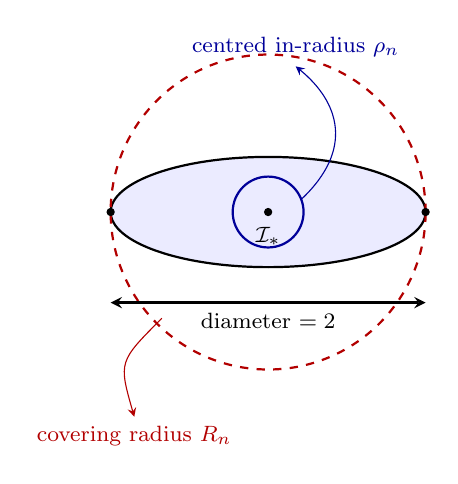
\begin{tikzpicture}[>=stealth]
  \fill[blue!8] (0,0) ellipse (2 and 0.7);
  \draw[thick] (0,0) ellipse (2 and 0.7);
  \draw[thick, blue!60!black] (0,0) circle (0.45);
  \draw[thick, red!70!black, dashed] (0,0) circle (2);
  \fill (0,0) circle (1.5pt) node[below=2pt, font=\footnotesize] {$\mathcal I_*$};
  \draw[->, blue!60!black] (0.42,0.16) .. controls (1.1,0.8) and (0.9,1.4) .. (0.35,1.85) node[anchor=south, font=\footnotesize, blue!60!black] {centred in-radius $\rho_n$};
  \draw[->, red!70!black] (-1.35,-1.35) .. controls (-1.9,-1.9) .. (-1.7,-2.6) node[anchor=north, font=\footnotesize, red!70!black] {covering radius $R_n$};
  \fill (-2,0) circle (1.5pt);
  \fill (2,0) circle (1.5pt);
  \draw[<->, thick] (-2,-1.15) -- (2,-1.15) node[midway, below, font=\footnotesize] {diameter $=2$};
\end{tikzpicture}
\hfil
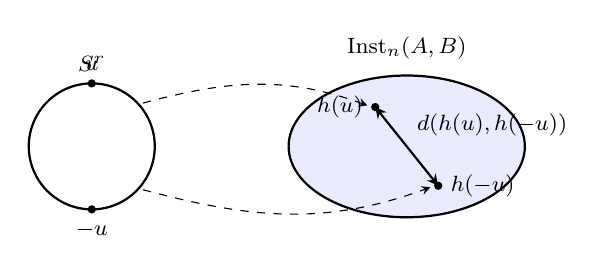
\begin{tikzpicture}[>=stealth]
  \draw[thick] (-2,0) circle (0.8);
  \node[font=\footnotesize] at (-2,1.05) {$S^r$};
  \fill (-2,0.8) circle (1.5pt) node[above=1pt, font=\footnotesize] {$u$};
  \fill (-2,-0.8) circle (1.5pt) node[below=1pt, font=\footnotesize] {$-u$};
  \fill[blue!8] (2,0) ellipse (1.5 and 0.9);
  \draw[thick] (2,0) ellipse (1.5 and 0.9);
  \node[font=\footnotesize] at (2,1.25) {$\Inst_n(A,B)$};
  \fill (1.6,0.5) circle (1.5pt) node[left=1pt, font=\footnotesize] {$h(u)$};
  \fill (2.4,-0.5) circle (1.5pt) node[right=1pt, font=\footnotesize] {$h(-u)$};
  \draw[<->, thick] (1.6,0.5) -- (2.4,-0.5) node[midway, above right, font=\footnotesize] {$d(h(u),h(-u))$};
  \draw[->, dashed] (-1.35,0.55) to[out=15, in=160] (1.5,0.52);
  \draw[->, dashed] (-1.35,-0.55) to[out=-15, in=200] (2.3,-0.52);
\end{tikzpicture}
\caption{The four radius notions of Remark~\ref{rem:radius-terminology}. Left: the centred in-radius $\rho_n$ (largest ball about $\mathcal I_*$ contained in the body), the covering radius $R_n$ (smallest ball about $\mathcal I_*$ containing the body), and the diameter, attained by two points of the body at distance $2$. Right: the antipodal profile: for a continuous map $h:S^r\to\Inst_n(A,B)$, $\alpha_r$ is, up to the factor $1/2$, the largest value of $\min_u d(h(u),h(-u))$ that can be forced; it is governed by antipodal separation, not by balls. The drawing is schematic; the numerical identity $\rho_n+R_n=2$ of Corollary~\ref{cor:complementarity} holds for the exact values of the instrument body, not for a generic convex set.}
\label{fig:radius-notions}
\end{figure}

\begin{proposition}[Monotonicity of profiles, widths, and envelopes]
\label{prop:monotonicity}
For every nonempty metric space $K$,
\[
\alpha_{r+1}(K)\le\alpha_r(K)\qquad(r\ge0),
\]
and if $K$ is compact then $0\le\alpha_r(K)\le\tfrac12\diam(K)$; consequently, if $\alpha_D(K)=0$ then $\alpha_r(K)=0$ for all $r\ge D$. For the instrument body,
\[
\delta_{r+1,\mathrm{inst}}^{\diamond}(A,B)\le\delta_{r,\mathrm{inst}}^{\diamond}(A,B),
\]
and the certified envelopes (Definitions~\ref{def:beta-best} and \ref{def:upper} below) satisfy
\[
\beta_{r+1}^{\mathrm{best},(n)}(A,B)\le\beta_r^{\mathrm{best},(n)}(A,B),\qquad
U_{r+1}^{(n)}(A,B)\le U_r^{(n)}(A,B).
\]
\end{proposition}

\begin{proof}
For the antipodal profile, let $h:S^{r+1}\to K$ be continuous and restrict it to an equatorial copy $S^r\simeq\{(x_0,\dots,x_{r+1})\in S^{r+1}:x_{r+1}=0\}$. The antipodal map on the equator is the ordinary antipodal map on $S^r$, hence
\[
\min_{u\in S^r}d(h(u),h(-u))
\ge\min_{u\in S^{r+1}}d(h(u),h(-u)).
\]
Taking one half and the supremum over all continuous $h:S^{r+1}\to K$ gives $\alpha_r(K)\ge\alpha_{r+1}(K)$. Distances are nonnegative, and $d(h(u),h(-u))\le\diam(K)$ for every $h$ and $u$, so $0\le\alpha_r(K)\le\tfrac12\diam(K)$. If $\alpha_D(K)=0$, the inequality $\alpha_r(K)\le\alpha_D(K)=0$ for $r\ge D$ follows by induction from $\alpha_{r+1}\le\alpha_r$, and $\alpha_r(K)\ge0$ always, so $\alpha_r(K)=0$ for all $r\ge D$.

For the widths, fix any continuous encoder $f:\Inst_n(A,B)\to\mathbb R^r$ and any decoder $g:\mathbb R^r\to\Inst_n(A,B)$, and define $f':\Inst_n(A,B)\to\mathbb R^{r+1}$ by $f'(x)=(f(x),0)$ and $g':\mathbb R^{r+1}\to\Inst_n(A,B)$ by $g'(z_1,\dots,z_{r+1})=g(z_1,\dots,z_r)$. Then $g'\circ f'=g\circ f$ pointwise, so the pair $(f',g')$ achieves the same error at latent dimension $r+1$ that $(f,g)$ achieves at dimension $r$; taking the infimum over $(f,g)$ gives $\delta_{r+1,\mathrm{inst}}^{\diamond}(A,B)\le\delta_{r,\mathrm{inst}}^{\diamond}(A,B)$.

For the lower envelope, the piecewise definition gives $\beta_0^{\mathrm{best},(n)}=R_n$, $\beta_r^{\mathrm{best},(n)}=1$ on $1\le r\le L_{A,B}^{(n)}$, $\gamma_{A,B}^{(n)}$ on $L_{A,B}^{(n)}<r<D_{A,B}^{(n)}$, and $0$ for $r\ge D_{A,B}^{(n)}$; since $nd_Bs\ge2$ gives $R_n\ge1$ and $0<\gamma_{A,B}^{(n)}\le1$ (Definition~\ref{def:beta-best}), the sequence is non-increasing.

For the upper envelope, each of the four families of admissible terms in Definition~\ref{def:upper} is monotone in $r$: the constant-code term is independent of $r$; the convex-projection term $2(D_{A,B}^{(n)}-r)/(D_{A,B}^{(n)}-r+1)$ is decreasing in $r$; and the pinching families are defined by threshold conditions $r\ge r_{\mathrm{out}}^{(n)}$ and $r\ge r_{\mathrm{in}}^{(n)}$, so every pinching term admissible at $r$ remains admissible at $r+1$, while further terms may become admissible. Hence every term entering $U_r^{(n)}$ is bounded below by a term entering $U_{r+1}^{(n)}$ (namely the same term, or a smaller newly available one), and $U_{r+1}^{(n)}(A,B)\le U_r^{(n)}(A,B)$.
\end{proof}

Let
\[
\Sstate_{\mathrm{flag}}(B\otimes C_n)
=\Big\{\tau=\sum_{k=1}^n\tau_k\otimes|k\rangle\langle k|:
\tau_k\ge0,\ \sum_{k=1}^n\Tr\tau_k=1\Big\}.
\]
For $\tau\in\Sstate_{\mathrm{flag}}(B\otimes C_n)$ define the replacement instrument $\vec{\mathcal R}_\tau$ by $(\vec{\mathcal R}_\tau)_k(X)=\Tr(X)\tau_k$; each component is completely positive and trace-nonincreasing and the sum is a channel. Write
\[
\RepInst_n(A,B)=\{\vec{\mathcal R}_\tau:\tau\in\Sstate_{\mathrm{flag}}(B\otimes C_n)\}.
\]

\begin{lemma}[Replacement-instrument isometry]
\label{lem:replacement-isometry}
For all flagged states $\tau,\sigma$,
\[
\|\vec{\mathcal R}_\tau-\vec{\mathcal R}_\sigma\|_{\diamond,\mathrm{inst}}
=\|\tau-\sigma\|_1=\sum_{k=1}^n\|\tau_k-\sigma_k\|_1.
\]
\end{lemma}

\begin{proof}
The flagged channel of $\vec{\mathcal R}_\tau$ is the replacement channel $X\mapsto\Tr(X)\tau$. For every reference-assisted input state $\xi$,
\[
(\id\otimes(\widehat{\vec{\mathcal R}_\tau}-\widehat{\vec{\mathcal R}_\sigma}))(\xi)
=\Tr_A(\xi)\otimes(\tau-\sigma),
\]
and $\Tr_A(\xi)$ is a state, so the trace norm equals $\|\tau-\sigma\|_1$ by multiplicativity; the supremum over inputs is unnecessary. The second equality follows from block diagonality in the flag.
\end{proof}

\begin{theorem}[Perfectly separated replacement instruments]
\label{thm:replacement-profile}
Assume $nd_B>1$. Replacement instruments contain a continuous image of $S^{nd_B^2-2}$ whose antipodes have instrument-diamond distance two, and consequently
\[
\alpha_r(\Inst_n(A,B))=1\qquad(0\le r\le nd_B^2-2).
\]
For the replacement family itself the profile is exact:
\[
\alpha_r(\RepInst_n(A,B))=
\begin{cases}
1,&0\le r\le nd_B^2-2,\\
0,&r\ge nd_B^2-1.
\end{cases}
\]
\end{theorem}

\begin{proof}
The real vector space of flag-block-diagonal Hermitian operators on $B\otimes C_n$ has dimension $nd_B^2$; its trace-zero subspace
\[
\mathfrak H_{\mathrm{flag},0}
=\Big\{X=\sum_{k=1}^nX_k\otimes|k\rangle\langle k|:
X_k\in\Herm(B),\ \sum_k\Tr X_k=0\Big\}
\]
has dimension $m:=nd_B^2-1$. Choose any Euclidean norm and let $S(\mathfrak H_{\mathrm{flag},0})\cong S^{m-1}=S^{nd_B^2-2}$ be its unit sphere. For $X$ on the sphere write the Jordan decomposition $X=X_+-X_-$; functional calculus preserves block diagonality and makes $X\mapsto X_+$ continuous. Since $X$ is nonzero and traceless, $t_X:=\Tr X_+=\Tr X_->0$. The map $h(X)=X_+/t_X$ is a continuous map into $\Sstate_{\mathrm{flag}}(B\otimes C_n)$ --- a continuous image of the sphere, and injectivity, which this map may lack, is not required by the antipodal-width arguments --- and $h(-X)=X_-/t_X$ has orthogonal support, so $\|h(X)-h(-X)\|_1=2$. Composing with the replacement embedding of Lemma~\ref{lem:replacement-isometry} gives the claimed sphere of instruments; equatorial restriction supplies every smaller index, and the reverse inequality follows from the diameter bound (Proposition~\ref{prop:diameter}).

For the replacement family above this range, Lemma~\ref{lem:replacement-isometry} identifies $\RepInst_n(A,B)$ affinely and isometrically with the compact convex body of flagged states inside a real affine space of dimension $m=nd_B^2-1$; choose an affine isomorphism of its affine hull with $\mathbb R^{m}$ and compose any continuous $h:S^r\to\RepInst_n(A,B)$ with it. For $r=m$, Borsuk--Ulam~\cite{Matousek2003} applied to $S^{m}\to\mathbb R^{m}$ produces an antipodal collision; for $r>m$, restrict the map to an equatorial $S^m\subset S^r$ first. Every such map therefore has minimum antipodal distance zero, proving the second part of the formula.
\end{proof}

\begin{remark}[In-radius versus antipodal profile]
\label{rem:inradius-vs-alpha}
$\rho_n=2/(nd_Bs)$ certifies a centrally symmetric norm ball in the full direction space $\mathfrak V_{A,B}^{(n)}$, while the sphere $S^{nd_B^2-2}$ via $X\mapsto X_+/\Tr X_+$ certifies a non-linear, antipodally $2$-separated sphere in the replacement body. There is no contradiction between $\rho_n<1$ and $\alpha_r=1$ for $r\le nd_B^2-2$: these are different geometric mechanisms (a ball radius versus an antipodal profile) acting on different subsets of the body. The ball bound governs the intermediate regime, while the replacement sphere governs the small-index regime.
\end{remark}

\begin{theorem}[Full-direction antipodal sphere]
\label{thm:full-direction}
Assume $nd_B>1$, and let $D=D_{A,B}^{(n)}$. For every $0\le r\le D-1$ there exists a continuous map $h:S^r\to\Inst_n(A,B)$ such that
\[
\|h(u)-h(-u)\|_{\diamond,\mathrm{inst}}\ge\frac2{d_A}
\qquad\forall u\in S^r.
\]
Consequently $\alpha_r(\Inst_n(A,B))\ge1/d_A$ for all $0\le r<D$. When $d_A=1$ the separation is $2$, hence $\alpha_r=1$ for all $r<D_{1,B}^{(n)}$, consistent with the exact replacement profile. For $n=1$ the construction restricts to the full-direction sphere of Ref.~\cite{CompanionChannels}.
\end{theorem}

\begin{proof}
Identify instruments with their normalised flagged Choi operators
\[
J\in\Herm(A_0\otimes B\otimes C_n),\qquad J\ge0,\qquad
\Tr_{B\otimes C_n}J=\frac{I_{A_0}}{d_A},
\]
flag-block-diagonal in $C_n$. The direction space
\[
\mathcal V=\big\{Z\in\Herm(A_0\otimes B\otimes C_n)_{\mathrm{flag}}:\Tr_{B\otimes C_n}Z=0\big\}
\]
has real dimension $D$. Equip $\mathcal V$ with a Euclidean norm and let $S(\mathcal V)\cong S^{D-1}$ be its unit sphere; it suffices to construct the map on $S^{D-1}$, since equatorial restriction supplies every smaller $r$. Fix the uniform flagged state
\[
\tau_0=\frac{I_B}{d_B}\otimes\frac{I_{C_n}}n.
\]
For $Z\in S(\mathcal V)$ write the Jordan decomposition $Z=Z_+-Z_-$ with $Z_+,Z_-\ge0$, $Z_+Z_-=0$; functional calculus preserves flag-block-diagonality. Since $\Tr_{B\otimes C_n}Z=0$,
\[
\Tr_{B\otimes C_n}Z_+=\Tr_{B\otimes C_n}Z_-.
\]
Let $t=\Tr Z_+=\Tr Z_-$. We claim $t>0$: if $t=0$ then $Z_+=0$, so $Z=-Z_-\le0$; but then $\Tr Z=\Tr_{A_0}\Tr_{B\otimes C_n}Z=0$ with $Z\le0$ forces $Z=0$, contradicting $Z\in S(\mathcal V)$. Define the normalised states
\[
\Theta_+=\frac{Z_+}{t},\qquad \Theta_-=\frac{Z_-}{t},
\]
which have orthogonal supports and share the same $A_0$-marginal
\[
\mu:=\Tr_{B\otimes C_n}\Theta_+=\Tr_{B\otimes C_n}\Theta_-.
\]
If $d_A=1$ the marginal condition is automatic ($A_0$ is one-dimensional and $\mu=1$), and we set $J^+(Z)=\Theta_+$, $J^-(Z)=\Theta_-$. Otherwise put $\lambda=1/d_A$. Since $\mu$ is a state on $A_0$, $\mu\le I_{A_0}$, hence $\lambda\mu\le I_{A_0}/d_A$. Define the correction state
\[
\nu=\frac{\frac{I_{A_0}}{d_A}-\lambda\mu}{1-\lambda}
=\frac{I_{A_0}-\mu}{d_A-1}\ge0,
\qquad \Tr\nu=1,
\]
and set
\[
J^+(Z)=\lambda\Theta_++(1-\lambda)\nu\otimes\tau_0,\qquad
J^-(Z)=\lambda\Theta_-+(1-\lambda)\nu\otimes\tau_0.
\]
Both $J^\pm(Z)$ are positive and flag-block-diagonal: the $\Theta_\pm$ summands inherit this property from $Z$ through the Jordan decomposition, and the correction term $\nu\otimes\tau_0$ is flag-block-diagonal because $\tau_0$ is diagonal in the fixed flag basis. Their common $A_0$-marginal is
\[
\lambda\mu+(1-\lambda)\nu=\frac{I_{A_0}}{d_A},
\]
so each is the normalised flagged Choi operator of an instrument; let $h(Z)$ be the instrument with Choi operator $J^+(Z)$. For $-Z$ the positive and negative parts are interchanged while $t$ and $\mu$ are unchanged, so $\nu$ is unchanged and $h(-Z)$ is the instrument with Choi operator $J^-(Z)$. The Choi difference is
\[
J^+(Z)-J^-(Z)=\lambda(\Theta_+-\Theta_-)
\]
(with $\lambda=1$ when $d_A=1$), and since $\Theta_+,\Theta_-$ are states with orthogonal supports,
\[
\|J^+(Z)-J^-(Z)\|_1=2\lambda=\frac2{d_A}.
\]
For any Hermiticity-preserving tuple $\vD$,
\[
\|\vD\|_{\diamond,\mathrm{inst}}\ge\|\Jhat_{\widehat{\vD}}\|_1,
\]
because testing the flagged map on the maximally entangled input state produces its normalised Choi operator. Therefore
\[
\|h(Z)-h(-Z)\|_{\diamond,\mathrm{inst}}\ge\frac2{d_A}.
\]
Finally, $Z\mapsto Z_+$ is continuous on Hermitian operators and $t=\Tr Z_+$ is continuous and strictly positive on the compact unit sphere $S(\mathcal V)$, hence bounded away from zero there; so $Z\mapsto J^+(Z)$ is continuous. Equatorial restriction proves the theorem for all $0\le r\le D-1$.
\end{proof}

\begin{remark}[Tunable mixing parameter]
\label{rem:tunable-lambda}
In the proof of Theorem~\ref{thm:full-direction}, the mixing parameter may be chosen as a function of $Z$: since $\mu=\mu(Z)$ is a state on $A_0$ we have $\|\mu\|_\infty\in[1/d_A,1]$, and $I_{A_0}/d_A-\lambda\mu\ge0$ holds if and only if $\lambda\le1/(d_A\|\mu\|_\infty)$. Taking $\lambda(Z)=1/(d_A\|\mu(Z)\|_\infty)\in[1/d_A,1]$ therefore increases the pointwise separation to
\[
\|J^+(Z)-J^-(Z)\|_1=\frac{2}{d_A\|\mu(Z)\|_\infty}\ge\frac2{d_A},
\]
with $\lambda=1$ exactly when $\mu(Z)=I_{A_0}/d_A$, in which case no correction state is needed. The uniform certificate $\alpha_r\ge1/d_A$ is unchanged. The proof of Theorem~\ref{thm:full-direction} uses the constant value $\lambda=1/d_A$, which makes continuity of the construction immediate. Near points with $\mu(Z)=I_{A_0}/d_A$ the correction state $\nu(Z)=(I_{A_0}/d_A-\lambda(Z)\mu(Z))/(1-\lambda(Z))$ becomes an indeterminate quotient: the weight $1-\lambda(Z)$ tends to zero while the vanishing of the numerator depends on the approach direction, so a variable $\lambda$ would require a separate gluing argument at exactly those points.
\end{remark}

\begin{corollary}[Antipodal cutoff at affine dimension]
\label{cor:cutoff}
Assume $nd_B>1$. Then $\alpha_r(\Inst_n(A,B))=0$ for all $r\ge D_{A,B}^{(n)}$.
\end{corollary}

\begin{proof}
Choose affine coordinates $c:\mathfrak A_{A,B}^{(n)}\to\mathbb R^{D}$ (an affine isomorphism, hence injective). For any continuous $h:S^r\to\Inst_n(A,B)$ with $r\ge D$, restrict to an equatorial $S^D\subset S^r$; Borsuk--Ulam applied to $c\circ h:S^D\to\mathbb R^D$ gives $u$ with $c(h(u))=c(h(-u))$, hence $h(u)=h(-u)$ by injectivity. Thus $\alpha_D=0$, and monotonicity (Proposition~\ref{prop:monotonicity}) extends this to all $r\ge D$.
\end{proof}

\begin{theorem}[Observable antipodal sphere]
\label{thm:observable}
Assume either (i) $n\ge2$ and $d_A\ge2$, or (ii) $n=1$, $d_A\ge2$, $d_B\ge2$. Then there exists a continuous map $h:S^{d_A^2-2}\to\Inst_n(A,B)$ whose antipodal images have instrument-diamond distance $2$; consequently
\[
\alpha_r(\Inst_n(A,B))=1\qquad(0\le r\le d_A^2-2).
\]
For $n=1$ this is the observable sphere of Ref.~\cite{CompanionChannels}. The construction is a continuous image of the sphere and may fail to be injective: $H$ and its positive scalar multiples define the same instrument. Injectivity is not required by the width arguments.
\end{theorem}

\begin{proof}
First suppose $n\ge2$. Fix a unit vector $|b_0\rangle\in B$ and let $\sigma=|b_0\rangle\langle b_0|$. For $H\in\Herm_0(A)$, $H\neq0$, define
\[
K(H)=\frac{H}{\|H\|_\infty},\qquad E_\pm(H)=\frac{I_A\pm K(H)}2.
\]
Then $E_\pm(H)\ge0$ and $E_+(H)+E_-(H)=I_A$. Define an instrument by
\[
\mathcal I^H_1(X)=\Tr(E_+(H)X)\sigma,\qquad
\mathcal I^H_2(X)=\Tr(E_-(H)X)\sigma,\qquad
\mathcal I^H_k(X)=0\ (k\ge3);
\]
the sum is the replacement channel $X\mapsto\Tr(X)\sigma$, so $\mathcal I^H\in\Inst_n(A,B)$. Since $\|K(H)\|_\infty=1$, $K(H)$ has a unit eigenvector $|\psi\rangle$ with eigenvalue $\varepsilon\in\{+1,-1\}$. Then
\[
\Tr(E_{\varepsilon}(H)|\psi\rangle\langle\psi|)=1,\qquad
\Tr(E_{-\varepsilon}(H)|\psi\rangle\langle\psi|)=0,
\]
where $E_{+1}(H)=E_+(H)$ and $E_{-1}(H)=E_-(H)$; since $E_\pm(-H)=E_\mp(H)$, the two effects are exchanged for $-H$. Hence the flagged outputs of $\mathcal I^H$ and $\mathcal I^{-H}$ on the input $|\psi\rangle\langle\psi|$ are $\sigma\otimes|1\rangle\langle1|$ and $\sigma\otimes|2\rangle\langle2|$ in one order or the other, which are orthogonal, so their trace norm difference is $2$; by the diameter bound the instrument distance is exactly $2$. The map $H\mapsto H/\|H\|_\infty$ is continuous on the Euclidean unit sphere of $\Herm_0(A)\cong\mathbb R^{d_A^2-1}$, so the construction gives a continuous image of $S^{d_A^2-2}$ with antipodal distance $2$; equatorial restriction gives the result for all $0\le r\le d_A^2-2$.

For $n=1$ and $d_B\ge2$, choose two orthogonal pure output states $\sigma_\pm=|\varphi_\pm\rangle\langle\varphi_\pm|$ and define the channel
\[
\Phi^H(X)=\Tr(E_+(H)X)\sigma_++\Tr(E_-(H)X)\sigma_-.
\]
The same eigenvector witness gives orthogonal outputs $\sigma_+$ and $\sigma_-$, hence distance $2$, and the continuity argument is identical.
\end{proof}

\begin{proposition}[Orthogonal join of flagged state spheres]
\label{prop:join}
Let $W_1,\dots,W_\ell$ be pairwise orthogonal flag-block-diagonal subspaces of $B\otimes C_n$, and suppose that continuous maps $h_i:S^{r_i}\to\Sstate_{\mathrm{flag}}(B\otimes C_n)$ take values in states supported on $W_i$ and satisfy
\[
\|h_i(u)-h_i(-u)\|_1=2\qquad(u\in S^{r_i}).
\]
Then there is a continuous map $H:S^{\sum_i r_i+\ell-1}\to\Sstate_{\mathrm{flag}}(B\otimes C_n)$ with
\[
\|H(y)-H(-y)\|_1=2
\]
for every $y$. Composing with the replacement-instrument embedding gives the same antipodal separation in instrument diamond norm.
\end{proposition}

\begin{proof}
View the domain sphere as the unit sphere of $\bigoplus_{i=1}^{\ell}\mathbb R^{r_i+1}$. For a point $y=(y_1,\dots,y_\ell)$ on it, write
$\lambda_i=\|y_i\|_2^2$ and, on the blocks with $y_i\neq0$, $u_i=y_i/\|y_i\|_2$; then define
\[
H(y)=\sum_{i:y_i\neq0}\lambda_i\,h_i(u_i),
\]
reading the $i$-th summand as zero when $y_i=0$. The weights satisfy $\sum_i\lambda_i=1$, so $H(y)$ is a flagged state. Continuity at points where some $y_i=0$ follows because the trace norm of the $i$-th summand is $\|\lambda_i h_i(u_i)\|_1=\lambda_i\to0$ as $y_i\to0$, uniformly in the direction $u_i$. Because the supports $W_i$ are pairwise orthogonal, the difference $H(y)-H(-y)$ is block diagonal with respect to $\bigoplus_iW_i$, so
\[
\|H(y)-H(-y)\|_1
=\sum_i\lambda_i\|h_i(u_i)-h_i(-u_i)\|_1
=2\sum_i\lambda_i=2.
\]
Lemma~\ref{lem:replacement-isometry} transfers the equality to replacement instruments.
\end{proof}

\begin{proposition}[Instrument-level join with replacement spheres]
\label{prop:join-inst}
Let $W\subseteq B\otimes C_n$ be a flag-block-diagonal subspace. Let $h:S^{r_1}\to\Inst_n(A,B)$ be continuous and such that
\begin{enumerate}[leftmargin=*,itemsep=2pt]
\item for every input state $\rho$ on $A_0\otimes A$ and every $u\in S^{r_1}$, the flagged output $(\id_{A_0}\otimes\widehat{h(u)})(\rho)$ is supported on $A_0\otimes W$, and
\item $\|h(u)-h(-u)\|_{\diamond,\mathrm{inst}}=2$ for every $u\in S^{r_1}$.
\end{enumerate}
Let $\tau:S^{r_2}\to\Sstate_{\mathrm{flag}}(B\otimes C_n)$ be continuous, take values in states supported on the per-block orthogonal complement $W^{\perp}$, and satisfy $\|\tau(v)-\tau(-v)\|_1=2$ for every $v\in S^{r_2}$. Then, on the unit sphere of $\mathbb R^{r_1+1}\oplus\mathbb R^{r_2+1}$,
\[
\mathcal I(y)=\|y_1\|_2^2\,h\!\left(\frac{y_1}{\|y_1\|_2}\right)
+\|y_2\|_2^2\,\vec{\mathcal R}_{\tau(y_2/\|y_2\|_2)}
\]
(with a summand read as zero when the corresponding coordinate block vanishes) defines a continuous map $S^{r_1+r_2+1}\to\Inst_n(A,B)$ with
\[
\|\mathcal I(y)-\mathcal I(-y)\|_{\diamond,\mathrm{inst}}=2\qquad(y\in S^{r_1+r_2+1}).
\]
\end{proposition}

\begin{proof}
Both summands are convex combinations of instruments, hence instruments, so $\mathcal I(y)\in\Inst_n(A,B)$; the instrument body is bounded (every flagged channel has diamond norm $1$), so each summand tends to zero in norm as its weight tends to zero, uniformly over the sphere, which gives continuity on the coordinate spheres $\{y_i=0\}$ exactly as in Proposition~\ref{prop:join}. Fix $y$ and write $\lambda=\|y_1\|_2^2$. The endpoint cases reduce to single components: at $\lambda=0$ the pair is the replacement pair, at distance $2$ by Lemma~\ref{lem:replacement-isometry}, and at $\lambda=1$ it is the observable pair, at distance $2$ by hypothesis (ii). Assume $0<\lambda<1$, write $u=y_1/\|y_1\|_2$ and $v=y_2/\|y_2\|_2$, and set $\vD_1=h(u)-h(-u)$ and $\vD_2=\vec{\mathcal R}_{\tau(v)}-\vec{\mathcal R}_{\tau(-v)}$, so that $\mathcal I(y)-\mathcal I(-y)=\lambda\vD_1+(1-\lambda)\vD_2$. The set of input states is compact and $\rho\mapsto\|(\id\otimes\vD_1)(\rho)\|_1$ is continuous with supremum $\|\vD_1\|_{\diamond,\mathrm{inst}}=2$, so there is an input state $\rho_*$ with $\|(\id\otimes\vD_1)(\rho_*)\|_1=2$. For this same input, Lemma~\ref{lem:replacement-isometry} gives $(\id\otimes\vD_2)(\rho_*)=\Tr_A(\rho_*)\otimes(\tau(v)-\tau(-v))$, of trace norm $\|\tau(v)-\tau(-v)\|_1=2$, independently of $\rho_*$. By (i) applied to $h(u)$ and $h(-u)$, the Hermitian operator $(\id\otimes\vD_1)(\rho_*)$ is supported on $A_0\otimes W$, while $(\id\otimes\vD_2)(\rho_*)$ is supported on $A_0\otimes W^{\perp}$; orthogonal supports make the trace norm additive, so
\[
\big\|(\id\otimes(\mathcal I(y)-\mathcal I(-y)))(\rho_*)\big\|_1
=\lambda\cdot2+(1-\lambda)\cdot2=2.
\]
Hence $\|\mathcal I(y)-\mathcal I(-y)\|_{\diamond,\mathrm{inst}}\ge2$, and the reverse inequality is the diameter bound (Proposition~\ref{prop:diameter}).
\end{proof}

\begin{remark}[Why the join carries at most one input-dependent sphere]
\label{rem:join-one-observable}
Proposition~\ref{prop:join-inst} joins one \emph{input-dependent} sphere with replacement spheres: the replacement components attain their maximal separation $2$ on \emph{every} input, so an input that exposes the input-dependent component simultaneously exposes all of them. Two input-dependent components could not be joined by this mechanism, since their separating inputs (eigenvectors of the respective observables) vary with the sphere parameter and need not coincide; this is why exactly one observable sphere enters Corollary~\ref{cor:join-dimension} below.
\end{remark}

\begin{corollary}[Observable--replacement join dimension]
\label{cor:join-dimension}
Under the hypotheses of Theorem~\ref{thm:observable}, the flagged outputs of the observable sphere are supported on the flagged subspace
\[
W_{\mathrm{obs}}=\operatorname{span}\{|b_0\rangle\otimes|1\rangle,\ |b_0\rangle\otimes|2\rangle\}
\]
in the case $n\ge2$ (with the pure state $\sigma=|b_0\rangle\langle b_0|$), and on the two-dimensional flagged subspace $W_{\mathrm{obs}}=\operatorname{span}\{|\varphi_+\rangle,|\varphi_-\rangle\}$ in the case $n=1$, where $\sigma_\pm=|\varphi_\pm\rangle\langle\varphi_\pm|$ are the two orthogonal output states of the channel construction. Let $W_{\mathrm{obs}}^{\perp}$ denote the per-block orthogonal complement of $W_{\mathrm{obs}}$: when $n\ge2$ its first two blocks are $\{|b_0\rangle\}^{\perp}\subseteq B$ and its remaining $n-2$ blocks are all of $B$; when $n=1$ it is the orthogonal complement of $W_{\mathrm{obs}}$ in $B$. The real vector space of flag-block-diagonal Hermitian operators supported on $W_{\mathrm{obs}}^{\perp}$ has dimension
\[
N_{\mathrm{join}}=
\begin{cases}
2(d_B-1)^2+(n-2)d_B^2,&n\ge2,\\
(d_B-2)^2,&n=1.
\end{cases}
\]
If $N_{\mathrm{join}}\ge1$, then
\[
\alpha_r(\Inst_n(A,B))=1\qquad(0\le r\le d_A^2+N_{\mathrm{join}}-3).
\]
The boundary value $N_{\mathrm{join}}=1$, which occurs only for $n=1$, $d_B=3$, is degenerate: the replacement sphere $S^{N_{\mathrm{join}}-2}=S^{-1}$ is empty, the join reduces to the observable sphere alone, and the displayed formula reproduces its index $d_A^2-2$.
For $n=1$ this is the observable--replacement join of Ref.~\cite{CompanionChannels}.
\end{corollary}

\begin{proof}
The observable sphere $h:S^{d_A^2-2}\to\Inst_n(A,B)$ of Theorem~\ref{thm:observable} is continuous and has antipodal instrument-diamond distance $2$; on every input $\rho$, each outcome component of its flagged output is a positive operator on $A_0$ tensored with $\sigma\otimes|k\rangle\langle k|$, $k\in\{1,2\}$ (respectively with $\sigma_+$ or $\sigma_-$ when $n=1$), and the remaining outcomes vanish, so all flagged outputs are supported on $A_0\otimes W_{\mathrm{obs}}$, i.e.\ hypothesis (i) of Proposition~\ref{prop:join-inst} holds with $W=W_{\mathrm{obs}}$. The per-block complement $W_{\mathrm{obs}}^{\perp}$ is itself flag-block-diagonal, and the Jordan construction of Theorem~\ref{thm:replacement-profile}, applied to the traceless part of the real vector space of flag-block-diagonal Hermitian operators supported on $W_{\mathrm{obs}}^{\perp}$, produces a continuous sphere $\tau:S^{N_{\mathrm{join}}-2}\to\Sstate_{\mathrm{flag}}(B\otimes C_n)$ of states supported on $W_{\mathrm{obs}}^{\perp}$ with $\|\tau(v)-\tau(-v)\|_1=2$; the condition $N_{\mathrm{join}}\ge2$ guarantees nonemptiness of this sphere, while at $N_{\mathrm{join}}=1$ the traceless block space is trivial, the sphere is empty, and the observable sphere alone realises the displayed range, so the statement holds for $N_{\mathrm{join}}\ge1$. Proposition~\ref{prop:join-inst} joins the two spheres into a continuous map
\[
S^{(d_A^2-2)+(N_{\mathrm{join}}-2)+1}=S^{d_A^2+N_{\mathrm{join}}-3}\longrightarrow\Inst_n(A,B)
\]
with antipodal instrument-diamond distance $2$; equatorial restriction supplies every smaller index, and $\alpha_r\le1$ always by the diameter bound (Proposition~\ref{prop:diameter}).
\end{proof}

\begin{remark}[Structured partitions]
\label{rem:partitions}
The $\ell$-fold join of Proposition~\ref{prop:join} may also be applied to arbitrary pairwise orthogonal output--flag blocks $(B_i,n_i)$ with $\sum_ib_i\le d_B$, $\sum_in_i=n$, producing a sphere of dimension $\sum_i(n_ib_i^2-1)-1$ whenever $n_ib_i^2\ge2$ for every retained block. Taking one block with $b_1=d_B$, $n_1=n$ recovers the leading dimension $nd_B^2-2$; no partition improves Theorem~\ref{thm:replacement-profile}.
\end{remark}

\begin{definition}[Certified one-sphere dimension]
\label{def:one-sphere}
Let
\[
L_{\mathrm{rep}}=nd_B^2-2,
\]
valid whenever $nd_B>1$. If either $n\ge2,d_A\ge2$, or $n=1,d_A\ge2,d_B\ge2$, set $L_{\mathrm{obs}}=d_A^2-2$; otherwise set $L_{\mathrm{obs}}=-1$. If the observable sphere is valid and $N_{\mathrm{join}}\ge1$ (Corollary~\ref{cor:join-dimension}), set $L_{\mathrm{join}}=d_A^2+N_{\mathrm{join}}-3$ (at the degenerate value $N_{\mathrm{join}}=1$, occurring only for $n=1$, $d_B=3$, this equals $L_{\mathrm{obs}}$); otherwise $L_{\mathrm{join}}=-1$. Finally define
\[
L_{A,B}^{(n)}
=\min\Big\{D_{A,B}^{(n)}-1,\ \max\{L_{\mathrm{rep}},L_{\mathrm{obs}},L_{\mathrm{join}}\}\Big\},
\]
where invalid terms ($-1$) are ignored. If $d_A=1$, the observable and join terms are invalid and $L_{1,B}^{(n)}=nd_B^2-2=D_{1,B}^{(n)}-1$.
\end{definition}

\begin{definition}[Certified lower envelope]
\label{def:beta-best}
Assume $nd_B>1$. Let
\[
\rho_n=\frac{2}{nd_B\min\{d_A,d_B\}},\qquad
\gamma_{A,B}^{(n)}=\max\Big\{\rho_n,\frac1{d_A}\Big\}.
\]
Define
\[
\beta_r^{\mathrm{best},(n)}(A,B)=
\begin{cases}
R_n=2\big(1-\tfrac{1}{nd_Bs}\big),&r=0,\\[3pt]
1,&1\le r\le L_{A,B}^{(n)},\\[3pt]
\gamma_{A,B}^{(n)},&L_{A,B}^{(n)}<r<D_{A,B}^{(n)},\\[6pt]
0,&r\ge D_{A,B}^{(n)}.
\end{cases}
\]
When $L_{A,B}^{(n)}=D_{A,B}^{(n)}-1$ the middle range is empty (this is always the case for $d_A=1$). The value at $r=0$ is the exact constant-code width of Corollary~\ref{cor:constant-code}: the envelope is upgraded there from the one-sphere value $1$ to $R_n$, so the lower and upper envelopes coincide at $r=0$. Since $nd_Bs\ge2$ gives $R_n\ge1$ and $d_A\ge1$ gives $0<\gamma_{A,B}^{(n)}\le1$, the displayed envelope is non-increasing in $r$. Every component is rigorously certified by Theorems~\ref{thm:replacement-profile}, \ref{thm:full-direction}, \ref{thm:observable}, Corollary~\ref{cor:join-dimension}, and Theorem~\ref{thm:ball}, and, at $r=0$, Corollary~\ref{cor:constant-code}.
\end{definition}

\begin{remark}[Resource interpretation of the two breakpoints]
\label{rem:breakpoints}
The two breakpoints of the envelope have a direct resource interpretation. A flagged output state has $nd_B^2-1$ affine parameters, while an input-dependent instrument has $d_A^2(nd_B^2-1)$. The first regime ($r\le L_{A,B}^{(n)}$) is already obstructed by preparing and recording one classical--quantum output state --- augmented by the observable constructions, which obstruct input-dependent effect readout even when the output state is fixed. The second regime concerns the additional dependence of all outcome branches on the input operator. Increasing the number of outcomes therefore has two opposite effects: it linearly enlarges the global representation space, while dividing the local positivity margin of the uniform instrument by $n$.
\end{remark}

\begin{remark}[Two mechanisms behind the intermediate floor]
\label{rem:gamma-mechanisms}
The intermediate floor $\gamma_{A,B}^{(n)}=\max\{\rho_n,1/d_A\}$ combines two certificates of different geometric origin, and the maximum is the correct combination because each term is individually a valid lower bound on every width in the intermediate regime. The term $\rho_n=2/(nd_Bs)$ is a local statement: a ball of radius $\rho_n$ about the uniform instrument exists, and the antipodal pairs inside a centrally symmetric ball certify error at least $\rho_n$ via the radial map (Corollary~\ref{cor:intrinsic}); it decays with $n$ because the uniform trace budget is split among $n$ outcomes. The term $1/d_A$ is a global statement: a sphere spanning all $D_{A,B}^{(n)}$ directions of the body exists whose antipodes are separated by $2/d_A$ (Theorem~\ref{thm:full-direction}); the value $1/d_A$ is the largest mixing weight at which two orthogonal flagged Choi states with a common input marginal can be completed to instruments uniformly over all directions, the direction-dependent optimum $1/(d_A\|\mu(Z)\|_\infty)$ of Remark~\ref{rem:tunable-lambda} attaining its worst-case value $1/d_A$ exactly when the common marginal is pure. The two terms trade off at $n\approx2d_A/(d_B\min\{d_A,d_B\})$: below this threshold the ball term dominates the maximum, above it the input-dimension term $1/d_A$ is the floor; in particular, whenever $d_A\le d_B$ the floor is $1/d_A$ for every $n\ge2$. This is the geometric reason the intermediate obstruction carries an $n$-independent component. The $n=1$ value $\gamma_{A,B}^{(1)}=\max\{2/(d_B\min\{d_A,d_B\}),1/d_A\}$ is the intermediate envelope value of Ref.~\cite{CompanionChannels}.
\end{remark}

\section{Compression widths: upper bounds and exact thresholds}
\label{sec:widths}

The spheres of the preceding section certify that certain widths are large; this section supplies the constructive upper bounds and the exact threshold where the width collapses to zero. The two sides bracket every intermediate width in an explicit interval. The widths defined below are continuous-encoding analogues of the classical Kolmogorov widths of a compact set in a normed space~\cite{Pinkus1985}, with the approximating linear subspaces of the classical theory replaced by arbitrary continuous encodings into $\mathbb R^r$.

\begin{convention}[Continuous encoding, unrestricted decoding]
\label{conv:decoder}
Throughout the compression-width results, an encoder is required to be continuous while the decoder is unrestricted unless explicitly stated otherwise. This convention is essential for the Helly-type upper bounds; where a continuous decoder is available we state this separately.
\end{convention}

\begin{definition}[Euclidean instrument width]
\label{def:width}
\[
\delta_{r,\mathrm{inst}}^{\diamond}(A,B)
=\inf_{\substack{f:\Inst_n(A,B)\to\mathbb R^r\ \text{continuous}\\ g:\mathbb R^r\to\Inst_n(A,B)}}
\sup_{\mathcal I\in\Inst_n(A,B)}
\|g(f(\mathcal I))-\mathcal I\|_{\diamond,\mathrm{inst}}.
\]
For compact metric $K\subseteq L$ we also use $\delta_r^{\mathrm c}(K;L)$, the analogous width with continuous encoders into $\mathbb R^r$ and arbitrary (not necessarily continuous) decoders into $L$.
\end{definition}

\begin{remark}[Decoder codomain does not weaken the lower bounds]
\label{rem:decoder-codomain}
Since $\RepInst_n(A,B)\subset\Inst_n(A,B)\subset\mathfrak A_{A,B}^{(n)}$, and the triangle inequality $\|h(u)-\Psi\|_{\diamond,\mathrm{inst}}+\|h(-u)-\Psi\|_{\diamond,\mathrm{inst}}\ge\|h(u)-h(-u)\|_{\diamond,\mathrm{inst}}$ holds for every $\Psi$ in the ambient vector space $\bigoplus_k\Lin(A,B)$, the lower bounds of Corollaries~\ref{cor:intrinsic} and \ref{cor:euclidean} (stated below) are proved for decoders with values in the full affine space $\mathfrak A_{A,B}^{(n)}$ --- a strictly stronger statement than for instrument-valued decoders. Hence
\begin{align*}
\beta_r^{\mathrm{best},(n)}(A,B)
&\le\delta_r^{\mathrm c}\big(\Inst_n(A,B);\mathfrak A_{A,B}^{(n)}\big)\\
&\le\delta_r^{\mathrm c}\big(\Inst_n(A,B);\Inst_n(A,B)\big)
=\delta_{r,\mathrm{inst}}^{\diamond}(A,B)
\le U_r^{(n)}(A,B).
\end{align*}
Allowing unphysical affine decoders cannot circumvent the certified lower envelope; and because the optimal constant-code centre $\mathcal I_*$ is itself an instrument (Theorem~\ref{thm:covering}), the constant-code width coincides over both codomains (Corollary~\ref{cor:constant-code}), so every upper bound of this paper is admissible with a physical instrument decoder. The same codomain convention underlies the Hermiticity-preserving trace-preserving decoder bounds of Ref.~\cite{CompanionChannels}.
\end{remark}

\begin{corollary}[Certified width bracket]
\label{cor:bracket}
Assume $nd_B>1$. For $0\le r<D_{A,B}^{(n)}$,
\[
\beta_r^{\mathrm{best},(n)}(A,B)
\le\delta_{r,\mathrm{inst}}^{\diamond}(A,B)
\le U_r^{(n)}(A,B),
\]
where $U_r^{(n)}$ is defined in Definition~\ref{def:upper}. For $r\ge D_{A,B}^{(n)}$ the width is zero.
\end{corollary}

\begin{proof}
At $r=0$ every encoder is constant, and Corollary~\ref{cor:constant-code} gives $\delta_{0,\mathrm{inst}}^{\diamond}(A,B)=R_n=\beta_0^{\mathrm{best},(n)}(A,B)=U_0^{(n)}(A,B)$, so the bracket is exact at $r=0$. For $1\le r\le L_{A,B}^{(n)}$ the replacement sphere, observable sphere, or observable--replacement join supplies a continuous map $h:S^r\to\Inst_n(A,B)$ with antipodal distance $2$; composing with any continuous encoder $f$ gives $f\circ h:S^r\to\mathbb R^r$, and Borsuk--Ulam produces $u$ with $f(h(u))=f(h(-u))$. The decoder returns one reconstruction for the pair, and the triangle inequality forces error at least $1=\beta_r^{\mathrm{best},(n)}$. The argument applies verbatim to decoders valued in the ambient affine space $\mathfrak A_{A,B}^{(n)}$ (Remark~\ref{rem:decoder-codomain}), which only strengthens the lower bound. For $L_{A,B}^{(n)}<r<D_{A,B}^{(n)}$, two independent certificates hold: the centred ball gives antipodal separation $2\rho_n$ (via the radial map of Corollary~\ref{cor:intrinsic}, which needs only $r+1\le D_n$), and Theorem~\ref{thm:full-direction} gives separation $2/d_A$. Choose the radial map if $\rho_n\ge1/d_A$ and the full-direction map if $1/d_A\ge\rho_n$; the chosen map has separation $2\gamma_{A,B}^{(n)}$, hence error at least $\gamma_{A,B}^{(n)}$. The upper terms are Theorem~\ref{thm:covering}, Theorem~\ref{thm:pinching} and Proposition~\ref{prop:convex} (stated below); exact reconstruction for $r\ge D_{A,B}^{(n)}$ is Theorem~\ref{thm:zero-error}.
\end{proof}

For a Hausdorff latent space $Y$, recall the deleted product
\[
F_2(Y)=\{(y_0,y_1)\in Y^2:y_0\neq y_1\}
\]
with the involution exchanging the two entries, and let
\[
\coind F_2(Y)
=\sup\big\{k\ge0:\exists\ \text{equivariant}\ S^k\to F_2(Y)\big\},
\]
with value $-1$ when $F_2(Y)$ is empty and possible value $+\infty$. For a metric space $Y$, $F_2(Y)$ carries the subspace topology of $Y^2$ and the free $\mathbb Z_2$-action; Hausdorffness is not needed for the deleted product itself, but is natural to make the diagonal closed. If $\coind F_2(Y)=+\infty$, no integer $q$ satisfies $q>\coind F_2(Y)$ and the corollary below is vacuous. For $r\ge1$, if $Y$ admits a continuous injection $\jmath:Y\to\mathbb R^r$, the normalised difference map
\[
(y_0,y_1)\longmapsto\frac{\jmath(y_0)-\jmath(y_1)}{\|\jmath(y_0)-\jmath(y_1)\|_2}
\]
is continuous and equivariant $F_2(Y)\to S^{r-1}$, so by Borsuk--Ulam~\cite{Matousek2003}, $\coind F_2(Y)\le r-1$.

\begin{corollary}[Intrinsic latent-space instrument hierarchy]
\label{cor:intrinsic}
Assume $nd_B>1$. Let $Y$ be Hausdorff and let $q\in\mathbb N_0$ satisfy
\[
q>\coind F_2(Y).
\]
Then every continuous encoder $\operatorname{Enc}:\Inst_n(A,B)\to Y$ and every decoder $\operatorname{Dec}:Y\to\mathfrak A_{A,B}^{(n)}$ satisfy
\[
\sup_{\mathcal I\in\Inst_n(A,B)}
\|\operatorname{Dec}(\operatorname{Enc}(\mathcal I))-\mathcal I\|_{\diamond,\mathrm{inst}}
\ge\beta_q^{\mathrm{best},(n)}(A,B).
\]
\end{corollary}

\begin{proof}
If $q\ge D_{A,B}^{(n)}$, then $\beta_q^{\mathrm{best},(n)}(A,B)=0$ and the claimed inequality is trivial; assume henceforth $q<D_{A,B}^{(n)}$. If $q=0$, the hypothesis $q>\coind F_2(Y)$ forces $F_2(Y)=\varnothing$, i.e.\ $Y$ is a singleton; the decoder returns a single point $\Psi\in\mathfrak A_{A,B}^{(n)}$, and the centre-optimality clause of Theorem~\ref{thm:covering} gives $\sup_{\mathcal I}\|\Psi-\mathcal I\|_{\diamond,\mathrm{inst}}=R_{\mathrm{inst}}(\Psi)\ge R_n=\beta_0^{\mathrm{best},(n)}(A,B)$. If $1\le q\le L_{A,B}^{(n)}$, restrict the perfectly separated sphere supplied by Theorem~\ref{thm:replacement-profile}, Theorem~\ref{thm:observable}, or Corollary~\ref{cor:join-dimension} to an equatorial $S^q$. If $L_{A,B}^{(n)}<q<D_{A,B}^{(n)}$, then $q+1\le D_{A,B}^{(n)}$; choose a $(q+1)$-dimensional subspace $W\subseteq\mathfrak V_{A,B}^{(n)}$ and use the radial map
\[
h(u)=\mathcal I_*+\rho_n\frac{u}{\|u\|_{\diamond,\mathrm{inst}}}
\]
on an auxiliary Euclidean sphere $S^q\subset W$ (the denominator $\|u\|_{\diamond,\mathrm{inst}}$ is a continuous and strictly positive function on the compact Euclidean sphere, so the normalisation is continuous). Theorem~\ref{thm:ball} makes the radial map instrument-valued with antipodal separation $2\rho_n$, and Theorem~\ref{thm:full-direction} independently supplies a map with separation $2/d_A$; choose the radial map when $\rho_n\ge1/d_A$ and the full-direction map otherwise, so that the chosen map has antipodal separation $2\gamma_{A,B}^{(n)}$. In both regimes, if the two latent codes $\operatorname{Enc}(h(u))$ and $\operatorname{Enc}(h(-u))$ were distinct for every $u$, then $u\mapsto(\operatorname{Enc}(h(u)),\operatorname{Enc}(h(-u)))$ would be an equivariant map $S^q\to F_2(Y)$, contradicting the coindex hypothesis. An antipodal pair therefore has one code; the decoder returns one reconstruction for it, and the triangle inequality gives half the separation, namely $\beta_q^{\mathrm{best},(n)}(A,B)$.
\end{proof}

\begin{corollary}[Continuous instrument-compression hierarchy]
\label{cor:euclidean}
Assume $nd_B>1$, and let $Y$ admit a continuous injection into $\mathbb R^r$. Then, for every continuous encoder $\operatorname{Enc}:\Inst_n(A,B)\to Y$ and every decoder $\operatorname{Dec}:Y\to\mathfrak A_{A,B}^{(n)}$,
\[
\sup_{\mathcal I\in\Inst_n(A,B)}
\|\operatorname{Dec}(\operatorname{Enc}(\mathcal I))-\mathcal I\|_{\diamond,\mathrm{inst}}
\ge\beta_r^{\mathrm{best},(n)}(A,B).
\]
\end{corollary}

\begin{proof}
If $r=0$ then $Y$ has at most one point and $F_2(Y)=\emptyset$ has coindex $-1$; if $r\ge1$ the normalised difference map gives $\coind F_2(Y)\le r-1$ as above. Apply Corollary~\ref{cor:intrinsic} with $q=r$.
\end{proof}

\begin{theorem}[Zero-error threshold, with continuous decoding at the threshold]
\label{thm:zero-error}
For Euclidean latent spaces and under Convention~\ref{conv:decoder},
\[
\delta_{r,\mathrm{inst}}^{\diamond}(A,B)=0
\quad\Longleftrightarrow\quad
r\ge D_{A,B}^{(n)}.
\]
Moreover, for every $r\ge D_{A,B}^{(n)}$, exact decoding may be chosen continuous.
\end{theorem}

\begin{proof}
For $r\ge D_{A,B}^{(n)}$, choose affine coordinates $c:\mathfrak A_{A,B}^{(n)}\to\mathbb R^{D}$ (an affine isomorphism) and restrict to the compact convex body $K=\Inst_n(A,B)$; its image $C=c(K)\subset\mathbb R^{D}$ is compact and convex. The encoder is $f=c|_K$, padded with zeros if $r>D$. Let $\Pi_C:\mathbb R^{D}\to C$ be the Euclidean nearest-point projection: for a nonempty closed convex subset of Euclidean space the metric projection is single-valued and $1$-Lipschitz, hence continuous. Define the decoder $g(z)=c^{-1}(\Pi_C(z_1,\dots,z_D))$, ignoring any padding. Then $g(f(x))=x$ for every $x\in K$ and $g$ is continuous. For the converse, if $r<D_{A,B}^{(n)}$ then $\beta_r^{\mathrm{best},(n)}(A,B)>0$ (Corollary~\ref{cor:euclidean}), so exact reconstruction is impossible even with an arbitrary decoder; the collision $f(h(u))=f(h(-u))$ forces one decoder value to cover two distinct instruments, using only that the \emph{code values coincide}, with no regularity assumption on the decoder.
\end{proof}

\begin{proposition}[Convex-projection instrument bound]
\label{prop:convex}
For $0\le r\le D_{A,B}^{(n)}$,
\[
\delta_{r,\mathrm{inst}}^{\diamond}(A,B)
\le\frac{2(D_{A,B}^{(n)}-r)}{D_{A,B}^{(n)}-r+1}.
\]
\end{proposition}

\begin{proof}
The argument is the convex-projection estimate of Ref.~\cite{CompanionChannels}, specialised to the present body and included here for completeness. Write $K=\Inst_n(A,B)$ and $D=D_{A,B}^{(n)}$; Proposition~\ref{prop:diameter} gives $\diam K=2$. If $r=D$, any affine coordinate system on $\aff K$, padded by zeros and inverted on its compact image (with an arbitrary extension off the image), reconstructs $K$ exactly. Hence assume $0\le r<D$ and set $k=D-r$. Fix affine coordinates on $\aff K$ and let $f:K\to\mathbb R^r$ retain the first $r$ of them. Every nonempty fibre $F_y=f^{-1}(y)$ is compact and convex, has diameter $\Delta_y\le2$, and has affine dimension at most $k$.

Set $R_y=k\Delta_y/(k+1)$ and work inside the normed affine space $\aff(F_y)$. Every $k+1$ members of the compact family $\{F_y\}\cup\{F_y\cap\overline B(x,R_y):x\in F_y\}$ intersect: given $m\le k+1$ centres $x_1,\dots,x_m\in F_y$, their mean $c$ lies in $F_y$ by convexity and satisfies $\|c-x_i\|\le\frac{m-1}{m}\Delta_y\le R_y$ by the triangle inequality, while a subfamily containing $F_y$ leaves at most $k$ balls, for which the same estimate applies. By Helly's theorem~\cite{Barvinok2002} and the finite-intersection property, some point $c_y\in F_y$ lies within distance $R_y$ of every point of $F_y$. The decoder $g$, equal to $c_y$ on $f(K)$ and to any fixed instrument elsewhere, requires no regularity (Definition~\ref{def:width}) and achieves
\[
\|g(f(x))-x\|
\le\frac{k}{k+1}\Delta_{f(x)}
\le\frac{2(D_{A,B}^{(n)}-r)}{D_{A,B}^{(n)}-r+1}
\]
for every $x\in K$, which proves the claim.
\end{proof}

\begin{remark}[Nonconstructive Helly decoder]
\label{rem:nonconstructive}
The decoder in Proposition~\ref{prop:convex} is selected via Helly's theorem and compactness for each fibre; it is guaranteed to take values in the fibre and to achieve error $\le2k/(k+1)$; the decoder need not be continuous, and Definition~\ref{def:width} imposes no continuity requirement on decoders. Throughout, ``certified'' refers to proved upper bounds; it does not imply that the decoder is continuous or algorithmic. If both encoder and decoder were required to be continuous, the same zero-error threshold $r\ge D_{A,B}^{(n)}$ remains valid: the upper direction is Theorem~\ref{thm:zero-error} (which supplies a continuous decoder), and the Borsuk--Ulam lower bound applies a fortiori to continuous decoders. The subcritical upper bounds, however, become existence statements whose Helly-selected decoders may fail continuity. A quantitative error bound for Lipschitz decoders, in terms of the antipodal profile of the reachable latent image, is developed in Ref.~\cite{CompanionChannels}.
\end{remark}

\begin{lemma}[Exact pinching norm]
\label{lem:pinching-norm}
For an orthogonal decomposition $H=\bigoplus_{j=1}^{\ell}H_j$ into nonzero blocks and the channel $\mathcal P_H(X)=\sum_jP_jXP_j$,
\[
\|\id_H-\mathcal P_H\|_\diamond=2\Big(1-\frac1\ell\Big).
\]
\end{lemma}

\begin{proof}
The identity is the channel-level pinching bound of Ref.~\cite{CompanionChannels}; the short argument is reproduced here for completeness. Let $\omega=e^{2\pi i/\ell}$ and $U_m=\sum_{j=1}^{\ell}\omega^{m(j-1)}P_j$. Averaging the conjugation channels $\mathcal U_{U_m}(X)=U_mXU_m^\dagger$ over $m$ and applying $\frac1\ell\sum_{m=0}^{\ell-1}\omega^{m(i-j)}=\delta_{ij}$ recovers $\mathcal P_H$ exactly. The triangle inequality together with $\|\id_H-\mathcal U_{U_m}\|_\diamond\le2$ then yields
\[
\|\id_H-\mathcal P_H\|_\diamond
\le\frac1\ell\sum_{m=1}^{\ell-1}\|\id_H-\mathcal U_{U_m}\|_\diamond
\le2\Big(1-\frac1\ell\Big).
\]
For the reverse bound, pick unit vectors $|e_j\rangle\in H_j$ and form the uniform superposition $|e\rangle=\ell^{-1/2}\sum_j|e_j\rangle$. A direct computation gives $(\id_H-\mathcal P_H)(|e\rangle\langle e|)=\frac1\ell(J_\ell-I_\ell)$ on the span of the $|e_j\rangle$, where $J_\ell$ denotes the all-ones $\ell\times\ell$ matrix. The spectrum of $J_\ell$ is $\{\ell,0,\dots,0\}$, so $\frac1\ell(J_\ell-I_\ell)$ has spectrum $\{(\ell-1)/\ell,\,-1/\ell,\dots,-1/\ell\}$ and trace norm $2(1-1/\ell)$, which is attained by this input.
\end{proof}

\begin{theorem}[Input- and output-pinching for instruments]
\label{thm:pinching}
The following bounds hold.
\begin{enumerate}[leftmargin=*,itemsep=2pt]
\item If $B=\bigoplus_{j=1}^{\ell_{\mathrm{out}}}B_j$, $b_j=\dim B_j>0$, and
\[
r_{\mathrm{out}}^{(n)}=d_A^2\Big(n\sum_jb_j^2-1\Big),
\]
then, for $r\ge r_{\mathrm{out}}^{(n)}$,
\[
\delta_{r,\mathrm{inst}}^{\diamond}(A,B)\le2\Big(1-\frac1{\ell_{\mathrm{out}}}\Big).
\]
\item If $A=\bigoplus_{i=1}^{k_{\mathrm{in}}}A_i$, $a_i=\dim A_i>0$, and
\[
r_{\mathrm{in}}^{(n)}=\Big(\sum_ia_i^2\Big)(nd_B^2-1),
\]
then, for $r\ge r_{\mathrm{in}}^{(n)}$,
\[
\delta_{r,\mathrm{inst}}^{\diamond}(A,B)\le2\Big(1-\frac1{k_{\mathrm{in}}}\Big).
\]
\end{enumerate}
\end{theorem}

\begin{proof}
For output pinching, the flagged Choi operators have one Hermitian block on $A_0\otimes B_j$ for every outcome and output block, of ambient real dimension $nd_A^2\sum_jb_j^2$. The summed marginal map onto $\Herm(A_0)$ is surjective: for prescribed $H\in\Herm(A_0)$ place $H\otimes I_{B_1}/b_1$ in one outcome block and set the others to zero, since $\Tr_{B_1}(H\otimes I_{B_1}/b_1)=H$. Thus the marginal rank is $d_A^2$, and the uniform depolarising instrument is invariant under output pinching and positive definite on every retained block, hence a relative interior point of the pinned body; so the output-pinched body has affine dimension $r_{\mathrm{out}}^{(n)}$. Encode the output-pinched instrument by affine coordinates and invert on the image. The reconstructed instrument is defined componentwise by
\[
\widetilde{\mathcal I}_k=\mathcal P_B\circ\mathcal I_k\qquad(k=1,\dots,n),
\]
equivalently, its flagged channel is $(\mathcal P_B\otimes\id_{C_n})\circ\widehat{\mathcal I}$; by composition submultiplicativity of the diamond norm~\cite{Watrous2018} and Lemma~\ref{lem:pinching-norm},
\[
\|\mathcal I-\widetilde{\mathcal I}\|_{\diamond,\mathrm{inst}}
=\|\widehat{\mathcal I}-(\mathcal P_B\otimes\id_{C_n})\circ\widehat{\mathcal I}\|_\diamond
\le\|\id_B-\mathcal P_B\|_\diamond\cdot\|\widehat{\mathcal I}\|_\diamond
=2\Big(1-\frac1{\ell_{\mathrm{out}}}\Big).
\]

For input pinching, use the basis-conjugate decomposition $A_0=\bigoplus_i\overline A_i$, where $\overline A_i$ is the conjugate subspace in $A_0$ of the block $A_i\subseteq A$, and let
\[
\mathcal P_{\overline A_0}(Y)=\sum_iP_{\overline A_i}YP_{\overline A_i}
\]
be the block pinching on $A_0$. With the fixed Choi basis, the input pinching channel $\mathcal P_A=\sum_iP_i(\cdot)P_i$ induces on Choi operators
\[
\Jhat_{\Phi\circ\mathcal P_A}=(\mathcal P_{\overline A_0}\otimes\id_B)\Jhat_\Phi.
\]
The block-diagonal flagged Choi space has dimension $nd_B^2\sum_ia_i^2$, and the blockwise marginal map is surjective: for prescribed $H_i\in\Herm(\overline A_i)$ place $H_i\otimes I_B/d_B$ in one outcome block. Thus the constraints have total rank $\sum_ia_i^2$; the uniform depolarising instrument is invariant under input pinching ($I_{A_0}$ is block diagonal with respect to the conjugate decomposition) and remains a positive-definite relative interior point, so the affine dimension is $r_{\mathrm{in}}^{(n)}$. Encoding $\mathcal I\circ\mathcal P_A$ by affine coordinates and inverting on the image gives
\[
\|\mathcal I-\mathcal I\circ\mathcal P_A\|_{\diamond,\mathrm{inst}}
\le\|\widehat{\mathcal I}\|_\diamond\cdot\|\id_A-\mathcal P_A\|_\diamond
=2\Big(1-\frac1{k_{\mathrm{in}}}\Big).
\]
Padding by zero coordinates handles larger $r$ in both cases.
\end{proof}

\begin{remark}[Pinching bounds are certified, not exact]
\label{rem:pinching-certified}
The bounds of Theorem~\ref{thm:pinching} are certified upper bounds on the compression width: they are achieved by the explicit pinching constructions above; the equalities $\delta_{r,\mathrm{inst}}^{\diamond}(A,B)=2(1-1/\ell_{\mathrm{out}})$ and $\delta_{r,\mathrm{inst}}^{\diamond}(A,B)=2(1-1/k_{\mathrm{in}})$ are not established at any $r$. For $n=1$ the thresholds reduce to $r_{\mathrm{out}}^{(1)}=d_A^2(\sum_jb_j^2-1)$ and $r_{\mathrm{in}}^{(1)}=(\sum_ia_i^2)(d_B^2-1)$, the balanced-pinching thresholds of Ref.~\cite{CompanionChannels}.
\end{remark}

\begin{lemma}[Balanced partitions minimise squared block sums]
\label{lem:balanced}
For $1\le\ell\le d$ write $d=m\ell+t$, $0\le t<\ell$. Among all partitions of $d$ into $\ell$ positive parts, the sum of squared parts is minimised by the balanced partition with $\ell-t$ parts equal to $m$ and $t$ parts equal to $m+1$, and the minimum is
\[
Q_\ell(d)=(\ell-t)m^2+t(m+1)^2.
\]
\end{lemma}

\begin{proof}
If two block sizes satisfy $a\ge b+2$, replacing them by $a-1$ and $b+1$ changes their squared sum by $-2(a-b-1)<0$; since each exchange strictly decreases the sum and there are only finitely many partitions of $d$ into $\ell$ positive parts, iteration must terminate at a partition with no two blocks differing by more than $1$, i.e.\ the balanced partition.
\end{proof}

Lemma~\ref{lem:balanced} records the minimum $Q_\ell(d)$ used in the pinching thresholds; balanced blocks minimise $\sum_jb_j^2$ at fixed $\ell$.

\begin{definition}[Certified instrument upper envelope]
\label{def:upper}
For $0\le r\le D_{A,B}^{(n)}$, let $U_r^{(n)}(A,B)$ be the minimum of
\[
2\Big(1-\frac1{nd_B\min\{d_A,d_B\}}\Big),\qquad
\frac{2(D_{A,B}^{(n)}-r)}{D_{A,B}^{(n)}-r+1},
\]
all output-pinching values $2(1-1/\ell_{\mathrm{out}})$ satisfying $r\ge d_A^2(nQ_{\ell_{\mathrm{out}}}(d_B)-1)$, and all input-pinching values $2(1-1/k_{\mathrm{in}})$ satisfying $r\ge Q_{k_{\mathrm{in}}}(d_A)(nd_B^2-1)$. Here $\ell_{\mathrm{out}}$ ranges over $1,\dots,d_B$ and $k_{\mathrm{in}}$ over $1,\dots,d_A$, these being exactly the block counts of admissible decompositions into positive-dimensional blocks; families outside these ranges are ignored, and an empty pinching family is ignored.
\end{definition}

\begin{proposition}[Error-one floor of the certified upper envelope]
\label{prop:floor}
For $nd_B>1$ and $0\le r<D_{A,B}^{(n)}$, every admissible upper-bound term is at least $1$, hence $U_r^{(n)}(A,B)\ge1$.
\end{proposition}

\begin{proof}
The constant-code bound satisfies $R_n=2(1-1/(nd_Bs))\ge1$ because $nd_Bs\ge2$. The convex-projection bound satisfies $2(D-r)/(D-r+1)\ge1$ because $D-r\ge1$, with equality only at $r=D-1$. Output pinching gives $2(1-1/\ell_{\mathrm{out}})\ge1$ whenever $\ell_{\mathrm{out}}\ge2$; $\ell_{\mathrm{out}}=1$ requires $r\ge d_A^2(nQ_1(d_B)-1)=d_A^2(nd_B^2-1)=D$. Similarly $k_{\mathrm{in}}\ge2$ below $D$, because $Q_1(d_A)(nd_B^2-1)=D$.
\end{proof}

\begin{corollary}[Exact constant-code instrument width]
\label{cor:constant-code}
Assume $nd_B>1$. Then
\[
\delta_{0,\mathrm{inst}}^{\diamond}(A,B)=R_{\mathrm{inst}}(\mathcal I_*)=2\Big(1-\frac1{nd_Bs}\Big).
\]
\end{corollary}

\begin{proof}
The lower bound in Theorem~\ref{thm:covering} holds even for centres $\Psi$ in the full affine space $\mathfrak A_{A,B}^{(n)}$, and the optimal centre $\mathcal I_*$ is itself an instrument, so the infimum over instruments equals the covering radius.
\end{proof}

\begin{corollary}[Exact top-subcritical replacement-instrument width]
\label{cor:top-subcritical}
Assume $nd_B>1$. Then
\[
\delta_{nd_B^2-2}^{\mathrm c}(\RepInst_n(A,B);\RepInst_n(A,B))=1.
\]
When $d_A=1$ the same equality holds for the full instrument body.
\end{corollary}

\begin{proof}
Compose any continuous encoder into $\mathbb R^{nd_B^2-2}$ with the perfectly separated sphere of Theorem~\ref{thm:replacement-profile}; Borsuk--Ulam and the triangle inequality give the lower bound $1$. The replacement body is compact, convex, of affine dimension $m=nd_B^2-1$ and diameter two; at the top subcritical index $r=m-1$ the convex-projection bound of Proposition~\ref{prop:convex} --- whose proof uses only compactness, convexity, affine dimension, and the diameter, hence applies verbatim to the replacement body in place of the full instrument body --- gives
\[
\frac{2(m-r)}{m-r+1}=\frac{2}{2}=1,
\]
so the upper bound matches. For $d_A=1$ every instrument is a replacement instrument.
\end{proof}

\begin{theorem}[Exact collapse when $nd_Bs=2$]
\label{thm:collapse}
Assume $nd_B>1$ and $nd_B\min\{d_A,d_B\}=2$. Then
\[
\delta_{r,\mathrm{inst}}^{\diamond}(A,B)=
\begin{cases}
1,&0\le r<D_{A,B}^{(n)},\\
0,&r\ge D_{A,B}^{(n)}.
\end{cases}
\]
This occurs for (i) arbitrary-input two-outcome POVMs ($d_B=1$, $n=2$, any $d_A$), where $D_{A,1}^{(2)}=d_A^2$ (see Figure~\ref{fig:envelope}(c), which plots case (i) with $d_A=2$), and (ii) trivial-input qubit channels ($d_A=1$, $n=1$, $d_B=2$), where $D_{1,2}^{(1)}=3$. Thus continuous compression of all two-outcome POVMs is solved exactly: error $1$ until full affine dimension, then $0$.
\end{theorem}

\begin{proof}
If $nd_Bs=2$, then $\rho_n=1$ and $R_n=1$. For every $r<D_{A,B}^{(n)}$, choose a subspace $W\subseteq\mathfrak V_{A,B}^{(n)}$ of dimension $r+1$ and define on the auxiliary Euclidean sphere $S^r\subset W$ the radial map
\[
h(u)=\mathcal I_*+\rho_n\frac{u}{\|u\|_{\diamond,\mathrm{inst}}}.
\]
Because $\rho_n=1$ and Theorem~\ref{thm:ball} applies, $h(u)$ is an instrument for every $u$, and $\|h(u)-h(-u)\|_{\diamond,\mathrm{inst}}=2\rho_n=2$. By Borsuk--Ulam every continuous encoder to $\mathbb R^r$ and every decoder must produce error at least $1$. Conversely, the constant-code bound gives $\delta_{0,\mathrm{inst}}^{\diamond}\le R_n=1$, and by monotonicity of the width the value is at most $1$ for all $r$. Hence the width is exactly $1$ for $0\le r<D_{A,B}^{(n)}$, and $0$ at and above $D_{A,B}^{(n)}$ by Theorem~\ref{thm:zero-error}.
\end{proof}

\begin{proposition}[Gap structure and endpoint exactness]
\label{prop:gap}
Let $m_n=nd_B^2-1$, $D_n=D_{A,B}^{(n)}$, $\rho_n=2/(nd_Bs)$, $R_n=2-\rho_n$. Then:
\begin{enumerate}[leftmargin=*,itemsep=2pt]
\item At $r=0$ the width is exactly $R_n$ (Corollary~\ref{cor:constant-code}), and Definition~\ref{def:beta-best} sets $\beta_0^{\mathrm{best},(n)}=R_n$; the envelopes therefore coincide at $r=0$, the antipodal one-sphere certificate alone leaving the residual $R_n-1=1-\rho_n$.
\item For $0<r\le L_{A,B}^{(n)}$, $\beta_r^{\mathrm{best},(n)}=1$ and $U_r^{(n)}\ge1$; the true width satisfies $1\le\delta_{r,\mathrm{inst}}^{\diamond}\le U_r^{(n)}$ and is not determined except in the cases below.
\item For $L_{A,B}^{(n)}<r<D_n$, $\beta_r^{\mathrm{best},(n)}=\gamma_{A,B}^{(n)}$ and $U_r^{(n)}\ge1$, so the \emph{certified} bracket has length at least $1-\gamma_{A,B}^{(n)}$; this bounds the certificate, not the unknown true width.
\item For $r\ge D_n$ the width is exactly $0$.
\item For the replacement subfamily, $\delta_{m_n-1}^{\mathrm c}(\RepInst_n;\RepInst_n)=1$ exactly, and this equals the full body when $d_A=1$.
\item When $nd_Bs=2$ the full width collapses to the step function of Theorem~\ref{thm:collapse}.
\end{enumerate}
\end{proposition}

\begin{proof}
Item 1: at $r=0$ no pinching term is admissible --- the one-block thresholds equal $D_n>0$, the output thresholds for $\ell_{\mathrm{out}}\ge2$ are at least $d_A^2(2n-1)\ge1$, and the input thresholds for $k_{\mathrm{in}}\ge2$ are at least $2(nd_B^2-1)\ge2$ --- so $U_0$ is the minimum of $R_n$ and $2D_n/(D_n+1)$, and
\[
2-\frac{2}{D_n+1}\ge 2-\frac{2}{nd_Bs}=R_n
\]
because $D_n+1=d_A^2(nd_B^2-1)+1\ge nd_B^2\ge nd_Bs$, using $d_A\ge1$ and $d_B\ge s$; hence $U_0=R_n$; with the upgraded value $\beta_0^{\mathrm{best},(n)}=R_n$ (Definition~\ref{def:beta-best}) the two envelopes coincide at $r=0$, the one-sphere certificate alone leaving the residual $R_n-1=1-\rho_n$. Items 2--6 follow from the bracket (Corollary~\ref{cor:bracket}), the floor (Proposition~\ref{prop:floor}), Corollaries~\ref{cor:constant-code} and \ref{cor:top-subcritical}, and Theorem~\ref{thm:collapse}.
\end{proof}

\begin{corollary}[Asymptotic positivity--dimension product]
\label{cor:asymptotic}
\begin{align*}
\Pi_n:=D_{A,B}^{(n)}\,\rho_{\diamond,\mathrm{inst}}(\mathcal I_*)
&=d_A^2(nd_B^2-1)\frac{2}{nd_B\min\{d_A,d_B\}}\\
&\ \longrightarrow\ 
\Pi_\infty:=\frac{2d_A^2d_B}{\min\{d_A,d_B\}}
=2d_A\max\{d_A,d_B\}
\end{align*}
as $n\to\infty$. Thus the product has a finite large-$n$ limit despite the linear growth of the affine dimension and the $1/n$ decay of the centred radius; the convergence is from below, with the exact finite-$n$ formula displayed in the proof below.
\end{corollary}

\begin{proof}
The limit follows from the displayed explicit formula:
\begin{align*}
\Pi_n=\frac{2d_A^2(nd_B^2-1)}{nd_B\min\{d_A,d_B\}}
&=\frac{2d_A^2d_B}{\min\{d_A,d_B\}}-\frac{2d_A^2}{nd_B\min\{d_A,d_B\}}\\
&\xrightarrow[n\to\infty]{}\frac{2d_A^2d_B}{\min\{d_A,d_B\}}
=2d_A\max\{d_A,d_B\}.
\end{align*}
\end{proof}

\begin{corollary}[Scaling with the number of outcomes]
\label{cor:scaling}
Fix $d_A,d_B$ and consider latent dimensions $r_n$ with $r_n/n\to c$.
\begin{enumerate}[leftmargin=*,itemsep=2pt]
\item If $c<d_B^2$, then $r_n\le nd_B^2-2\le L_{A,B}^{(n)}$ eventually, so $\beta_{r_n}^{\mathrm{best},(n)}=1$ for all large $n$ with $r_n\ge1$, while $r_n=0$ carries the exact value $R_n\to2$: the certified lower bound saturates at its maximal value $1$ already through flagged output preparation (in particular, for every fixed $r\ge1$ one has $\delta_{r,\mathrm{inst}}^{\diamond}\ge1$ for all large $n$, and $\delta_{0,\mathrm{inst}}^{\diamond}=R_n\ge1$ exactly).
\item If $d_B^2<c<d_A^2d_B^2$, then eventually $L_{A,B}^{(n)}<r_n<D_{A,B}^{(n)}$, since $L_{A,B}^{(n)}=nd_B^2+O(1)$ and $D_{A,B}^{(n)}=nd_A^2d_B^2+O(1)$. The certified lower bound is then $\beta_{r_n}^{\mathrm{best},(n)}=\gamma_{A,B}^{(n)}\to1/d_A$, an $n$-independent constant strictly stronger than the $1/n$-decaying ball bound, while every term of the certified upper envelope (Definition~\ref{def:upper}) remains at least $1$; the certified bracket therefore has asymptotic length at least $1-1/d_A$ in this regime.
\item If $c>d_A^2d_B^2$, then $r_n\ge D_{A,B}^{(n)}$ eventually and $\delta_{r_n,\mathrm{inst}}^{\diamond}=0$ exactly.
\end{enumerate}
The boundary cases $c=d_B^2$ and $c=d_A^2d_B^2$ are left to a more refined analysis. Thus the number of outcomes linearly enlarges the parameter count needed for exact reconstruction while dividing the centred positivity margin by $n$, and the intermediate obstruction carries a constant, $n$-independent component $1/d_A$.
\end{corollary}

\begin{proof}
The asymptotic comparisons $L_{A,B}^{(n)}=nd_B^2+O(1)$ and $D_{A,B}^{(n)}=nd_A^2d_B^2+O(1)$ follow from Definitions~\ref{def:beta-best} and \ref{def:upper} together with $L_{\mathrm{rep}}=nd_B^2-2$, $L_{\mathrm{obs}}=d_A^2-2$, and $L_{\mathrm{join}}=nd_B^2+O(1)$ when valid; they determine, by comparison with $r_n/n\to c$, which of the three ranges of the envelope contains $r_n$ for all large $n$. The displayed values are then the piecewise definition of $\beta_r^{\mathrm{best},(n)}$ (Definition~\ref{def:beta-best}) and the exact threshold of Theorem~\ref{thm:zero-error}.
\end{proof}

\begin{remark}[Error-one barrier, scoped]
\label{rem:barrier}
For $r<D_{A,B}^{(n)}$ every admissible term of the certified upper envelope (Definition~\ref{def:upper}) is at least $1$ (Proposition~\ref{prop:floor}). Consequently the three constructions --- constant codes, linear/convex projection with Helly selection, and balanced block pinching --- cannot achieve error $\varepsilon<1$ in the intermediate regime $L_{A,B}^{(n)}<r<D_{A,B}^{(n)}$. The bound therefore concerns these specific constructions rather than all possible codes; nonlinear manifold encodings or other decoder families are not excluded.

It is natural to ask whether either of two further tools lowers the certified upper bounds below one in the intermediate regime; neither does. (i) \emph{Covering-number encodings.} If the body contains a diamond ball of radius $r_0$ (which exists by full affine dimension and norm equivalence), then an $\varepsilon$-net of the body in the instrument diamond norm has size at least $(r_0/\varepsilon)^{D}$ by the volume estimate; a net-based code thus needs at least $D\log_2(r_0/\varepsilon)$ bits, exceeding $D$ bits for every $\varepsilon<r_0/2$. The affine encoding achieves error $0$ with $D$ Euclidean coordinates, and Theorem~\ref{thm:zero-error} shows that $D$ coordinates are also necessary among continuous encoders; this comparison with discrete net-based codes is informal and does not by itself rule out other continuous low-dimensional encodings. (ii) \emph{Orthogonal joins of full-body spheres.} These are precisely the constructions already absorbed into $\beta_r^{\mathrm{best},(n)}$ in Section~\ref{sec:lower}: within this family they certify the value $1$ up to $L_{A,B}^{(n)}$, and no join of replacement-type spheres extends the regime of antipodal separation $2$ past the join dimension of Corollary~\ref{cor:join-dimension}; whether constructions outside this family extend the regime is exactly open problem (ii) of Section~\ref{sec:conclusion}. The complete picture is summarised in Table~\ref{tab:summary}.
\end{remark}

\begin{table}[t]
\centering
\small
\setlength{\tabcolsep}{4pt}
\begin{tabular}{p{3.0cm}p{2.2cm}p{2.6cm}p{2.4cm}p{4.4cm}}
\toprule
Regime & Index range & Certified lower $\beta_r^{\mathrm{best},(n)}$ & Certified upper $U_r^{(n)}$ & Status \\
\midrule
Constant code & $r=0$ & $R_n=2\big(1-\frac{1}{nd_Bs}\big)$ & $R_n$ & exact width $\delta_{0,\mathrm{inst}}^{\diamond}=R_n$ (Corollary~\ref{cor:constant-code}); the envelopes coincide at $r=0$, with one-sphere residual $R_n-1=1-\rho_n$\\
One-sphere regime & $0<r\le L_{A,B}^{(n)}$ & $1$ & $U_r^{(n)}\ge1$ & exact at the top subcritical index $r=nd_B^2-2$ for the replacement subfamily, and for the full body when $d_A=1$ (Corollary~\ref{cor:top-subcritical}); for $d_A=1$: the coordinate dichotomy --- $\delta_r\ge4/3$ when $nd_B\ge2r+3$ (Corollary~\ref{cor:flat-fails}), $\delta_r=1$ when $d_B=1$, $n\le2r+2$ (Corollary~\ref{cor:classical-dichotomy}) and when $d_B=2$, $r\ge n-1$ (Corollary~\ref{cor:qubit-dichotomy}); exact values $4/3$ on the boundary $nd_B=2r+3$ (Corollary~\ref{cor:exact-d1}) and $2(1-1/d_B)$ at $r=n-1$ for prime-power $d_B$ (Theorem~\ref{thm:mass-exact}); at $r=1$: $\delta_1=1$ iff $nd_B\le4$ and $d_B\le2$, with $\delta_1\ge4/3$ on every other input-independent body and $\delta_1=4/3$ on every state space of dimension $\ge3$ (Theorems~\ref{thm:equal-basis} and~\ref{thm:state-nonflat}, Corollary~\ref{cor:bottom-dichotomy})\\
Intermediate & $L_{A,B}^{(n)}<r<D_{A,B}^{(n)}$ & $\gamma_{A,B}^{(n)}=\max\{\rho_n,\tfrac1{d_A}\}$ & $U_r^{(n)}\ge1$ & certified bracket of length at least $1-\gamma_{A,B}^{(n)}$; the true width is not determined in general (Proposition~\ref{prop:gap})\\
Full dimension & $r\ge D_{A,B}^{(n)}$ & $0$ & $0$ & exact: $\delta_{r,\mathrm{inst}}^{\diamond}=0$ (Theorem~\ref{thm:zero-error})\\
Collapse $nd_Bs=2$ & $0\le r<D_{A,B}^{(n)}$ & $1$ & $1$ & exact: $\delta_{r,\mathrm{inst}}^{\diamond}=1$ below $D_{A,B}^{(n)}$ and $0$ from $D_{A,B}^{(n)}$ on (Theorem~\ref{thm:collapse})\\
\bottomrule
\end{tabular}
\caption{Summary of the compression widths of the instrument body ($nd_B>1$). The lower and upper envelopes coincide at $r=0$ (both equal the exact constant-code width $R_n$ of Corollary~\ref{cor:constant-code}; Definition~\ref{def:beta-best}), in the collapse case, and from $r=D_{A,B}^{(n)}$ on; in the intermediate regime only the certified bracket is determined.}
\label{tab:summary}
\end{table}

\section{Specialisations, examples, and explicit trade-off}
\label{sec:specialisations}

The following explicit consequences summarise the main results at the boundaries of the parameter space --- channels ($n=1$), POVMs ($d_B=1$), and input-independent instruments ($d_A=1$) --- together with the explicit trade-off between outcome number and local robustness and the worked example used for the figures and tables.

\begin{itemize}[leftmargin=*,itemsep=3pt]
\item \textbf{Channel case $n=1$.} The instrument body reduces to the channel body, and Theorem~\ref{thm:exact-radius} gives, for $d_B>1$,
\[
\rho_\diamond(\Omega_{A,B})=\frac{2}{d_B\min\{d_A,d_B\}},
\]
with covering radius $2(1-1/(d_B\min\{d_A,d_B\}))$ and zero-error threshold $d_A^2(d_B^2-1)$. For $d_B=1$ the channel body is the singleton trace functional of Remark~\ref{rem:degenerate}. (All normalisations are those of Remark~\ref{rem:choi-convention}.)

\item \textbf{POVM case $d_B=1$, $n\ge2$.} Every instrument has the form $\mathcal I_k(X)=\Tr(E_kX)$ with $E_k\ge0$, $\sum_kE_k=I_A$ (Remark~\ref{rem:povm}). The centred in-radius is $\rho_{\diamond,\mathrm{inst}}(\mathcal I_*)=2/n$, the replacement sphere has dimension $n-2$, and the affine dimension is $d_A^2(n-1)$.

\item \textbf{Input-independent case $d_A=1$.} The map
\[
\mathcal I_k(x)=x\,\tau_k,\qquad x\in\mathbb C,\qquad \tau\in\Sstate_{\mathrm{flag}}(B\otimes C_n),
\]
is an isometry $\Inst_n(\mathbb C,B)\cong\Sstate_{\mathrm{flag}}(B\otimes C_n)$ with
\[
\|\vec{\mathcal R}_\tau-\vec{\mathcal R}_\sigma\|_{\diamond,\mathrm{inst}}
=\sum_k\|\tau_k-\sigma_k\|_1,
\]
because the input is one-dimensional. Hence the state-space results for $\Sstate_{\mathrm{flag}}(B\otimes C_n)$ transfer verbatim --- the affine dimension, the replacement profile, the top-subcritical width (Corollary~\ref{cor:top-subcritical}), the zero-error threshold, and the collapse case when $nd_B=2$ --- and the full-body antipodal profile is exactly
\[
\alpha_r(\Inst_n(\mathbb C,B))=
\begin{cases}
1,&0\le r\le nd_B^2-2,\\
0,&r\ge nd_B^2-1.
\end{cases}
\]
The centred in-radius is still $2/(nd_B)$ (since $s=\min\{1,d_B\}=1$) as a radius of the body inside its affine hull, but it plays no role in the antipodal profile: for $d_A=1$ the replacement body is the whole body (the isometry above identifies them), so the profile is governed by the full body's own Jordan construction.


\item \textbf{$1/n$ suppression versus $n$-fold growth.} The centred in-radius at the uniform centre scales as $1/n$ for fixed $d_B$, while the affine dimension $D_{A,B}^{(n)}=d_A^2(nd_B^2-1)$ grows linearly in $n$: more outcomes increase the parameter count for exact reconstruction but reduce local robustness, with the precise trichotomy of Corollary~\ref{cor:scaling}.
\end{itemize}

The subcritical widths of the input-independent body are treated in the results
below. The obstructions are Theorem~\ref{thm:nonflat-d1} (an elementary median
matching bound at $r=1$ on the coordinate flags $(j,k)$, with the constant $2(q-1)/q$), Theorem~\ref{thm:tverberg}
(a topological Tverberg bound at every $r\ge2$), and Theorem~\ref{thm:equal-basis}, an
equal-value-basis theorem for the pure states of a three-dimensional system, proved
by a Chern-class obstruction on the quotient of the flag manifold under the cyclic
permutation of its lines; the first two bound every subcritical
width away from $1$ as soon as $nd_B\ge2r+3$ (Corollary~\ref{cor:flat-fails}), while
the third closes the bottom index completely through the state-space bound of Theorem~\ref{thm:state-nonflat} and the classification of Corollary~\ref{cor:bottom-dichotomy}; and the plane-valued extension of the equal-value-basis theorem (Theorem~\ref{thm:equal-basis-plane}, proved through the cohomology of the flag quotient; Lemma~\ref{lem:flag-cohomology} and Proposition~\ref{prop:cupsquare}) rules the flat value out at the second latent dimension for every $d_B\ge3$ (Theorem~\ref{thm:state-d2}). The
constructive side consists of the pair-mass and mass-split encoders
(Propositions~\ref{prop:pair-d1} and~\ref{prop:mass-split}) and the flatness
Theorems~\ref{thm:flat-half} and~\ref{thm:flat-qubit}, which combine with the
obstructions into the complete dichotomies of Corollaries~\ref{cor:classical-dichotomy}
and~\ref{cor:qubit-dichotomy}; Theorem~\ref{thm:mass-exact} determines the width at
$r=n-1$ exactly for prime-power output dimensions, and Conjecture~\ref{con:coord-flat}
states the remaining open direction.

\begin{theorem}[Non-flat bottom width for $d_A=1$: the median matching bound]
\label{thm:nonflat-d1}
Assume $d_A=1$ and let $q\ge2$ be an integer with $2q-1\le nd_B$. Then
\[
\delta_{1,\mathrm{inst}}^{\diamond}(\mathbb C,B)\ \ge\ \frac{2(q-1)}{q}.
\]
In particular $\delta_{1,\mathrm{inst}}^{\diamond}(\mathbb C,B)\ge4/3>1$ whenever
$nd_B\ge5$ --- for every $n\ge1$ and every $d_B\ge1$, including the one-outcome state
space when $d_B\ge5$ --- and, with $q$ maximal, $q=\lfloor(nd_B+1)/2\rfloor$,
\[
\delta_{1,\mathrm{inst}}^{\diamond}(\mathbb C,B)\ \ge\
2\,\frac{\lfloor(nd_B+1)/2\rfloor-1}{\lfloor(nd_B+1)/2\rfloor}.
\]
For $q=2$ the bound is the antipodal floor $\delta_1\ge1$.
\end{theorem}

\begin{proof}
Under the identification of the input-independent case, write instruments as $n$-tuples
$\tau=(\tau_1,\dots,\tau_n)$ of positive blocks with $\sum_k\Tr\tau_k=1$, normed by
$\|\tau-\sigma\|_{\diamond,\mathrm{inst}}=\sum_k\|\tau_k-\sigma_k\|_1$. Fix an
orthonormal basis $(\psi_1,\dots,\psi_{d_B})$ of $B$ (for $d_B=1$, $\psi_1=1$). For a
coordinate $u=(j,k)\in[n]\times[d_B]$ let $w_u$ be the instrument whose $j$-th block is
$\psi_k\psi_k^*$ and whose other blocks vanish; these $nd_B$ \emph{coordinate flags}
satisfy $\|w_u-w_{u'}\|=2$ for $u\ne u'$. For an instrument $c=(c_1,\dots,c_n)$ define
the \emph{coordinate weights} $c_u:=\langle\psi_k|c_j|\psi_k\rangle\ge0$ for
$u=(j,k)$; then $\sum_uc_u=\sum_j\Tr c_j=1$. Two bounds hold for every instrument $c$.
\begin{enumerate}[leftmargin=*,itemsep=2pt]
\item \emph{Vertex bound:} $\|w_u-c\|\ge2(1-c_u)$. Indeed
$X:=\psi_k\psi_k^*-c_j$ is Hermitian and traceless, so
$\|X\|_1=2\,\Tr X_+\ge2\langle\psi_k|X|\psi_k\rangle=2(1-c_u)$, where $X_+$ is the
positive part; the remaining blocks contribute
$\sum_{j'\ne j}\|c_{j'}\|_1=1-\Tr c_j\ge0$.
\item \emph{Edge bound:} for $z=(1-\lambda)w_u+\lambda w_v$ with $u\ne v$ and
$\lambda\in[0,1]$, $\|z-c\|\ge2(1-c_u-c_v)$. For Hermitian $X$ and Hermitian $Y$ with
$\|Y\|_\infty\le1$ one has $\|X\|_1\ge|\Tr(XY)|$ (trace-norm duality); taking
$Y_j=\sum_k\varepsilon_{jk}|\psi_k\rangle\langle\psi_k|$ with signs $\varepsilon$
aligned with the entries gives
\[
\|z-c\|=\sum_j\|z_j-c_j\|_1\ \ge\
\sum_{u'}\big|\langle\psi_{k'}|z_{j'}-c_{j'}|\psi_{k'}\rangle\big|
\ \ge\ \big|1-c_u-c_v\big|+\sum_{u'\notin\{u,v\}}c_{u'}\ \ge\ 2(1-c_u-c_v),
\]
because the coordinate entries of $z$ are $1-\lambda$ at $u$, $\lambda$ at $v$ and $0$
elsewhere, and $c_u+c_v\le1$. The same computation shows that \emph{any} instrument
$x$ whose coordinate entries vanish off a coordinate set $V$ --- in particular any
convex combination of flags with coordinates in $V$ --- satisfies
$\|x-c\|\ge2(1-\sum_{u\in V}c_u)$, since $\sum_{u\in V}x_u=1$.
\end{enumerate}
Let $f:\Inst_n(\mathbb C,B)\to\mathbb R$ be a continuous encoder and
$g:\mathbb R\to\Inst_n(\mathbb C,B)$ a decoder, and let $t^\ast$ be the $q$-th smallest
of the $nd_B$ values $f(w_u)$. Write $G=\{u:f(w_u)=t^\ast\}$,
$P=\#\{u:f(w_u)<t^\ast\}$ and $Q=\#\{u:f(w_u)>t^\ast\}$. By the choice of $t^\ast$,
$P\le q-1$ and $P+|G|\ge q$; since $nd_B\ge2q-1$,
\[
Q\ \ge\ nd_B-P-|G|\ \ge\ (2q-1)-(q-1)-|G|\ =\ q-|G|.
\]
Choose a bipartite matching of size $m:=\min\{P,Q\}\ge q-|G|$ between the flags below
and the flags above $t^\ast$ (a matching saturating the smaller side). For every
matched pair $(b,a)$ one has $f(w_b)<t^\ast<f(w_a)$, so by the intermediate value
theorem the segment $[w_b,w_a]$ contains a point $z_{ba}$ with $f(z_{ba})=t^\ast$. The
leaf $f^{-1}(t^\ast)$ therefore contains the $|G|$ flags $\{w_u\}_{u\in G}$ and the $m$
crossing points: $|G|+m\ge q$ points whose coordinate supports --- singletons $\{u\}$
and pairs $\{b,a\}$ --- are pairwise disjoint. Let $V_1,\dots,V_{|G|+m}$ be those
supports and $x_i$ the corresponding points. The decoder value $c=g(t^\ast)$ satisfies
$\sum_i\sum_{u\in V_i}c_u\le\sum_uc_u=1$, so some $i$ has
$\sum_{u\in V_i}c_u\le1/q$, and the bounds above give
$\|x_i-c\|\ge2(1-1/q)$: every encoder/decoder pair suffers worst-case error at least
$2(q-1)/q$, so the infimum over such pairs is at least $2(q-1)/q$.
\end{proof}

\begin{theorem}[Topological Tverberg bound, every latent dimension]
\label{thm:tverberg}
Assume $d_A=1$ and let $q\ge2$ be a prime power with $(q-1)(r+1)\le nd_B-1$. Then
\[
\delta_{r,\mathrm{inst}}^{\diamond}(\mathbb C,B)\ \ge\ \frac{2(q-1)}{q}.
\]
\end{theorem}

\begin{proof}
Retain the coordinate flags $w_u$, the coordinate weights $c_u$, and the supporting
bound for instruments supported on a coordinate set from the proof of
Theorem~\ref{thm:nonflat-d1}. The affine map $\Phi:x\mapsto\sum_ux_uw_u$ embeds the
simplex $\Sigma_{nd_B-1}$ into $\Inst_n(\mathbb C,B)$: the $j$-th block of $\Phi(x)$
is $\sum_kx_{(j,k)}\psi_k\psi_k^*$, which determines $x$, and the face of
$\Sigma_{nd_B-1}$ on a vertex set $V$ is mapped into the instruments supported on $V$.
Let $f:\Inst_n(\mathbb C,B)\to\mathbb R^r$ be a continuous encoder and
$g:\mathbb R^r\to\Inst_n(\mathbb C,B)$ a decoder, and set $F:=f\circ\Phi$, a
continuous map $\Sigma_{nd_B-1}\to\mathbb R^r$. Since $(q-1)(r+1)\le nd_B-1$, the
simplex has a face $\Sigma'$ on $(q-1)(r+1)+1$ vertices; restrict $F$ to $\Sigma'$.
By the topological Tverberg theorem in the prime-power case \cite{Ozaydin1987} (for
$q=2$ it is the topological Radon theorem of Borsuk--Ulam type
\cite{Matousek2003}, and for affine maps on vertex images it reduces to Tverberg's
partition theorem \cite{Tverberg1966}), there are $q$ pairwise vertex-disjoint faces
$F_1,\dots,F_q$ of $\Sigma'$ whose images under $F$ share a point $y$. Pick $x_i\in
F_i$ with $F(x_i)=y$. The instruments $\Phi(x_i)$ lie in the leaf $f^{-1}(y)$ and are
supported on the pairwise disjoint vertex sets $V_i$ of $F_i$. For $c=g(y)$,
$\sum_i\sum_{u\in V_i}c_u\le1$, so some $i$ has $\sum_{u\in V_i}c_u\le1/q$, whence
\[
\|g(f(\Phi(x_i)))-\Phi(x_i)\|\ \ge\ 2\Big(1-\frac1q\Big),
\]
and every encoder/decoder pair suffers worst-case error at least $2(q-1)/q$.
\end{proof}

\begin{remark}[Prime powers]
\label{rem:prime-powers}
The prime-power hypothesis is what the topological Tverberg theorem provides. At
$r=1$ Theorem~\ref{thm:nonflat-d1} is purely combinatorial and carries the same
constant $2(q-1)/q$ for \emph{every} $q\le(nd_B+1)/2$, prime power or not. The
applications below use $q\in\{2,3\}$ and, in Theorem~\ref{thm:mass-exact}, $q=d_B$
itself when that is a prime power.
\end{remark}

\begin{corollary}[The flat value fails below the diagonal $nd_B=2r+2$]
\label{cor:flat-fails}
Assume $d_A=1$, $r\ge1$, and $nd_B\ge2r+3$. Then
\[
\delta_{r,\mathrm{inst}}^{\diamond}(\mathbb C,B)\ \ge\ \frac43\ (>1).
\]
In particular the flat value $1$ fails at $r=2$ already for $(n,d_B)\in\{(7,1),(2,4)\}$, and --- combining the concentration gate of Lemma~\ref{lem:slice-gate} with Theorem~\ref{thm:state-d2} --- for every instance with $d_B\ge3$ at any $n$: flatness throughout $2\le r\le nd_B^2-2$ is refuted at every output dimension, the expected complete statement being Conjecture~\ref{con:coord-flat}.
\end{corollary}

\begin{proof}
For $r=1$ apply Theorem~\ref{thm:nonflat-d1} with $q=3$, which requires
$2q-1=5\le nd_B$. For $r\ge2$ apply Theorem~\ref{thm:tverberg} with the prime $q=3$,
which requires $(3-1)(r+1)=2r+2\le nd_B-1$, i.e.\ $nd_B\ge2r+3$.
\end{proof}

\begin{proposition}[Pair-mass and mass-split encoders]
\label{prop:mass-split}
Assume $d_A=1$.
\begin{enumerate}[leftmargin=*,itemsep=2pt]
\item \emph{Pair-mass reduction (classical outputs).} Let $d_B=1$ and $n\ge3$. Under the
identification of the input-independent case with the simplex
$\Sigma_{n-1}=\{x\in\mathbb R^n_{\ge0}:\sum_kx_k=1\}$ in the $\ell_1$ norm, suppose the
$(n-2)$-outcome simplex $\Sigma_{n-3}$ carries a continuous encoder
$\varphi:\Sigma_{n-3}\to\mathbb R^{r-1}$ with decoder $\psi$ and worst-case error $E$.
Then $\Sigma_{n-1}$ carries the $r$-dimensional pair
\[
f(x)=\big(x_1+x_2,\;m\,\varphi(\tilde x)\big),\qquad
g(t,w)=\Big(\frac t2,\frac t2,\;m\,\psi\big(\tfrac{w}{m}\big)\Big),
\]
where $m=1-x_1-x_2$ and $\tilde x=(x_3,\dots,x_n)/m$ (at $m=0$ set the second
coordinate of $f$ and the tail of $g$ to $0$; $f$ is continuous because $\varphi$ is
bounded), with worst-case error at most $\max\{1,E\}$.
\item \emph{Mass-split encoder (every output dimension).} Let $d_B\ge2$ and $n\ge2$.
Then $\Inst_n(\mathbb C,B)$ carries an $(n-1)$-dimensional encoder/decoder pair with
worst-case error at most $2(1-\tfrac1{d_B})$: encode the $n-1$ outcome traces,
\[
f(\tau)=\big(\Tr\tau_1,\dots,\Tr\tau_{n-1}\big),
\]
and decode block $k<n$ as $t_kI_B/d_B$ and the last block as
$\big(1-\sum_{k<n}t_k\big)\,I_B/d_B$, where $t_k$ is the $k$-th latent coordinate.
Appending zero coordinates extends the pair to every $r\ge n-1$.
\end{enumerate}
\end{proposition}

\begin{proof}
(i) Fix $x\in\Sigma_{n-1}$ and write $t=x_1+x_2$. The reconstruction error splits as
\[
\|x-g(f(x))\|_1
=\Big|x_1-\frac t2\Big|+\Big|x_2-\frac t2\Big|
+\big\|x_{\mathrm{tail}}-m\,\psi(\varphi(\tilde x))\big\|_1
\le t+mE\le\max\{1,E\},
\]
using $2|x_1-t/2|\le t$ (as $0\le x_1\le t$), the homogeneity
$\|m\tilde x-m\psi\|_1=m\|\tilde x-\psi\|_1$, and $t+m=1$; at $m=0$ the tail error
vanishes and $t=1$. (ii) A block $\tau_k$ of trace $t_k>0$ normalises to the state
$\rho=\tau_k/t_k$, and
$\|\rho-I_B/d_B\|_1=2\big(1-\sum_i\min\{\lambda_i,1/d_B\}\big)\le2(1-1/d_B)$ because
the largest eigenvalue of $\rho$ is at least $1/d_B$; a block of trace zero vanishes.
The decoder's last-block trace $1-\sum_{k<n}t_k$ equals $\Tr\tau_n$ exactly, so every
block is decoded within $2(1-1/d_B)$ times its own trace, and the traces sum to one:
the total error is at most $2(1-1/d_B)$. The decoder is affine on the image of $f$,
the compact simplex $\{t\in\mathbb R^{n-1}_{\ge0}:\sum_{k<n}t_k\le1\}$, and is
extended arbitrarily off the image, which Definition~\ref{def:width} permits.
\end{proof}

\begin{proposition}[Pair-mass encoder at the bottom index]
\label{prop:pair-d1}
Assume $d_A=d_B=1$ and $n\ge3$. Then
\[
\delta_{1,\mathrm{inst}}^{\diamond}(\mathbb C,\mathbb C)\ \le\
\max\Big\{1,\ \frac{2(n-3)}{n-2}\Big\},
\]
and the right-hand side equals $2(n-3)/(n-2)$ for $n\ge5$ (and $1$ for $n\in\{3,4\}$).
\end{proposition}

\begin{proof}
Run the base construction of Theorem~\ref{thm:flat-half} at general $n$: the encoder
$f(x)=x_1+x_2$ with decoder
\[
g(t)=\Big(\frac t2,\frac t2,\frac{1-t}{n-2},\dots,\frac{1-t}{n-2}\Big)\in\Sigma_{n-1}.
\]
For $x$ with $x_1+x_2=t$ the error splits as
\[
\|x-g(t)\|_1=\Big|x_1-\frac t2\Big|+\Big|x_2-\frac t2\Big|
+\Big\|x_{\mathrm{tail}}-\frac{1-t}{n-2}\mathbf 1\Big\|_1
\ \le\ t+\frac{2(n-3)}{n-2}\,(1-t),
\]
using $2|x_1-t/2|\le t$ and the worst deviation $2(n-3)/(n-2)$ of a distribution of
mass $1-t$ on $n-2$ coordinates from the uniform one (attained by concentration).
The right-hand side is affine in $t$ with slope $(4-n)/(n-2)$, so its maximum over
$t\in[0,1]$ is $\max\{1,2(n-3)/(n-2)\}$, attained at $t=1$ for $n=3$ and at $t=0$ for
$n\ge4$.
\end{proof}

\begin{corollary}[Exact bottom and boundary widths]
\label{cor:exact-d1}
Assume $d_A=d_B=1$.
\begin{enumerate}[leftmargin=*,itemsep=2pt]
\item At $n=5$: $\delta_{1,\mathrm{inst}}^{\diamond}(\mathbb C,\mathbb C)=4/3$
exactly (the four-dimensional simplex).
\item More generally, $\delta_{r,\mathrm{inst}}^{\diamond}(\mathbb C,\mathbb C)=4/3$
exactly at $n=2r+3$, for every $r\ge1$.
\end{enumerate}
\end{corollary}

\begin{proof}
(1) Theorem~\ref{thm:nonflat-d1} with $q=3$ gives $\delta_1\ge4/3$ at $n=5$, and
Proposition~\ref{prop:pair-d1} gives $\delta_1\le2(5-3)/(5-2)=4/3$. (2) Corollary
~\ref{cor:flat-fails} gives $\delta_r\ge4/3$ at $n=2r+3$; for the upper bound,
iterate the pair-mass reduction (Proposition~\ref{prop:mass-split}(i)) from
$(n,r)=(2r+3,r)$ down to $(5,1)$, each step preserving error at most $\max\{1,E\}$, so
$\delta_r\le\max\{1,\delta_1(\Sigma_4)\}=4/3$.
\end{proof}

\begin{theorem}[Flat classical widths on the upper half of the subcritical range]
\label{thm:flat-half}
Assume $d_A=d_B=1$ and $n\ge3$. Then
\[
\delta_{r,\mathrm{inst}}^{\diamond}(\mathbb C,\mathbb C)=1
\qquad\text{for}\qquad
\Big\lceil\frac{n-2}{2}\Big\rceil\le r\le n-2.
\]
\end{theorem}

\begin{proof}
The lower bound $\delta_r\ge1$ holds on the whole range $1\le r\le n-2$ by the exact
antipodal profile of the input-independent case displayed above. For the upper bound,
Proposition~\ref{prop:mass-split}(i) reduces the pair $(n,r)$ to $(n-2,r-1)$ at error at
most $1$ whenever the smaller problem has error at most $1$; iterating reaches the base
$r=1$ exactly when $n\le2r+2$, that is, $r\ge\lceil(n-2)/2\rceil$. It remains to verify
the bases $n\in\{3,4\}$ at $r=1$: the one-dimensional encoder $f(x)=x_1+x_2$ with
decoder
\[
g(t)=\Big(\frac t2,\frac t2,\frac{1-t}{n-2},\dots,\frac{1-t}{n-2}\Big)\in\Sigma_{n-1}
\]
satisfies, for every $x$ with $x_1+x_2=t$,
\[
\sum_{k=1}^n\min\{x_k,g(t)_k\}\ge\frac12,
\qquad\text{hence}\qquad
\|x-g(t)\|_1=2\Big(1-\sum_k\min\{x_k,g(t)_k\}\Big)\le1:
\]
indeed $\min\{x_1,t/2\}+\min\{x_2,t/2\}\ge t/2$, because the smaller of $x_1,x_2$
contributes itself and the larger at least $t/2$; for $n=3$ the single tail coordinate
satisfies $\min\{x_3,1-t\}=1-t$ exactly; and for $n=4$ the same two-coordinate argument
applied to $x_3+x_4=1-t$ gives
$\min\{x_3,(1-t)/2\}+\min\{x_4,(1-t)/2\}\ge(1-t)/2$.
\end{proof}

\begin{corollary}[Classical dichotomy]
\label{cor:classical-dichotomy}
Assume $d_A=d_B=1$ and $n\ge3$. On the subcritical range $1\le r\le n-2$,
\[
\delta_{r,\mathrm{inst}}^{\diamond}(\mathbb C,\mathbb C)=1
\qquad\Longleftrightarrow\qquad n\le 2r+2,
\]
and $\delta_r\ge4/3$ for $n\ge2r+3$.
\end{corollary}

\begin{proof}
Combine Theorem~\ref{thm:flat-half} (flatness for $r\ge\lceil(n-2)/2\rceil$, i.e.\
$n\le2r+2$) with Corollary~\ref{cor:flat-fails}.
\end{proof}

\begin{theorem}[Flat qubit-output widths from latent dimension $n-1$]
\label{thm:flat-qubit}
Assume $d_A=1$, $d_B=2$, and $n\ge2$. Then
\[
\delta_{r,\mathrm{inst}}^{\diamond}(\mathbb C,B)=1
\qquad\text{for}\qquad n-1\le r\le 4n-2.
\]
\end{theorem}

\begin{proof}
The lower bound is again the exact antipodal profile, valid through $r\le
nd_B^2-2=4n-2$. For the upper bound, the mass-split encoder of Proposition
~\ref{prop:mass-split}(ii) at $d_B=2$ has worst-case error at most
$2(1-1/2)=1$ at latent dimension $r=n-1$; appending zero coordinates extends it to
every $r\ge n-1$.
\end{proof}

\begin{corollary}[Qubit dichotomy]
\label{cor:qubit-dichotomy}
Assume $d_A=1$, $d_B=2$, and $n\ge2$. On the subcritical range $1\le r\le4n-2$,
\[
\delta_{r,\mathrm{inst}}^{\diamond}(\mathbb C,B)=1\quad\Longleftrightarrow\quad
r\ge n-1,
\qquad\text{and}\qquad
\delta_r\ge4/3\ \text{for}\ r\le n-2.
\]
\end{corollary}

\begin{proof}
Theorem~\ref{thm:flat-qubit} gives the flat direction; Corollary~\ref{cor:flat-fails}
with $nd_B=2n\ge2r+3\iff r\le n-2$ gives the obstruction.
\end{proof}

\begin{theorem}[Exact width at $r=n-1$ for prime-power output dimension]
\label{thm:mass-exact}
Assume $d_A=1$, $n\ge2$, and let $d_B\ge2$ be a prime power. Then
\[
\delta_{n-1,\mathrm{inst}}^{\diamond}(\mathbb C,B)
\ =\ 2\Big(1-\frac1{d_B}\Big)
\qquad\text{exactly}
\]
(for $d_B=2$ this is the flat value of Theorem~\ref{thm:flat-qubit}; for $d_B\ge3$ it
exceeds $1$, so the subcritical range is non-flat at $r=n-1$).
\end{theorem}

\begin{proof}
The upper bound is the mass-split encoder of Proposition~\ref{prop:mass-split}(ii).
For the lower bound apply Theorem~\ref{thm:tverberg} with $q=d_B$ (a prime power by
assumption): the hypothesis $(q-1)(r+1)=(d_B-1)n\le nd_B-1$ holds for every $n\ge1$,
and $2(q-1)/q=2(1-1/d_B)$.
\end{proof}



\begin{theorem}[Equal-value orthonormal bases]
\label{thm:equal-basis}
Let $V$ be a three-dimensional complex Hilbert space and let
$f\colon\mathbb P(V)\to\mathbb R$ be continuous on the pure states. Then $V$
admits an orthonormal basis $(\psi_1,\psi_2,\psi_3)$ with
\[
f([\psi_1])\ =\ f([\psi_2])\ =\ f([\psi_3]).
\]
\end{theorem}

\begin{proof}
Realise the manifold of complete flags of $V$ as the closed set of ordered pairs
of orthogonal lines,
\[
\mathrm{Fl}=\bigl\{(\ell_1,\ell_2)\in\mathbb P(V)\times\mathbb P(V):
\ell_1\perp\ell_2\bigr\},
\qquad
\ell_3(\ell_1,\ell_2):=(\ell_1\oplus\ell_2)^\perp,
\]
and let $c(\ell_1,\ell_2)=(\ell_2,\ell_3)$; then $c^3=\mathrm{id}$, and $c$ has
no fixed point (a fixed point would force $\ell_2=\ell_1$, impossible for
orthogonal lines). With $p_1(\ell_1,\ell_2)=\ell_1$ put $g=f\circ p_1$. A point
$x=(\ell_1,\ell_2)$ satisfies $g(x)=g(cx)=g(c^2x)$ exactly when $f$ takes one
common value on the three lines $\ell_1,\ell_2,\ell_3(x)$, which form an
orthonormal basis of $V$; the theorem asserts that such an $x$ exists.

Define $h=g-g\circ c$ and $H=(h,\ h\circ c)\colon\mathrm{Fl}\to\mathbb R^2$. The
telescoping identity $h+h\circ c+h\circ c^2\equiv0$ (the sum collapses to
$g-g\circ c^3=g-g$) yields
\[
H\circ c=T\circ H,\qquad
T=\begin{pmatrix}0&1\\-1&-1\end{pmatrix},
\]
where $T$ has order three, determinant one, and $T\neq I$. The eigenvalues of $T$
are the primitive cube roots of unity, so $T=SRS^{-1}$ with $S$ real invertible
and $R$ the plane rotation by $2\pi/3$; replacing $H$ by $S^{-1}H$ (which does not
change where $H$ vanishes) we may take $T=R$. Suppose, for contradiction, that
$H$ never vanishes. Then $\widehat H=H/\|H\|_2\colon\mathrm{Fl}\to S^1$ is
well defined and satisfies
\[
\widehat H(cx)=R\,\widehat H(x)=\omega\,\widehat H(x),
\qquad \omega=e^{2\pi i/3},
\]
viewing $S^1\subset\mathbb C$ and $R$ as multiplication by $\omega$.

The cyclic group $\langle c\rangle\cong\mathbb Z/3$ acts freely on $\mathrm{Fl}$,
so $B:=\mathrm{Fl}/\langle c\rangle$ carries the regular three-fold covering
$\pi\colon\mathrm{Fl}\to B$ with deck group $\mathbb Z/3$. Let
$L\to B$ be the complex line bundle obtained as the quotient of
$\mathrm{Fl}\times\mathbb C$ by the equivalence $(x,z)\sim(cx,\omega z)$. Its
sections are exactly the continuous $s\colon\mathrm{Fl}\to\mathbb C$ with
$s\circ c=\omega s$, so $\widehat H$ is a nowhere-vanishing section of $L$; a
complex line bundle with such a section is trivial, whence $c_1(L)=0$ in
$H^2(B;\mathbb Z)$. We show $c_1(L)\neq0$.

Let $\kappa\colon B\to B(\mathbb Z/3)$ classify the covering. The bundle $L$ is
the $\kappa$-pullback of the line bundle over $B(\mathbb Z/3)$ attached to the
character $c\mapsto\omega$, whose first Chern class is the image of that
character under the connecting homomorphism of
$0\to\mathbb Z\to\mathbb R\to U(1)$; the character is faithful, so this class
generates $H^2(B(\mathbb Z/3);\mathbb Z)\cong\mathbb Z/3$
\cite{Brown1982,MilnorStasheff1974}. Thus $c_1(L)=\kappa^*(\text{generator})$,
and it suffices to prove that
$\kappa^*\colon H^2(B(\mathbb Z/3);\mathbb Z)\to H^2(B;\mathbb Z)$ is injective.

Consider the Cartan--Leray spectral sequence of the free cover
$\pi$~\cite{Brown1982},
\[
E_2^{p,q}=H^p\bigl(\mathbb Z/3;\,H^q(\mathrm{Fl};\mathbb Z)\bigr)
\ \Longrightarrow\ H^{p+q}(B;\mathbb Z).
\]
Since $\mathrm{Fl}=U(3)/U(1)^3$~\cite{Fulton1997}: it is connected; it is simply
connected, because in the homotopy exact sequence of
$U(1)^3\to U(3)\to\mathrm{Fl}$ the map
$\pi_1(U(1)^3)=\mathbb Z^3\to\pi_1(U(3))=\mathbb Z$ is
$(a,b,c)\mapsto a+b+c$ and is surjective (each phase loop winds the determinant
once); its second cohomology is
$H^2(\mathrm{Fl};\mathbb Z)\cong\mathbb Z^3/\mathbb Z(1,1,1)$; and the deck
transformation $c$, which cyclically permutes the three lines of every flag,
acts on $H^2(\mathrm{Fl};\mathbb Z)$ by the cyclic permutation $P$ of the three
coordinates. The $P$-invariants of $\mathbb Z^3/\mathbb Z(1,1,1)$ vanish: from
$Pv-v\in\mathbb Z(1,1,1)$ the three coordinates of $v$ differ by one common
constant $k$ with $3k=0$, hence $k=0$ and $v\in\mathbb Z(1,1,1)$. Consequently
\[
E_2^{1,1}=H^1(\mathbb Z/3;H^1(\mathrm{Fl};\mathbb Z))=0
\quad(H^1(\mathrm{Fl};\mathbb Z)=0),
\qquad
E_2^{0,2}=H^2(\mathrm{Fl};\mathbb Z)^{\mathbb Z/3}=0,
\]
so the only term of total degree two is
$E_2^{2,0}=H^2(\mathbb Z/3;\mathbb Z)\cong\mathbb Z/3$. No differential touches
it (for $r\ge2$ the differential from $(2,0)$ lands in $E_r^{2+r,1-r}=0$, and the
only possible incoming term $E_2^{0,1}$ vanishes since $H^1(\mathrm{Fl})=0$), so
$E_\infty^{2,0}=\mathbb Z/3$ and, the other two graded pieces of total degree
two being zero,
\[
H^2(B;\mathbb Z)\ \cong\ \mathbb Z/3,
\]
with the edge homomorphism $H^2(\mathbb Z/3;\mathbb Z)\to H^2(B;\mathbb Z)$,
which is $\kappa^*$~\cite{Brown1982}, an isomorphism. Hence $c_1(L)$ is the
generator of $H^2(B;\mathbb Z)\cong\mathbb Z/3$; in particular $c_1(L)\neq0$,
contradicting the triviality forced by the nowhere-vanishing section
$\widehat H$.

So $H$ vanishes at some $x\in\mathrm{Fl}$, that is, $h(x)=h(cx)=0$ and therefore
$g(x)=g(cx)=g(c^2x)$: the three lines of the flag $x$ form an orthonormal basis
of $V$ on which $f$ takes one common value.
\end{proof}

\begin{theorem}[State-space bottom widths for $d_B\ge3$]
\label{thm:state-nonflat}
Assume $d_A=1$ and $d_B\ge3$. Then the one-outcome body --- the state space
$\mathcal D(B)$ under the identification of the input-independent case ---
satisfies
\[
\delta_{1,\mathrm{inst}}^{\diamond}(\mathbb C,B)\ \ge\ \frac43,
\]
with equality at $d_B=3$; at $d_B=4$ the width lies in $[\,4/3,\ 3/2\,]$.
\end{theorem}

\begin{proof}
Let $f\colon\Inst_1(\mathbb C,B)\to\mathbb R$ be a continuous encoder and
$g\colon\mathbb R\to\Inst_1(\mathbb C,B)$ a decoder, and let $V\subseteq B$ be a
three-dimensional subspace. The restriction of $f$ to the pure states of $V$ is
continuous, so Theorem~\ref{thm:equal-basis} supplies an orthonormal basis
$(\psi_1,\psi_2,\psi_3)$ of $V$ with
$f(\psi_i\psi_i^*)=t$ for $i=1,2,3$. Write $c=g(t)$, an instrument of the
one-outcome body, i.e.\ a state: $c\succeq0$ and $\Tr c=1$. Then
\[
\sum_{i=1}^3\langle\psi_i|c|\psi_i\rangle
=\Tr(c\,P_V)\ \le\ \Tr c=1,
\]
because $c\succeq0$ and $P_V\preceq I$; hence some $i$ has
$\langle\psi_i|c|\psi_i\rangle\le\tfrac13$. For that $i$ the matrix
$X=\psi_i\psi_i^*-c$ is Hermitian and traceless, so
\[
\|X\|_1=2\,\Tr X_+\ \ge\ 2\langle\psi_i|X|\psi_i\rangle
=2\Bigl(1-\langle\psi_i|c|\psi_i\rangle\Bigr)\ \ge\ \frac43,
\]
using $\langle\psi|X|\psi\rangle\le\lambda_{\max}(X)\le\Tr X_+$. Every
encoder/decoder pair therefore suffers worst-case error at least $4/3$, which
proves the lower bound (it is the vertex bound of Theorem~\ref{thm:nonflat-d1},
item~1, read on three flags). The upper bounds are the constant-code values of
Corollary~\ref{cor:constant-code} at $n=1$:
$\delta_1\le\delta_0=R_1=2(1-1/d_B)$, which equals $4/3$ at $d_B=3$ and $3/2$ at
$d_B=4$.
\end{proof}

\begin{remark}[Decoder scope of the state-space bound]
\label{rem:affine-scope}
At $d_B=3$ the projection $P_V$ is the identity, so
$\sum_i\langle\psi_i|c|\psi_i\rangle=\Tr c=1$ holds for every trace-one
Hermitian $c$ and the bound of Theorem~\ref{thm:state-nonflat} survives even
decoders valued in the ambient affine space (Remark~\ref{rem:decoder-codomain}).
At $d_B\ge4$ the inequality $\Tr(cP_V)\le\Tr c$ uses $c\succeq0$, so the bound is
proved for the width as defined, with instrument-valued decoders; an affine
decoder can concentrate negative weight outside $V$, and
Remark~\ref{rem:decoder-codomain} does not extend to this argument. \end{remark}



\begin{figure}[t]
\centering
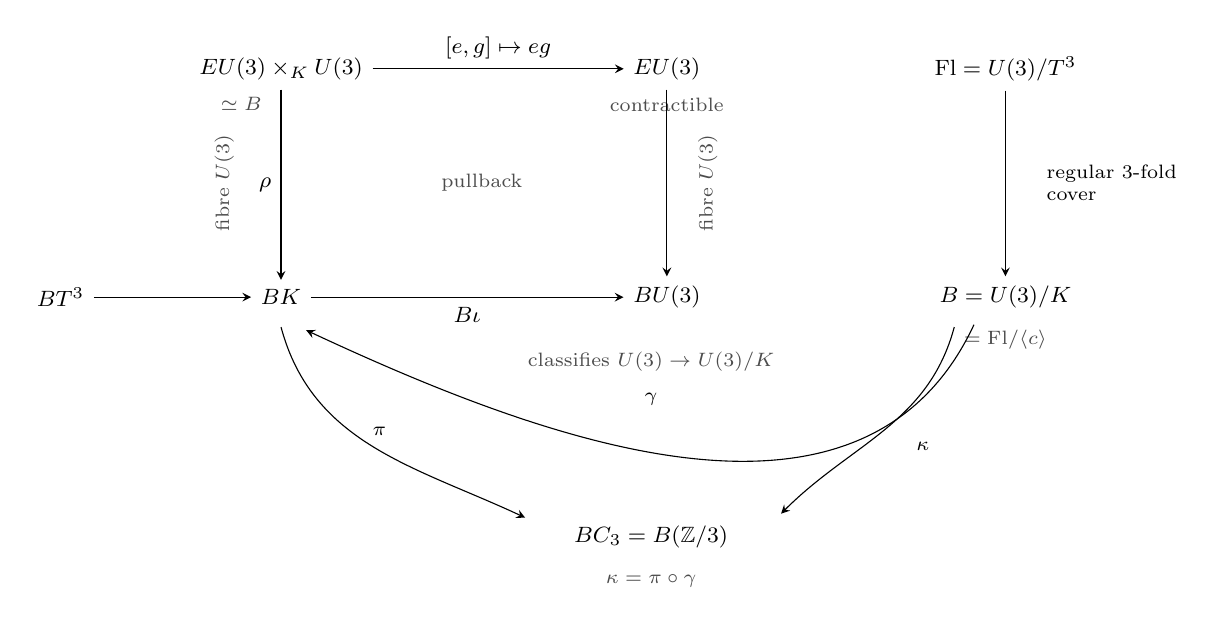
\begin{tikzpicture}[>=stealth, every node/.style={font=\footnotesize}]
  
  \node (E) at (0.3,3.3) {$EU(3)\times_K U(3)$};
  \node[anchor=east, font=\scriptsize, text=gray!60!black] at (0.18,2.86) {$\simeq B$};
  \node (F) at (5.2,3.3) {$EU(3)$};
  \node[font=\scriptsize, text=gray!60!black] at (5.2,2.84) {contractible};
  \node (G) at (0.3,0.4) {$BK$};
  \node (H) at (5.2,0.4) {$BU(3)$};
  \draw[->] (E) -- (F) node[midway, above] {$[e,g]\mapsto eg$};
  \draw[->] (E) -- (G) node[midway, left] {$\rho$};
  \draw[->] (F) -- (H);
  \draw[->] (G) -- (H) node[midway, below] {$B\iota$};
  \node[font=\scriptsize, rotate=90, text=gray!60!black] at (-0.42,1.85) {fibre $U(3)$};
  \node[font=\scriptsize, rotate=90, text=gray!60!black] at (5.72,1.85) {fibre $U(3)$};
  \node[font=\scriptsize, text=gray!60!black] at (2.85,1.85) {pullback};
  
  \node (FL) at (9.5,3.3) {$\mathrm{Fl}=U(3)/T^3$};
  \node (BN) at (9.5,0.4) {$B=U(3)/K$};
  \node[font=\scriptsize, text=gray!60!black] at (9.5,-0.14) {$=\mathrm{Fl}/\langle c\rangle$};
  \draw[->] (FL) -- (BN);
  \node[right, font=\scriptsize, align=left] at (9.9,1.85) {regular $3$-fold\\cover};
  \draw[->] (9.1,0.05) to[out=245,in=335] (0.62,-0.02);
  \node[font=\scriptsize] at (5.0,-0.9) {$\gamma$};
  \node[font=\scriptsize, text=gray!60!black] at (5.0,-0.42) {classifies $U(3)\to U(3)/K$};
  \node (BT) at (-2.5,0.4) {$BT^3$};
  \draw[->] (BT) -- (G);
  \node (BC) at (5.0,-2.65) {$BC_3=B(\mathbb Z/3)$};
  \draw[->] (0.3,0.02) to[out=285,in=155] (3.4,-2.4);
  \node[font=\scriptsize] at (1.55,-1.3) {$\pi$};
  \draw[->] (8.85,0.02) to[out=255,in=45] (6.65,-2.35);
  \node[font=\scriptsize] at (8.45,-1.5) {$\kappa$};
  \node[font=\scriptsize, text=gray!60!black] at (5.0,-3.2) {$\kappa=\pi\circ\gamma$};
\end{tikzpicture}
\caption{The spaces and maps of the proof of Proposition~\ref{prop:cupsquare}. Left: the Borel bundle of Step~1, a fibre bundle with fibre $U(3)$, total space $EU(3)\times_KU(3)$ homotopy equivalent to $B$, and base $BK$; it is the pullback of the universal bundle $U(3)\to EU(3)\to BU(3)$ along $B\iota\colon BK\to BU(3)$, with $[e,g]\mapsto eg$ on top and $BK=EC_3\times_{C_3}BT^3$ as in Step~2. Right: the homogeneous models of Step~0, the flag manifold $\mathrm{Fl}=U(3)/T^3$ and the quotient $B=U(3)/K=\mathrm{Fl}/\langle c\rangle$ under the regular three-fold cover with deck group $\langle c\rangle\cong\mathbb Z/3$, together with the classifying maps of Step~6: $\gamma$ classifies the principal $K$-bundle $U(3)\to U(3)/K$, $\pi$ is the quotient $BK\to BC_3$, and $\kappa=\pi\circ\gamma$ classifies the cover. The arrow $BT^3\to BK$ is the fibre of the fibration of Step~2. Under the identification of the total space with $B$, the projection $\rho$ equals $\gamma$; the deck transformation $c$ acts by right multiplication by the permutation matrix $\sigma$, and $K=T^3\rtimes\langle\sigma\rangle$ (Step~0).}
\label{fig:flag-fibration}
\end{figure}

\begin{proposition}[The cup square on the flag quotient]
\label{prop:cupsquare}
Keep the notation of the proof of Theorem~\ref{thm:equal-basis}: in
particular $B=\mathrm{Fl}/\langle c\rangle$ is the qutrit flag quotient,
$\kappa\colon B\to B(\mathbb Z/3)$ classifies the regular cover, and
$x=c_1(L)=\kappa^*(u)\in H^2(B;\mathbb Z)$, where $u$ generates
$H^2(B(\mathbb Z/3);\mathbb Z)\cong\mathbb Z/3$. Then
\[
x^2\ \ne\ 0\qquad\text{in }H^4(B;\mathbb Z),
\]
and, more precisely,
\[
H^k(B;\mathbb Z)\ =\ \bigl(\mathbb Z,\ 0,\ \mathbb Z/3,\ \mathbb Z/3,\
\mathbb Z/3,\ \mathbb Z/3,\ \mathbb Z\bigr)\qquad(k=0,\dots,6),
\]
with $x$ generating $H^2$, $x^2$ generating $H^4$, and
$H^6(B;\mathbb Z)\cong\mathbb Z$, in which the discriminant class is twice a
generator.
\end{proposition}

\begin{proof}
The proof runs the Serre spectral sequence of the Borel fibration
$U(3)\to B\to B\bigl(T^3\rtimes\langle\sigma\rangle\bigr)$ with integral
coefficients, in the spirit of the transgression computations used for the
unordered flag quotients in Ref.~\cite{GuerraJana2025} but lifted to the
integral layer. It is self-contained apart from three classical inputs,
each cited at the point of use: the cohomology of the flag manifold and of
$BU(3)$, Borel's transgression computation, and the cyclic cohomology of
finite modules.

The computation is organised in seven steps, and Figure~\ref{fig:flag-fibration} records the spaces and the maps used throughout. Step~0 trades the quotient description $B=\mathrm{Fl}/\langle c\rangle$ for the homogeneous-space model $B=U(3)/K$. Step~1 replaces the cover by the Borel fibration with fibre $U(3)$ and reduces the differentials of its Serre spectral sequence to the Chern classes of the inclusion $\iota\colon K\hookrightarrow U(3)$, extended by the Leibniz rule. Steps~2--4 prepare the $E_2$-page: the integral cohomology of $BK$ in Step~2, the product rule for the torsion class $\tau$ in Step~3, and the pinning of the three transgression constants through the splitting section in Step~4. The crux is Step~5, in total degree four: the incoming images kill the free summands and the fibre class $z_1z_3$, but the torsion class $\tau^2$ survives, and this survival, transferred by the edge homomorphism in Step~6, is the assertion $x^2\ne0$. Step~7 completes the remaining degrees and exhibits the discriminant as twice a generator of the top class.

\emph{Step 0 (the homogeneous-space model).} Realise
$\mathrm{Fl}=U(3)/T^3$, where $T^3\subset U(3)$ is the diagonal torus: a
flag is the ordered triple of lines spanned by the columns of a unitary
matrix $g$, and two matrices span the same triple iff they differ by right
multiplication by an element of $T^3$. Under this identification the deck
transformation $c$ is right multiplication by the permutation matrix
$\sigma$ of the cycle $(123)$, which normalises $T^3$; hence the orbits of
$\langle c\rangle$ are exactly the right cosets of the subgroup
$K:=T^3\rtimes\langle\sigma\rangle\subset U(3)$ of cyclic monomial
matrices, and $B=U(3)/K$.

\emph{Step 1 (the fibration and its transgressions).} Let $EU(3)$ be the
contractible free right $U(3)$-space. Left multiplication makes $U(3)$ a
free left $K$-space, and
\[
U(3)\ \longrightarrow\ EU(3)\times_K U(3)\ \overset{\rho}{\longrightarrow}\
BK:=EU(3)/K
\]
is a fibre bundle with fibre $U(3)$ whose total space is homotopy equivalent
to $K\backslash U(3)\cong B$ (the quotient of a free $K$-space is a model
for the associated bundle; the projection $(e,g)\mapsto g$ onto the second
factor has contractible fibres). The map $[e,g]\mapsto eg$ exhibits the
bundle as the pullback of the universal fibration $U(3)\to EU(3)\to BU(3)$
along the map $B\iota\colon BK\to BU(3)$ induced by the inclusion
$\iota\colon K\hookrightarrow U(3)$: indeed $[eg]_{U(3)}=B\iota([e]_K)$, and
on the fibres the induced map is the identity under the canonical
identifications with $U(3)$. By naturality of the Serre spectral sequence,
\[
E_2^{p,q}\ =\ H^p\bigl(BK;\ H^q(U(3);\mathbb Z)\bigr),
\]
the $K$-action on $H^*(U(3);\mathbb Z)=\Lambda(z_1,z_3,z_5)$ (one generator
$z_{2i-1}$ in each degree $2i-1$) being homotopically trivial because $U(3)$
is connected, and the differentials are the pullbacks of the universal
differentials. In the universal fibration the transgression of the primitive
class $z_{2i-1}$ is the universal Chern class $c_i$
\cite{MilnorStasheff1974,HatcherSS}; hence, extended to the exterior part by
the Leibniz rule,
\[
d_2(z_1)=\iota^*c_1,\qquad d_4(z_3)=\iota^*c_2,\qquad d_6(z_5)=\iota^*c_3,
\]
and $d_r=0$ for $r\notin\{2,4,6\}$: for odd $r$ the target sits in odd
$p$-degree, where $H^{\mathrm{odd}}(BK;\mathbb Z)=0$ by Step~3 below; for
even $r\ge8$ the source fibre-degree is $8$ or $9$, and the fibre classes
there are killed before the $E_8$-page (the classes $\sigma_1$, $\sigma_2$,
$\tau$ and the transgression values invoked here are established in
Steps~2--4 below). In fibre degree nine,
$d_2(\beta z_1z_3z_5)=\beta\sigma_1z_3z_5$ kills every class whose
coefficient survives multiplication by $\sigma_1$, and
$d_4(\tau z_1z_3z_5)=2\tau^3z_1z_5\ne0$ kills the torsion coefficients,
which annihilate $\sigma_1$. In fibre degree eight the $\sigma_1$-multiple
coefficients are $d_2$-boundaries, and the rest die under
$d_4(\beta z_3z_5)=\beta(\sigma_2+2\tau^2)z_5\ne0$: a class $\beta$ whose
$\beta\sigma_2$ is a $\sigma_1$-multiple is itself a $\sigma_1$-multiple,
rationally in the invariant module and then integrally (divisibility by
$\sigma_1=\chi_1+\chi_2+\chi_3$ is triangular in the monomials), hence a
$d_2$-boundary.

\emph{Step 2 (the cohomology of $BK$).} The semidirect structure splits, so
$BK$ is the Borel construction $EC_3\times_{C_3}BT^3$ and sits in the
fibration $BT^3\to BK\to BC_3$, whose spectral sequence has
$E_2^{p,q}=H^p\bigl(C_3;H^q(BT^3;\mathbb Z)\bigr)$ with
$H^*(BT^3;\mathbb Z)=\mathbb Z[\chi_1,\chi_2,\chi_3]$ (the tautological
characters) and $C_3$ acting by cyclic permutation of the $\chi_i$. The
monomials of each degree $d$ form free $C_3$-orbits of size three, except
the fixed monomials $(\chi_1\chi_2\chi_3)^a$ with $3a=d$; as
$\mathbb Z[C_3]$-modules the degree-$d$ part is a sum of permutation modules
--- which are acyclic for $C_3$ --- plus, when $3\mid d$, one trivial
summand. Now $H^q(BT^3)=0$ for $q$ odd, and in odd $p$-degree the entries
vanish: $H^{\mathrm{odd}}(C_3;\mathbb Z)=0$, permutation modules are
acyclic, and for the trivial summands $H^{\mathrm{odd}}(C_3;\mathbb Z
\text{-trivial})=0$. Consequently every differential lands in a zero group
--- if $r$ is even the target has odd $q$-degree, and if $r$ is odd the
target has odd, positive $p$-degree --- and the sequence collapses. The
free part, integrally, is the invariant lattice: in each degree $d$ it is
spanned by the $C_3$-orbit sums of the degree-$d$ monomials --- the fixed
monomials $(\chi_1\chi_2\chi_3)^a$ being orbits of size one --- of rank
equal to the number of orbits; the span is the whole invariant lattice,
because the monomials of an invariant polynomial occur with equal
coefficients on each orbit. Rationally, this lattice is the degree-$d$ part
of
\[
\mathbb Q[\sigma_1,\sigma_2,\sigma_3]\ \oplus\ \Delta\cdot
\mathbb Q[\sigma_1,\sigma_2,\sigma_3],
\]
where $\sigma_i=\sigma_i(\chi)$ are the elementary symmetric functions and
$\Delta=\prod_{i<j}(\chi_i-\chi_j)$ is the discriminant, invariant under the
cyclic group, with $\Delta^2$ equal to the classical discriminant polynomial
in the $\sigma_i$; the orbit counts match the monomial counts of the
displayed module, so the two rational vector spaces coincide. Integrally the
module is only a sublattice of the invariant lattice, of finite index ---
one in degrees $d\le2$, exactly the degrees in which the crux of Step~5
below works, then $2$, $2$, $4$, $8$ in degrees $3$ to $6$ --- and already in
degree three the orbit sum
$S_1=\chi_1^2\chi_2+\chi_2^2\chi_3+\chi_3^2\chi_1
=\tfrac12(\sigma_1\sigma_2-3\sigma_3+\Delta)$ is invariant but lies in the
module only after doubling. The
torsion is one $\mathbb Z/3$ in each bidegree $(2k,6a)$ with $k\ge1$; write
$\tau\in H^2(BK;\mathbb Z)\cong\mathbb Z\sigma_1\oplus\mathbb Z/3\cdot\tau$
for the class of the $(2,0)$-slot, the pullback of $u$ along
$BK\to BC_3$.

\emph{Step 3 (the torsion product rule).} Multiplication with $\tau$ is the
cup product with the generator of $H^2(C_3;\mathbb Z)$, which on the cyclic
cohomology of each module $M$ acts as the standard periodicity map
$H^0(C_3;M)\to H^2(C_3;M)$, $[f]\mapsto[f]$ \cite{Brown1982}. For the
degree-$d$ part $M=\operatorname{Sym}^d$ of $\mathbb Z[\chi]$, one has
$H^2(C_3;M)=M^{C_3}/NM$ with $N$ the norm: the invariant lattice is spanned
by the orbit sums together with the fixed monomial
$(\chi_1\chi_2\chi_3)^{d/3}$, and the norm image by the orbit sums together
with three times that monomial. Hence, for a free class $f$ of degree $d$,
\[
\tau\cdot f\ =\ \bigl[\text{coefficient of }(\chi_1\chi_2\chi_3)^{d/3}
\text{ in }f\ \bmod 3\bigr]\cdot(\text{torsion generator}),
\]
and $\tau\cdot f=0$ when $3\nmid d$. In particular $\tau\sigma_1=
\tau\sigma_2=0$ (degree not divisible by $3$) and
$\tau\sigma_1^3=0$ (the coefficient of
$\chi_1\chi_2\chi_3$ in $\sigma_1^3$ is $6$), while $\tau\sigma_3$ is the
generator of the $(2,6)$-slot --- these instances unconditional, the
$\sigma_i$ being the pinned pure classes of Step~4 below. The instance
$\tau\Delta=0$ (the graded class of the alternating $\Delta$ contains no
monomial $\chi_1\chi_2\chi_3$) is lift-dependent: the class of $\Delta$ in
$H^6(BK;\mathbb Z)$ is fixed only up to a $\tau^3$-tail, and
$\tau\cdot(\Delta+c\,\tau^3)=c\,\tau^4\ne0$ when $c\ne0$; it is not used
below. Also $\tau^k\cdot\tau^{k'}=\tau^{k+k'}\ne0$;
so $\tau^2$ is a class of order $3$ in
\[
H^4(BK;\mathbb Z)\ \cong\ \mathbb Z\sigma_1^2\ \oplus\ \mathbb Z\sigma_2\
\oplus\ \mathbb Z/3\cdot\tau^2,
\qquad
H^6(BK;\mathbb Z)\ \cong\ \mathbb Z\{A_1,\,S_1,\,S_2,\,\sigma_3\}\oplus
\mathbb Z/3\cdot\tau^3,
\]
where $A_1=\chi_1^3+\chi_2^3+\chi_3^3$ and
$S_2=\chi_1^2\chi_3+\chi_2^2\chi_1+\chi_3^2\chi_2$, with $S_1$ as in
Step~2; the two orbit sums satisfy $S_1+S_2=\sigma_1\sigma_2-3\sigma_3$ and
$S_1-S_2=\Delta$, and the symmetric-function module of Step~2 spans an
index-two sublattice of this free part, the four orbit sums generating it
exactly. The odd cohomology $H^{\mathrm{odd}}(BK;\mathbb Z)$ vanishes, as the
collapse argument shows.

\emph{Step 4 (the transgression values).} The restrictions to the fibre
$BT^3\subset BK$ are the classical Chern-root identifications
$c_i\mapsto\sigma_i(\chi)$ \cite{MilnorStasheff1974}; hence
$\iota^*c_1=\sigma_1+b\,\tau$, $\iota^*c_2=\sigma_2+\varepsilon\tau^2$
and $\iota^*c_3=\sigma_3+\varepsilon'\tau^3$ with
$b,\varepsilon,\varepsilon'\in\mathbb Z/3$ (the restriction to the fibre
pins only the free components: the torsion restricts to zero, and the
$(0,2)$-slot is $\mathbb Z\sigma_1$). The constants are pinned by the
splitting $s\colon BC_3\to BK$ of the projection $BK\to BC_3$ (the
semidirect product splits through $\sigma\mapsto(1;\sigma)$): the composite
$BC_3\to BK\overset{B\iota}{\to}BU(3)$ classifies the $K$-representation
$\sigma\mapsto$ the permutation matrix, that is, the regular representation
$1\oplus\omega\oplus\omega^2$ of $C_3$, whose Chern classes in
$H^*(BC_3;\mathbb Z)=\mathbb Z[u]/(3u)$ are $c_1=3u=0$, $c_2=2u^2$,
$c_3=0$. On the other hand $s^*$ annihilates every class of positive fibre
degree --- restricting the fibration $BT^3\to BK\to BC_3$ along $s$ gives
the fibration with fibre a point over $BC_3$, and on the $E_2$ pages the
$q>0$ slots map to zero --- while $s^*(\tau^2)=u^2$ and
$s^*(\tau^3)=u^3$. Hence $0=s^*(\iota^*c_1)=s^*(\sigma_1+b\,\tau)=bu$
(as $s^*\sigma_1=0$, the class $\sigma_1$ having positive fibre degree,
and $s^*\tau=u$, $s$ being a section of the projection whose pullback
class $\tau$ is), so $b=0$; and $2u^2=s^*(\iota^*c_2)=\varepsilon u^2$
and $0=\varepsilon'u^3$, so
\[
d_2(z_1)=\sigma_1,\qquad d_4(z_3)=\sigma_2+2\tau^2,\qquad
d_6(z_5)=\sigma_3 .
\]

\emph{Step 5 (the run, total degree four).} On
$E_2=H^*(BK;\mathbb Z)\otimes\Lambda(z_1,z_3,z_5)$ the three
transgressions, extended by the Leibniz rule, determine the whole
differential. In total degree four the terms are
$E_2^{4,0}=\mathbb Z\sigma_1^2\oplus\mathbb Z\sigma_2\oplus\mathbb
Z/3\cdot\tau^2$, $E_2^{3,1}=E_2^{1,3}=0$ (odd cohomology of $BK$),
$E_2^{2,2}=0$ (the exterior algebra $\Lambda(z_1,z_3,z_5)$ has no class of
degree two), and $E_2^{0,4}=\mathbb Z\cdot z_1z_3$. The incoming images into the $(4,0)$
slot are $d_2(\sigma_1z_1)=\sigma_1^2$ and $d_4(z_3)=\sigma_2+2\tau^2$,
while $d_2(z_1z_3)=\sigma_1z_3\ne0$ kills the $z_1z_3$ class. The class
$\tau^2$ has order three. Quotient out the direct summand
$\mathbb Z\sigma_1^2$ first --- a quotient by a direct summand leaves both
the class of $\tau^2$ and the complementary summand unchanged --- after
which the $(4,0)$-term is $\mathbb Z\sigma_2\oplus\mathbb Z/3\cdot\tau^2$
with the single incoming relation $\sigma_2+2\tau^2$, a class of infinite
order (its free component $\sigma_2$ is nonzero); an element of order
three never lies in the subgroup generated by an infinite-order class.
Consequently the class of
$\tau^2$ is nonzero in
\[
E_\infty^{4,0}\ =\ \bigl(\mathbb Z\sigma_2\oplus\mathbb Z/3\cdot\tau^2\bigr)
\big/\langle\sigma_2+2\tau^2\rangle\ \cong\ \mathbb Z/3,
\]
and, no other term of total degree four contributing,
$H^4(B;\mathbb Z)\cong\mathbb Z/3$.

\emph{Step 6 (the edge).} The edge homomorphism of the Serre spectral
sequence of a fibration, from the base cohomology to the total-space
cohomology, is the pullback along the projection
\cite{Brown1982,HatcherSS}. Under the identification of the total space
$EU(3)\times_KU(3)$ with $B$, the projection $\rho([e,g])=[e]$ is the
classifying map $\gamma\colon B\to BK$ of the principal $K$-bundle
$U(3)\to U(3)/K=B$ (the identification passes through the inversion
$K\backslash U(3)\cong U(3)/K$, so a different deck convention could at
worst flip a sign, $x=\pm\gamma^*(\tau)$; nothing below depends on the
choice, the sign squaring away in $x^2=\gamma^*(\tau^2)$). The intermediate
cover $\mathrm{Fl}=U(3)/T^3\to B$ is
the quotient of that bundle by the normal subgroup $T^3$, hence is
classified by the composite $\pi\circ\gamma$, where $\pi\colon BK\to BC_3$
is the quotient; since that cover is the regular cover classified by
$\kappa$, we have $\kappa=\pi\circ\gamma$, and therefore
\[
x\ =\ \kappa^*(u)\ =\ \gamma^*(\tau),
\qquad
x^2\ =\ \gamma^*(\tau^2)\ =\ \bigl[\tau^2\bigr]\ \ne\ 0,
\]
the last equality being the surviving class of Step 5. This proves the first
assertion.

\emph{Step 7 (the remaining degrees).} Total degree two: the incoming image
into $(2,0)$ is $d_2(z_1)=\sigma_1$, so
$H^2(B)\cong(\mathbb Z\sigma_1\oplus\mathbb Z/3\cdot\tau)/\langle\sigma_1
\rangle\cong\mathbb Z/3$, generated by the edge image
$\gamma^*(\tau)=x$. Total degree three: on
$E_2^{2,1}=\mathbb Z\sigma_1z_1\oplus\mathbb Z/3\cdot\tau z_1$ one has
$d_2(\sigma_1z_1)=\sigma_1^2\ne0$ while $d_2(\tau z_1)=\tau\sigma_1=0$, and
$E_2^{0,3}=\mathbb Z\cdot z_3$ is killed by $d_4(z_3)\ne0$; hence
$H^3(B)\cong\mathbb Z/3\cdot\langle\tau z_1\rangle$. Total degree five: on
$E_2^{4,1}=\mathbb Z\sigma_2z_1\oplus\mathbb Z\sigma_1^2z_1\oplus\mathbb
Z/3\cdot\tau^2z_1$ the free classes die under $d_2$
($\sigma_1\sigma_2$, $\sigma_1^3$) while $d_2(\tau^2z_1)=\tau^2\sigma_1=0$;
the class $\tau z_3\in E_2^{2,3}$ dies under $d_4(\tau z_3)=
\tau(\sigma_2+2\tau^2)=2\tau^3\ne0$ (Step 3), and $z_5$ dies under
$d_6(z_5)=\sigma_3$; hence $H^5(B)\cong\mathbb Z/3\cdot\langle\tau^2z_1
\rangle$. Total degree six: the incoming images into $(6,0)$ are
$\sigma_1\sigma_2$ and $\sigma_1^3$ (from $d_2$), $2\tau^3$ (from $d_4$),
and $\sigma_3$ (from $d_6$), so, running the quotient on the orbit-sum
lattice of Step~3,
\[
H^6(B;\mathbb Z)\ \cong\ \bigl(\mathbb Z\{A_1,S_1,S_2,\sigma_3\}\oplus
\mathbb Z/3\cdot\tau^3\bigr)\big/\langle\sigma_1^3,\ \sigma_1\sigma_2,\
2\tau^3,\ \sigma_3\rangle\ \cong\ \mathbb Z\cdot\langle S_1\rangle,
\]
using $\sigma_1\sigma_2=S_1+S_2+3\sigma_3$ and
$\sigma_1^3=A_1+3(S_1+S_2)+6\sigma_3$: the relations kill $\sigma_3$, then
$S_1+S_2$, then $A_1$ (each substituting into the next), the torsion class
$\tau^3$ dies because $2\tau^3=0$ forces it (two is invertible modulo
three) --- taking with it the $\tau^3$-tail ambiguity of the orbit-sum
lifts (Step~3), so that the quotient and the discriminant's position in it
are lift-independent --- and the top class is the orbit sum $S_1$, in which
the discriminant
$\Delta=S_1-S_2=2S_1$ is twice a generator --- consistently with the
rational cohomology $H^*(B;\mathbb Q)=\mathbb Q\oplus\mathbb Q\cdot
\bar\Delta$, read off from the invariant theory of Step~2, where two is
invertible and the discriminant class does generate. The mixed exterior terms die
transversally ($d_2(z_1z_3)=\sigma_1z_3$, $d_2(z_1z_5)=\sigma_1z_5$,
$d_4(\tau z_1z_3)=2\tau^3z_1$), completing the tuple.
\end{proof}

\begin{lemma}[Cohomology of the qutrit flag quotient in degrees three and four]
\label{lem:flag-cohomology}
Keep the notation of the proof of Theorem~\ref{thm:equal-basis}:
$B=\mathrm{Fl}/\langle c\rangle$ is the quotient of the qutrit flag manifold by
the cyclic shift, $\kappa\colon B\to B(\mathbb Z/3)$ classifies the regular
cover, $L\to B$ is the complex line bundle attached to the character
$c\mapsto\omega$, and $x=c_1(L)=\kappa^*(u)$, where $u$ generates
$H^2(B(\mathbb Z/3);\mathbb Z)\cong\mathbb Z/3$. Then
\[
H^3(B;\mathbb Z)\ \cong\ \mathbb Z/3,
\qquad
H^4(B;\mathbb Z)\ \cong\ \mathbb Z/3,
\]
and $x^2=\kappa^*(u^2)$ generates $H^4(B;\mathbb Z)$; in particular $x^2\ne0$.
\end{lemma}

\begin{proof}
The $E_2$ page of the Cartan--Leray spectral sequence of the free cover
$\pi\colon\mathrm{Fl}\to B$,
\[
E_2^{p,q}=H^p\bigl(\mathbb Z/3;\,H^q(\mathrm{Fl};\mathbb Z)\bigr)
\ \Longrightarrow\ H^{p+q}(B;\mathbb Z),
\]
is computed exactly as in degree two. The cohomology of $\mathrm{Fl}$ is
torsion-free with Poincar\'e polynomial $1+2t^2+2t^4+t^6$ \cite{Fulton1997};
the deck transformation $c$ cyclically permutes the three tautological
line-bundle Chern classes, so it acts on
$H^2(\mathrm{Fl};\mathbb Z)\cong\mathbb Z^3/\mathbb Z(1,1,1)$ by the cyclic
permutation $P$ and on $H^4(\mathrm{Fl};\mathbb Z)\cong\mathbb Z^2$ by an
order-three matrix of trace $-1$, which has no nonzero fixed vector; also
$H^1(\mathrm{Fl};\mathbb Z)=H^3(\mathrm{Fl};\mathbb Z)=0$. For a
$\mathbb Z/3$-module $M$ with generator action $T$ and norm $N=1+T+T^2$, the
group cohomology in positive degrees is $H^{2k}(\mathbb Z/3;M)=M^{T}/NM$ and
$H^{2k+1}(\mathbb Z/3;M)=\ker N/(T-1)M$ \cite{Brown1982}. On
$M=H^2(\mathrm{Fl};\mathbb Z)$ the norm vanishes, since $N$ sends every class
to a multiple of $\mathbb Z(1,1,1)$; the invariants $M^{P}$ vanish by the
argument of the proof of Theorem~\ref{thm:equal-basis} ($3k=0$ forces $k=0$);
and $(P-1)M$ is the image of the sum-zero sublattice
$\{(a,b,c):a+b+c=0\}$ of $\mathbb Z^3$, which together with $\mathbb Z(1,1,1)$
spans a sublattice of index three. Consequently
\[
E_2^{1,2}=\ker N/(P-1)M\ \cong\ \mathbb Z/3
\]
is the only nonzero term of total degree three, and
\[
E_2^{4,0}=H^4(\mathbb Z/3;\mathbb Z)\ \cong\ \mathbb Z/3
\]
is the only nonzero term of total degree four; the terms $E_2^{3,0}$,
$E_2^{3,1}$, $E_2^{1,3}$, and $E_2^{0,3}$ vanish (odd-degree cohomology of
the cyclic group with trivial coefficients, and
$H^1(\mathrm{Fl})=H^3(\mathrm{Fl})=0$), while $E_2^{2,2}=M^{P}/NM=0$ and
$E_2^{0,4}=H^4(\mathrm{Fl};\mathbb Z)^{\mathbb Z/3}=0$ by the vanishing fixed
vectors.

No differential leaves $E_r^{4,0}$ (its targets $(4+r,1-r)$ have negative
second coordinate) and none reaches $E_r^{1,2}$ (its sources have negative
first coordinate); the sources of the $d_2$ and $d_4$ entering $E^{4,0}$,
namely $E_2^{2,1}$ and $E_2^{0,3}$, vanish. The only differential that can
affect either term is therefore $d_3^{1,2}\colon E_3^{1,2}\to E_3^{4,0}$, and
since these are the only terms of their total degrees,
\[
H^3(B;\mathbb Z)\ \cong\ \ker d_3^{1,2},
\qquad
H^4(B;\mathbb Z)\ \cong\ \operatorname{coker} d_3^{1,2}.
\]
The page alone does not decide $d_3^{1,2}$: both the zero map and the
isomorphism of $\mathbb Z/3$ are consistent with every entry derived so far,
including the degree-two and top-degree identifications used in the proof of
Theorem~\ref{thm:equal-basis}. The decision between the two worlds is
supplied by Proposition~\ref{prop:cupsquare}, which proves $x^2\ne0$ by an
integral transgression computation independent of the present Cartan--Leray
page; and $x^2=\kappa^*(u^2)$ is, exactly as in degree two in the
proof of Theorem~\ref{thm:equal-basis} \cite{Brown1982}, the image of $u^2$
under the edge homomorphism $H^4(\mathbb Z/3;\mathbb Z)\to H^4(B;\mathbb Z)$,
which factors as $H^4(\mathbb Z/3;\mathbb Z)\to E_\infty^{4,0}=
\operatorname{coker}d_3^{1,2}\hookrightarrow H^4(B;\mathbb Z)$. A nonzero
image forces a nonzero cokernel, and a homomorphism
$\mathbb Z/3\to\mathbb Z/3$ with nonzero cokernel is zero: $d_3^{1,2}=0$.
Then $H^3(B;\mathbb Z)=\ker d_3^{1,2}\cong\mathbb Z/3$ and
$H^4(B;\mathbb Z)=\operatorname{coker}d_3^{1,2}\cong\mathbb Z/3$, the class
$u^2$ survives to $E_\infty^{4,0}$, and $\kappa^*(u^2)=x^2$ generates
$H^4(B;\mathbb Z)$. The independent machine computation recorded in
Remark~\ref{rem:machine-certificate} confirms the same conclusion and agrees
with the full cohomology tuple of Proposition~\ref{prop:cupsquare}.
\end{proof}

\begin{remark}[The computational verification of Lemma~\ref{lem:flag-cohomology}]
\label{rem:machine-certificate}
The proof of Lemma~\ref{lem:flag-cohomology} is analytic: its decision input
$x^2\ne0$ is Proposition~\ref{prop:cupsquare}, whose transgression
computation uses only cited classical results (the cohomology of
$U(3)$ and $BU(3)$, Borel's transgression, and the cyclic cohomology of finite
modules \cite{MilnorStasheff1974,HatcherSS,Brown1982}) plus a self-contained
invariant-theory step. An independent machine computation, described in this
remark, cross-checks the conclusion: it determines the integral homology of
$B$ directly and agrees with the full cohomology tuple of
Proposition~\ref{prop:cupsquare}.

The homology of $B$ was computed from a free
$\mathbb Z/3$-equivariant finite cellulation of $\mathrm{Fl}$ with
$14\,910$ cells, constructed on the boundary stratification of the
unistochastic region of the three-dimensional unitary group (a two-sheet book
over the stratified base, seam-subdivided). The certification consists of
exact integer arithmetic on that complex: cell counts and Euler
characteristic $\chi(\mathrm{Fl})=6=3\,\chi(B)$; $\partial^2=0$ on every
cell; the induced action $T$ satisfies $T^3=\mathrm{id}$ and
$\partial T=T\partial$; the action is free; the cover homology is the
classical one, $H_*(\mathrm{Fl})=(\mathbb Z,0,\mathbb Z^2,0,\mathbb Z^2,0,
\mathbb Z)$, with vanishing torsion at the primes $2,3,5,7$; and the orbit
complex of $B$ satisfies $\bar\partial^2=0$, from which the Smith normal
forms of the orbit boundary matrices pin every slot,
$H_*(B)=(\mathbb Z,\mathbb Z/3,\mathbb Z/3,\mathbb Z/3,\mathbb Z/3,0,\mathbb
Z)$, with the torsion exponents fixed ($H_2=H_3=H_4=\mathbb Z/3$, no
$\mathbb Z/9$ summands) and no further torsion at any prime $p\le61$. The
computation is anchored externally at four independent points: the
Poincar\'e polynomial of $\mathrm{Fl}=U(3)/U(1)^3$; $H_1(B)=\mathbb Z/3$,
which Cartan--Leray forces for any free $\mathbb Z/3$-quotient of the simply
connected $\mathrm{Fl}$; $\chi(\mathrm{Fl})=3\chi(B)$; and the palindromic
universal-coefficient ladder of $H_*(B)$. The decision logic of the lemma
--- the reading of $d_3^{1,2}$ off the certified cohomology, and the
Euler-class arithmetic of Theorem~\ref{thm:equal-basis-plane} below --- was
checked against two externally known model cases: the lens space
$L(3;1,1,1)$, where $x^2\ne0$ and $d_3^{1,2}=0$, and
$\mathbb{RP}^2\times S^2$, where $x^2=0$ and $d_3^{1,2}$ is an isomorphism;
in both, the direct homology, the spectral-sequence page, and the cup-square
computation agree.

Three qualifications remain. First, the arithmetic of
Proposition~\ref{prop:cupsquare} rests on three cited classical inputs ---
Borel's transgression computation for the universal bundle, the Chern-root
restriction, and the cyclic cohomology of finite modules --- and its
internal bookkeeping (the orbit counts, the orbit-sum invariant lattice
together with its finite index over the symmetric-function module, the
twice-a-generator position of the discriminant in the top class, the torsion
product rule, the Chern classes of the regular representation, and the
Leibniz-signed page bookkeeping, including the $D^2=0$ coherence check) is
verified by an exact-integer computation; the transgression mechanism itself
reproduces the classical cohomology on the model fibration
$SU(2)\to SU(2)/C_3\to BC_3$, where the same differential structure
($d_4(z_3)=2u^2$, the second Chern class of the regular representation)
yields $H^*(L(3;1);\mathbb Z)=
(\mathbb Z,0,\mathbb Z/3,\mathbb Z)$ with the transfer edge
$\pi^*[L]^*=3[S^3]^*$. Second, the cellulation was implemented twice
independently, the second implementation following the design specification
with different algorithms at every layer (phase measurement by column ratios
rather than a joint gauge solve, Newton inversions, sign derivation by
constraint propagation from $\partial T=T\partial$, direct $\mathbb Z/12$
elimination rather than the Chinese-remainder route, and an incremental
subgroup-order computation of the $\mathbb Z/9$ ladder); the two
implementations agree on every input datum and on the homology tuple, and
the convention data of the construction is forced by the certification (each
falsified variant breaks either the equivariance certificate or the orbit
homology). Third, the geometric identification with the flag quotient is
warranted by the construction lineage and the certification, not by an
explicit diffeomorphism, and the prime scan is finite, covering $p\le 31$
across the two implementations. The premise of
Lemma~\ref{lem:flag-cohomology} is thus carried by three mutually
independent routes --- the analytic derivation, the cellulation, and its
independent re-implementation --- which agree on the tuple. The code and
the full transcripts of both computations are available in the public
repository.\footnote{\url{https://github.com/MIKEAA2020/channel-supp-augmented}}
\end{remark}

\begin{remark}[The neighbouring flag-quotient literature]
\label{rem:flag-literature}
The quotient $B=\mathrm{Fl}/\langle c\rangle$ of Lemma~\ref{lem:flag-cohomology}
sits next to an active line on the cohomology of quotients of flag manifolds
and their applications. Guerra and Jana~\cite{GuerraJana2025} determine the
cohomology of the complete unordered flag manifolds
$\mathrm{Fl}_n(\mathbb C)/\Sigma_n$ and $\mathrm{Fl}_n(\mathbb R)/\Sigma_n$
--- homological stability, closed forms for the stable rings, and an
algorithmic procedure for the unstable additive cohomology --- and, with
Maiti~\cite{GuerraJanaMaiti2025}, compute the mod-$2$ cohomology of the
low-dimensional real unordered flag manifolds, improving the known estimates
of the number of Auerbach bases of small-dimensional normed spaces; this is
the line opened by Weber and Wojciechowski's Lusternik--Schnirelmann-category
estimate via real flag varieties~\cite{WeberWojciechowski2017}, together with
the cup-length computations of Korba{\v s} and L\"orinc~\cite{KorbasLorinc2003}
and Matszangosz's algorithm for the integer cohomology of real partial flag
manifolds~\cite{Matszangosz2021}. The classical backdrop of the antipodal
arguments specialised here to $\mathbb Z/3$ is the cyclic-group
Borsuk--Ulam literature, from the simple proof for
$\mathbb Z_p$-actions~\cite{Singh2010} to the connective $K$-theory version
for cyclic $p$-groups~\cite{Crabb2022}. The differentiation is precise. That
programme treats the \emph{symmetric-group} quotients, with \emph{field}
coefficients, in the service of Auerbach-basis counting; the present premise
concerns the \emph{cyclic} intermediate quotient
$\mathrm{Fl}/\langle c\rangle$, with \emph{integral} coefficients and the
$3$-torsion exponents pinned, in the service of the equal-value-basis and
compression-width chain. The derivation of Proposition~\ref{prop:cupsquare} is the
integral lift of the transgression route that the algorithmic procedure of
Ref.~\cite{GuerraJana2025} inspires: the same fibration comparison and
Chern-class transgressions, with the invariant-theoretic input replacing the
field-coefficient module algebra, and the torsion-survival argument of
Step~5 handling the integral $3$-torsion layer that the field-coefficient
algorithms of that programme do not address. The computational verification of
Remark~\ref{rem:machine-certificate} remains complementary to, not subsumed
by, that programme.
\end{remark}

\begin{theorem}[Equal-value bases for plane-valued maps]
\label{thm:equal-basis-plane}
Let $V$ be a three-dimensional complex Hilbert space and let
$f\colon\mathbb P(V)\to\mathbb R^2$ be continuous. Then $V$ admits an
orthonormal basis $(\psi_1,\psi_2,\psi_3)$ with
\[
f([\psi_1])\ =\ f([\psi_2])\ =\ f([\psi_3]).
\]
\end{theorem}

\begin{proof}
We adapt the proof of Theorem~\ref{thm:equal-basis}, keeping its notation
($\mathrm{Fl}$, the shift $c$, the projection $p_1$, and the quotient $B$),
and write $g=f\circ p_1\colon\mathrm{Fl}\to\mathbb R^2$,
$h=g-g\circ c\colon\mathrm{Fl}\to\mathbb R^2$, and
$H=(h,\ h\circ c)\colon\mathrm{Fl}\to\mathbb R^4$. The telescoping identity
$h+h\circ c+h\circ c^2\equiv0$ yields
\[
H\circ c=T\,H,
\qquad
T=\begin{pmatrix}0&I_2\\-I_2&-I_2\end{pmatrix},
\]
namely $T=T_1\otimes I_2$ with the two-by-two matrix $T_1$ of the proof of
Theorem~\ref{thm:equal-basis}; since $T_1=SRS^{-1}$ with $S$ real invertible
and $R$ the plane rotation by $2\pi/3$, we have
$T=(S\otimes I_2)(R\otimes I_2)(S\otimes I_2)^{-1}$. Replacing $H$ by
$(S\otimes I_2)^{-1}H$, which does not change where $H$ vanishes, we may take
$T=R\otimes I_2$.

Suppose, for contradiction, that $H$ never vanishes. Then
$\widehat H=H/\|H\|_2\colon\mathrm{Fl}\to S^3$ is well defined (the map
$R\otimes I_2$ is orthogonal, so $\|H\circ c\|_2=\|H\|_2$) and satisfies
\[
\widehat H(cx)=(R\otimes I_2)\,\widehat H(x).
\]
Write $J_R$ for the quarter-turn of the first $\mathbb R^2$ factor and put
$J=J_R\otimes I_2$, a complex structure on $\mathbb R^4$. Since
$R=\cos(2\pi/3)I_2+\sin(2\pi/3)J_R$, the map
$R\otimes I_2=\cos(2\pi/3)I_4+\sin(2\pi/3)J$ is multiplication by $\omega$
on the complex plane $(\mathbb R^4,J)\cong\mathbb C^2$. Thus $\widehat H$ is
a nowhere-vanishing continuous section of the rank-two complex vector bundle
\[
L\oplus L\ =\ \bigl(\mathrm{Fl}\times\mathbb C^2\bigr)\big/
\bigl((x,z)\sim(cx,\ \omega z)\bigr)
\ \longrightarrow\ B,
\]
the direct sum of two copies of the line bundle $L$ of the proof of
Theorem~\ref{thm:equal-basis} (the representation $z\mapsto\omega z$ of
$\mathbb Z/3$ on $\mathbb C^2$ is twice the character of $L$). A continuous
nowhere-vanishing section $s$ of an oriented real vector bundle $E$ splits
$E=\mathbb Rs\oplus E'$, and the Whitney product formula for Euler classes
\cite{MilnorStasheff1974} gives $e(E)=e(\mathbb Rs)\,e(E')=0$, since the
Euler class of a trivial line bundle vanishes. For the underlying oriented
real bundle of a complex rank-two bundle the Euler class is the second Chern
class, and by the Whitney sum formula \cite{MilnorStasheff1974},
\[
0\ =\ e(L\oplus L)\ =\ c_2(L\oplus L)\ =\ c_1(L)\,c_1(L)\ =\ x^2,
\]
contradicting $x^2\ne0$ (Lemma~\ref{lem:flag-cohomology}).

So $H$ vanishes at some $x\in\mathrm{Fl}$: $h(x)=0$ and $h(cx)=0$, that is,
$g(x)=g(cx)=g(c^2x)$; the three lines of the flag $x$ form an orthonormal
basis of $V$ on which $f$ takes one common value.
\end{proof}

\begin{theorem}[Second latent dimension of the state space for $d_B\ge3$]
\label{thm:state-d2}
Assume $d_A=1$ and $d_B\ge3$. Then the one-outcome body --- the state space
$\mathcal D(B)$ under the identification of the input-independent case ---
satisfies
\[
\delta_{2,\mathrm{inst}}^{\diamond}(\mathbb C,B)\ \ge\ \frac43,
\]
with equality at $d_B=3$; for $d_B\ge4$ the width lies in
$[\,4/3,\ 2(1-1/d_B)\,]$.
\end{theorem}

\begin{proof}
Let $f\colon\Inst_1(\mathbb C,B)\to\mathbb R^2$ be a continuous encoder and
$g\colon\mathbb R^2\to\Inst_1(\mathbb C,B)$ a decoder, let $V\subseteq B$ be
a three-dimensional subspace, and restrict $f$ to the pure states of $V$.
Theorem~\ref{thm:equal-basis-plane} supplies an orthonormal basis
$(\psi_1,\psi_2,\psi_3)$ of $V$ with $f(\psi_i\psi_i^*)=t\in\mathbb R^2$ for
$i=1,2,3$. Write $c=g(t)$, a state: $c\succeq0$ and $\Tr c=1$. Then, exactly
as in the proof of Theorem~\ref{thm:state-nonflat},
\[
\sum_{i=1}^3\langle\psi_i|c|\psi_i\rangle
=\Tr(cP_V)\ \le\ \Tr c=1,
\]
because $c\succeq0$ and $P_V\preceq I$; hence some $i$ has
$\langle\psi_i|c|\psi_i\rangle\le\tfrac13$. For that $i$ the matrix
$X=\psi_i\psi_i^*-c$ is Hermitian and traceless, so
\[
\|X\|_1=2\,\Tr X_+\ \ge\ 2\Bigl(1-\langle\psi_i|c|\psi_i\rangle\Bigr)
\ \ge\ \frac43.
\]
Every encoder/decoder pair at latent dimension two therefore suffers
worst-case error at least $4/3$. The upper bounds are those of the proof of
Theorem~\ref{thm:state-nonflat}: monotonicity of the widths in the latent
dimension (Proposition~\ref{prop:monotonicity}) gives $\delta_2\le\delta_1$,
with $\delta_1\le\delta_0=R_1=2(1-1/d_B)$ the constant-code value of
Corollary~\ref{cor:constant-code} at $n=1$; at $d_B=3$ this gives
$\delta_2\le4/3$, and at $d_B\ge4$ the bracket $[\,4/3,\ 2(1-1/d_B)\,]$.
\end{proof}

\begin{remark}[Decoder scope at the second index]
\label{rem:affine-scope-2}
The decoder-scope discussion of Remark~\ref{rem:affine-scope} applies
verbatim at the second index: at $d_B=3$ the projection $P_V$ is the
identity, so the bound of Theorem~\ref{thm:state-d2} survives even decoders
valued in the ambient affine space (Remark~\ref{rem:decoder-codomain}); at
$d_B\ge4$ the inequality $\Tr(cP_V)\le\Tr c$ uses $c\succeq0$, so the bound
is proved for the width as defined, with instrument-valued decoders.
\end{remark}

\begin{corollary}[Complete bottom-width classification for $d_A=1$]
\label{cor:bottom-dichotomy}
Assume $d_A=1$ and $nd_B>2$. Then
\[
\delta_{1,\mathrm{inst}}^{\diamond}(\mathbb C,B)=1
\qquad\Longleftrightarrow\qquad
nd_B\le4\ \text{ and }\ d_B\le2,
\]
and $\delta_{1,\mathrm{inst}}^{\diamond}(\mathbb C,B)\ge4/3$ in every other case.
The value $4/3$ is exact at the three instances $(n,d_B)=(5,1)$, $(1,3)$, and
$(2,3)$; the one-outcome
ququart lies in $[4/3,3/2]$, and so does the classical six-outcome simplex.
\end{corollary}

\begin{proof}
The flat cases with $nd_B\le4$ and $d_B\le2$ are $\{(2,1),(3,1),(4,1)\}$ (the
bases of Theorem~\ref{thm:flat-half}), $(1,2)$ (the collapse,
Theorem~\ref{thm:collapse}), and $(2,2)$ (the mass-split encoder,
Proposition~\ref{prop:mass-split}(ii) at $d_B=2$). In every other case:
$d_B=1$ with $n\ge5$, and $d_B=2$ with $n\ge3$, are covered by
Theorem~\ref{thm:nonflat-d1} with $q=3$ ($nd_B\ge5$); $n=1$ with $d_B\ge3$ is
Theorem~\ref{thm:state-nonflat}; $n\ge2$ with $d_B\ge3$ has $nd_B\ge6\ge5$ and is
covered by Theorem~\ref{thm:nonflat-d1} again. The exact values are
Corollary~\ref{cor:exact-d1} at $(5,1)$, Theorem~\ref{thm:state-nonflat} at
$(1,3)$, and Theorem~\ref{thm:mass-exact} at $(2,3)$ ($d_B=3$ is a prime power);
the stated brackets are the constant-code value at $(1,4)$ and
Proposition~\ref{prop:pair-d1} at $n=6$.
\end{proof}

\begin{lemma}[Concentration gate]
\label{lem:slice-gate}
Assume $d_A=1$ and $d_B\ge2$. If an $n$-outcome instance is flat at some
$r\ge1$, $\delta_{r,\mathrm{inst}}^{\diamond}(\mathbb C,B)=1$, then the
one-outcome body at the same output dimension satisfies
$\delta_{r,\mathrm{inst}}^{\diamond}\bigl(\Inst_1(\mathbb C,B)\bigr)\le1$. In
particular every flat instance at output dimension $d_B$ requires the
state-space width $\delta_r\bigl(\mathcal D(B)\bigr)\le1$ at the same latent
dimension $r$.
\end{lemma}

\begin{proof}
Let $(f,g)$ achieve worst-case error at most $1$ on $\Inst_n(\mathbb C,B)$ and
let $\jmath\colon\Inst_1(\mathbb C,B)\to\Inst_n(\mathbb C,B)$ place the whole
mass in the first slot, $\jmath(\rho)=(\rho,0,\dots,0)$; then
$f\circ\jmath$ is a continuous encoder into $\mathbb R^r$. Write
$g(t)=\bigl(g_1(t),\dots,g_n(t)\bigr)$ and fix a state
$\sigma_0\in\mathcal D(B)$. The blocks of $g(t)$ are positive semidefinite with
$\sum_k\Tr g_k(t)=1$, so the slack $1-\Tr g_1(t)=\sum_{k\ge2}\Tr g_k(t)$ is
nonnegative, and the padded first block
\[
\bar g_1(t)\ :=\ g_1(t)+\bigl(1-\Tr g_1(t)\bigr)\,\sigma_0
\]
is again a state, so $\bar g_1\colon\mathbb R^r\to\Inst_1(\mathbb C,B)$ is a
decoder for the one-outcome body. For every $\rho\in\Inst_1(\mathbb C,B)$,
using $\|Y\|_1=\Tr Y$ for positive semidefinite $Y$,
\[
\bigl\|\rho-\bar g_1(f(\jmath\rho))\bigr\|_1
\ \le\ \bigl\|\rho-g_1(f(\jmath\rho))\bigr\|_1
+\bigl(1-\Tr g_1(f(\jmath\rho))\bigr)
\ =\ \bigl\|\jmath(\rho)-g(f(\jmath\rho))\bigr\|_{\diamond,\mathrm{inst}}
\ \le\ 1,
\]
where the middle identity reassembles the block sum: the slack
$\sum_{k\ge2}\Tr g_k$ equals the tail contribution
$\sum_{k\ge2}\|g_k\|_1$. The padded pair
$\bigl(f\circ\jmath,\ \bar g_1\bigr)$ is thus an encoder/decoder pair for the
one-outcome body at latent dimension $r$ with worst-case error at most $1$,
which proves the first claim; the second claim is the identification of
$\Inst_1(\mathbb C,B)$ with $\mathcal D(B)$ carrying the trace norm.
\end{proof}

\begin{remark}[Status of the flat-width problem for $d_A=1$]
\label{rem:flat-status}
The problem is governed by the flag-coordinate count $nd_B$, with a complete answer
at the bottom index. On the obstruction side,
the median matching bound at $r=1$ (Theorem~\ref{thm:nonflat-d1}), the topological
Tverberg bound at every $r\ge2$ (Theorem~\ref{thm:tverberg}), and the
equal-value-basis theorem (Theorem~\ref{thm:equal-basis}) combine into
Corollary~\ref{cor:flat-fails}: $\delta_r\ge4/3$ whenever $nd_B\ge2r+3$, with the
sharpening $\delta_r\ge2(q-1)/q$ available whenever $2q-1\le nd_B$ at $r=1$ (all $q$)
or $(q-1)(r+1)\le nd_B-1$ at $r\ge2$ ($q$ a prime power). Note that the median
obstruction requires five \emph{coordinates}, not five outcomes: a single slot with
$d_B\ge5$ basis flags already triggers it, which is why the one-outcome state space
and few-outcome quantum bodies are covered. On the constructive side:
the complete classical dichotomy $\delta_r=1\iff n\le2r+2$
(Corollary~\ref{cor:classical-dichotomy}); the complete qubit dichotomy
$\delta_r=1\iff r\ge n-1$ (Corollary~\ref{cor:qubit-dichotomy}, improving the
two-sector pinching threshold $nQ_2(2)-1=2n-1$); the exact boundary values $4/3$ (Corollary~\ref{cor:exact-d1}); and the exact
value $2(1-1/d_B)$ at $r=n-1$ for prime-power $d_B$ (Theorem~\ref{thm:mass-exact}).
At the bottom index the classification is complete
(Corollary~\ref{cor:bottom-dichotomy}): $\delta_1=1$ exactly on
$\{(n,d_B):n\le4,\ d_B=1\}\cup\{(1,2),(2,2)\}$ (the latter by the mass-split encoder
at $n=2$) and $\delta_1\ge4/3$ on every other input-independent body; the one-outcome
state spaces are non-flat, the qutrit having $\delta_1=4/3$ exactly and the ququart lies in
$[4/3,\,3/2]$ (Theorem~\ref{thm:state-nonflat}). For $d_B\ge3$ above the diagonal at
$r\ge2$, flatness is certified from
$r\ge nQ_2(d_B)-1$ (Theorem~\ref{thm:pinching}) and the mass-split encoder gives
$\delta_{n-1}\le2(1-1/d_B)$; the open range is $r\ge3$ with $(nd_B-3)/2<r<nQ_2(d_B)-1$: by the concentration gate (Lemma~\ref{lem:slice-gate}) every flat instance at output dimension $d_B$ requires $\delta_r\bigl(\mathcal D(B)\bigr)\le1$, and at $r=2$ this requirement fails for every $d_B\ge3$ --- $\delta_2\bigl(\mathcal D(B)\bigr)\ge4/3$, exactly $4/3$ at the qutrit (Theorem~\ref{thm:state-d2}) --- so no $d_B\ge3$ instance is flat at the second index and the gating unknowns are the state-space widths from the third index on. For $d_B=2$
below the diagonal, the mass-split encoder with $k\ge1$ undecoded tail slots gives
$\delta_{n-k}\le2-1/k$ (decode the tail blocks as $\big((1-s)/k\big)I_B/2$, where $s$
is the decoded head mass; each tail block then errs by at most its trace plus its mass
deviation from $(1-s)/k$), so the sub-boundary qubit widths lie in $[4/3,\,2-1/k]$.
Conjecture~\ref{con:coord-flat} states the expected complete
picture.
\end{remark}

\begin{conjecture}[Coordinate dichotomy for input-independent flat widths]
\label{con:coord-flat}
Assume $d_A=1$ and $nd_B>2$. Then
\[
\delta_{r,\mathrm{inst}}^{\diamond}(\mathbb C,B)=1
\qquad\Longleftrightarrow\qquad
nd_B\ \le\ 2r+2
\quad\text{and}\quad
\bigl(d_B\le2\ \text{or}\ r\ge3\bigr) \quad\big(1\le r\le nd_B^2-2\big).
\]
\end{conjecture}

The obstruction direction is proved for every $d_B\ge1$: $nd_B\ge2r+3$ forces
$\delta_r\ge4/3$ (Corollary~\ref{cor:flat-fails}, sharpened to $2(q-1)/q$ by Theorems
~\ref{thm:nonflat-d1} and~\ref{thm:tverberg} where a large enough $q$ is available).
The flat direction is proved for $d_B\in\{1,2\}$ (Corollaries ~\ref{cor:classical-dichotomy} and~\ref{cor:qubit-dichotomy}) and fails at $r\in\{1,2\}$ for every $d_B\ge3$ (Theorems~\ref{thm:equal-basis} and~\ref{thm:state-nonflat}, together with Theorem~\ref{thm:state-d2}). The content of the conjecture is therefore the flat direction at $d_B\ge3$ with $r\ge3$: that
$r\ge\lceil(nd_B-2)/2\rceil$ latent dimensions --- one per two flag coordinates ---
suffice for error one. This is a strong demand: the pinching constructions certify
flatness only from $nQ_2(d_B)-1$ upward, a rate of $Q_2(d_B)$ latent dimensions per
slot. But it is the exact generalisation of both proved dichotomies, and it is
consistent with the exact values of Theorem~\ref{thm:mass-exact}: for $d_B\ge3$, the
index $r=n-1$ lies strictly below the conjectured flat range (indeed $nd_B>2n$) and
there $\delta_{n-1}=2(1-1/d_B)>1$.

Figure~\ref{fig:flat-regimes} displays the resulting regimes. The classification admits a direct operational reading. The value $1$ is the antipodal floor: the exact antipodal profile of the input-independent case forces error at least $1$ throughout the subcritical range, so a flat width means that the topological lower bound is attained --- the latent dimension is as economical as the obstruction permits. The bound $\delta_r\ge4/3$ is a fixed surcharge of one third above the floor, and its mechanism is visible in the proofs of Theorems~\ref{thm:state-nonflat} and~\ref{thm:state-d2}: every continuous real function, and at the second index every continuous plane-valued map, takes a common value on some orthonormal basis (Theorems~\ref{thm:equal-basis} and~\ref{thm:equal-basis-plane}), and the decoder attached to that value under-weights one of the basis states by mass at least $2/3$, the trace norm charging twice the missing mass. At the qutrit the surcharge is exact at each of the first two latent dimensions, and it is operationally detectable: by the discrimination formula of Remark~\ref{rem:operational}, an error of $4/3$ corresponds to a single-use discrimination success probability of $5/6$, so every one- or two-dimensional code of the qutrit state space leaves some state whose coded reconstruction is distinguishable from it with probability at least $5/6$.

\begin{figure}[t]
\centering
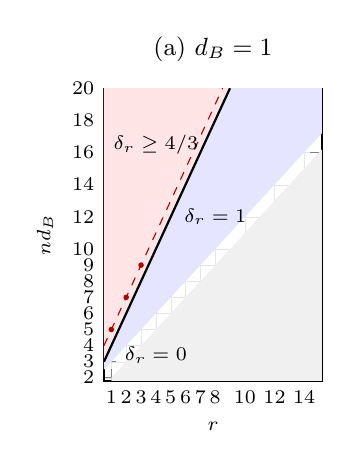
\begin{tikzpicture}
\begin{axis}[
    width=4.35cm, height=5.3cm,
    xlabel={$r$}, ylabel={$nd_B$},
    xmin=0.5, xmax=15.2, ymin=1.8, ymax=20,
    xtick={1,2,3,4,5,6,7,8,10,12,14},
    ytick={2,3,4,5,6,7,8,9,10,12,14,16,18,20},
    grid=both, grid style={line width=.1pt, draw=gray!20},
    tick label style={font=\scriptsize}, label style={font=\scriptsize},
    title={(a) $d_B=1$}, title style={font=\small}
]
\fill[gray!12] (axis cs:1,1.8) -- (axis cs:15.2,1.8) -- (axis cs:15.2,16.2) -- (axis cs:1,2) -- cycle;
\fill[blue!10] (axis cs:0.5,2.5) -- (axis cs:0.5,3) -- (axis cs:9,20) -- (axis cs:15.2,20) -- (axis cs:15.2,17.2) -- cycle;
\fill[red!10] (axis cs:0.5,3) -- (axis cs:0.5,20) -- (axis cs:9,20) -- cycle;
\draw[thick] (axis cs:0.5,3) -- (axis cs:9,20);
\draw[dashed, red!70!black] (axis cs:0.5,4) -- (axis cs:8.5,20);
\fill[red!70!black] (axis cs:1,5) circle (1.0pt);
\fill[red!70!black] (axis cs:2,7) circle (1.0pt);
\fill[red!70!black] (axis cs:3,9) circle (1.0pt);
\node[font=\scriptsize] at (axis cs:4,16.5) {$\delta_r\ge4/3$};
\node[font=\scriptsize] at (axis cs:8,12) {$\delta_r=1$};
\node[font=\scriptsize] at (axis cs:4,3.4) {$\delta_r=0$};
\end{axis}
\end{tikzpicture}
\hfil
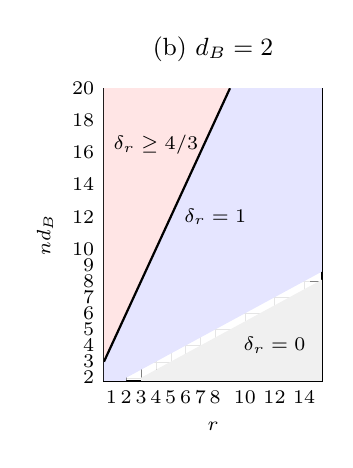
\begin{tikzpicture}
\begin{axis}[
    width=4.35cm, height=5.3cm,
    xlabel={$r$}, ylabel={$nd_B$},
    xmin=0.5, xmax=15.2, ymin=1.8, ymax=20,
    xtick={1,2,3,4,5,6,7,8,10,12,14},
    ytick={2,3,4,5,6,7,8,9,10,12,14,16,18,20},
    grid=both, grid style={line width=.1pt, draw=gray!20},
    tick label style={font=\scriptsize}, label style={font=\scriptsize},
    title={(b) $d_B=2$}, title style={font=\small}
]
\fill[gray!12] (axis cs:3,1.8) -- (axis cs:15.2,1.8) -- (axis cs:15.2,8.1) -- (axis cs:3,2) -- cycle;
\fill[blue!10] (axis cs:0.5,1.8) -- (axis cs:0.5,3) -- (axis cs:9,20) -- (axis cs:15.2,20) -- (axis cs:15.2,8.6) -- (axis cs:2,2) -- (axis cs:2,1.8) -- cycle;
\fill[red!10] (axis cs:0.5,3) -- (axis cs:0.5,20) -- (axis cs:9,20) -- cycle;
\draw[thick] (axis cs:0.5,3) -- (axis cs:9,20);
\node[font=\scriptsize] at (axis cs:4,16.5) {$\delta_r\ge4/3$};
\node[font=\scriptsize] at (axis cs:8,12) {$\delta_r=1$};
\node[font=\scriptsize] at (axis cs:12,4) {$\delta_r=0$};
\end{axis}
\end{tikzpicture}
\hfil
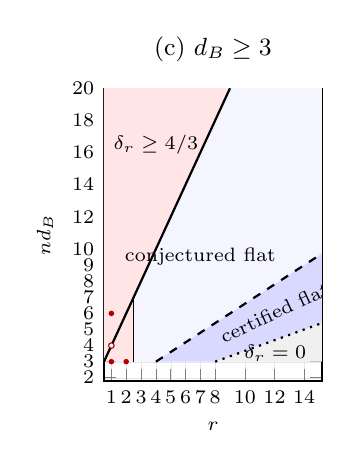
\begin{tikzpicture}
\begin{axis}[
    width=4.35cm, height=5.3cm,
    xlabel={$r$}, ylabel={$nd_B$},
    xmin=0.5, xmax=15.2, ymin=1.8, ymax=20,
    xtick={1,2,3,4,5,6,7,8,10,12,14},
    ytick={2,3,4,5,6,7,8,9,10,12,14,16,18,20},
    grid=both, grid style={line width=.1pt, draw=gray!20},
    tick label style={font=\scriptsize}, label style={font=\scriptsize},
    title={(c) $d_B\ge3$}, title style={font=\small}
]
\fill[red!10] (axis cs:0.5,3) -- (axis cs:0.5,20) -- (axis cs:9,20) -- cycle;
\fill[red!10] (axis cs:0.5,3) -- (axis cs:2.5,7) -- (axis cs:2.5,3) -- cycle;
\fill[blue!4] (axis cs:2.5,7) -- (axis cs:9,20) -- (axis cs:15.2,20) -- (axis cs:15.2,9.72) -- (axis cs:4,3) -- (axis cs:2.5,3) -- cycle;
\fill[blue!15] (axis cs:4,3) -- (axis cs:15.2,9.72) -- (axis cs:15.2,5.4) -- (axis cs:8,3) -- cycle;
\fill[gray!12] (axis cs:8,3) -- (axis cs:15.2,3) -- (axis cs:15.2,5.4) -- cycle;
\draw[thick] (axis cs:0.5,3) -- (axis cs:9,20);
\draw[dashed, thick] (axis cs:4,3) -- (axis cs:15.2,9.72);
\draw[dotted, thick] (axis cs:8,3) -- (axis cs:15.2,5.4);
\draw (axis cs:2.5,3) -- (axis cs:2.5,7);
\fill[red!70!black] (axis cs:1,3) circle (1.0pt);
\fill[red!70!black] (axis cs:2,3) circle (1.0pt);
\fill[red!70!black] (axis cs:1,6) circle (1.0pt);
\draw[red!70!black, fill=white] (axis cs:1,4) circle (1.0pt);
\node[font=\scriptsize] at (axis cs:4,16.5) {$\delta_r\ge4/3$};
\node[font=\scriptsize] at (axis cs:7,9.5) {conjectured flat};
\node[font=\scriptsize, rotate=25] at (axis cs:12,6.05) {certified flat};
\node[font=\scriptsize, anchor=east] at (axis cs:14.8,3.5) {$\delta_r=0$};
\end{axis}
\end{tikzpicture}
\caption{Flat-width regimes of the input-independent body ($d_A=1$, $nd_B>2$) in the plane of the latent dimension $r$ and the flag-coordinate count $nd_B$; the solid line in every panel is the phase boundary $nd_B=2r+2$. The drawings are schematic: the regions are exact at the lattice points of each panel within the subcritical range $1\le r\le nd_B^2-2$ where the classification statements apply (from the affine dimension on, the width is zero, Theorem~\ref{thm:zero-error}); in (a) $nd_B=n$, in (b) $nd_B=2n$, and in (c) $nd_B\ge3$ with the dashed and dotted boundaries drawn for $d_B=3$. (a) Classical outputs: $\delta_r=1$ between the boundary and the exact-reconstruction region, $\delta_r\ge4/3$ above the boundary (Corollaries~\ref{cor:classical-dichotomy} and~\ref{cor:flat-fails}); on the dashed line $nd_B=2r+3$ the value is exactly $4/3$ (Corollary~\ref{cor:exact-d1}), marked at $(r,nd_B)=(1,5),(2,7),(3,9)$; the row $nd_B=2$ is the collapse case (i) of Theorem~\ref{thm:collapse}. (b) Qubit outputs: $\delta_r=1$ for $r\ge n-1$, equivalently below the boundary, and $\delta_r\ge4/3$ above it (Corollary~\ref{cor:qubit-dichotomy}); the row $nd_B=2$ is the collapse case (ii) of Theorem~\ref{thm:collapse}. (c) Outputs with $d_B\ge3$: $\delta_r\ge4/3$ above the boundary (Corollary~\ref{cor:flat-fails}) and in the columns $r\in\{1,2\}$, where the state-space obstruction applies at every $n$ (Theorems~\ref{thm:state-nonflat} and~\ref{thm:state-d2} with the concentration gate of Lemma~\ref{lem:slice-gate}); below the boundary at $r\ge3$, flatness is conjectured (Conjecture~\ref{con:coord-flat}), certified beyond the dashed pinching boundary $r=nQ_2(d_B)-1$ (Theorem~\ref{thm:pinching}; $Q_2(3)=5$ by the balanced two-sector split), the strip between the two boundaries being open (Remark~\ref{rem:flat-status}). Filled circles mark instances with value exactly $4/3$: $(1,5)$ in (a) ($n=5$), and in (c) the qutrit at $(1,3)$ and $(2,3)$ ($n=1$) together with $(1,6)$ ($n=2$, where $2(1-1/3)=4/3$, Theorem~\ref{thm:mass-exact}); the open circle marks the one-outcome ququart at $(1,4)$, where $\delta_1\in[4/3,3/2]$ (Corollary~\ref{cor:bottom-dichotomy}).}
\label{fig:flat-regimes}
\end{figure}

\begin{example}[$d_A=d_B=2$, $n=2$]
\label{ex:222}
Here $D=28$, $L_{\mathrm{rep}}=6$, $L_{\mathrm{obs}}=2$, $N_{\mathrm{join}}=2$, $L_{\mathrm{join}}=3$, so $L_{A,B}^{(n)}=6$; $\rho_n=1/4$ and $\gamma_{A,B}^{(n)}=\max\{1/4,1/2\}=1/2$. Thus
\[
\beta_r^{\mathrm{best},(n)}=
\begin{cases}
1,&0\le r\le6,\\
1/2,&7\le r<28,\\
0,&r\ge28.
\end{cases}
\]
The upper envelope: $R_n=1.75$; the convex bound equals $56/29\approx1.931$ at $r=0$ and $34/18\approx1.889$ at $r=11$, both above $1.75$; balanced two-sector output pinching gives $1$ at $r_{\mathrm{out}}=d_A^2(nQ_2(d_B)-1)$, which evaluates to $4(2\cdot2-1)=12$ (here $Q_2(2)=2$); input pinching enters only at $r_{\mathrm{in}}=Q_2(d_A)(nd_B^2-1)$, which evaluates to $2(8-1)=14$ and certifies the same value $1$ from $r=14$ on (Figure~\ref{fig:envelope}(a)). Hence on $0\le r\le14$ the verified upper envelope is $1.75$ for $0\le r<12$ and $1$ for $12\le r\le14$. At $r=0$ the exact width is $1.75=\beta_0=U_0$: the upgraded envelope value $\beta_0=R_n$ meets the upper envelope there, while the one-sphere certificate alone would leave the residual gap $0.75=1-\rho_n$. The envelope is plotted in Figure~\ref{fig:envelope}(a), and Table~\ref{tab:thresholds} collects the threshold data for several parameter triples (its $(3,2,2)$ row corresponds to Figure~\ref{fig:envelope}(b)).
\end{example}

\begin{figure}[t]
\centering
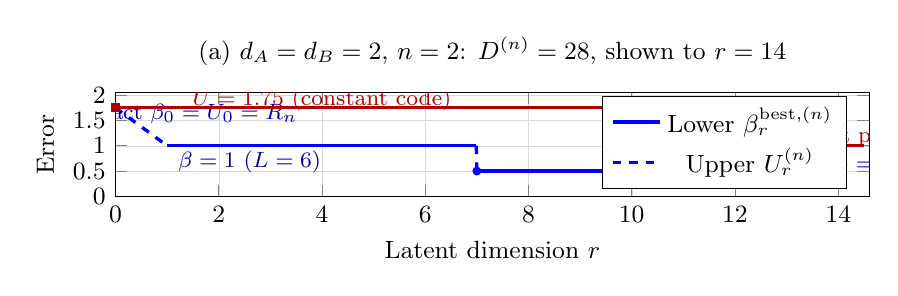
\begin{tikzpicture}
\begin{axis}[
    width=0.92\linewidth, height=2.9cm,
    xlabel={Latent dimension $r$}, ylabel={Error},
    xmin=0, xmax=14.6, ymin=0, ymax=2.05,
    xtick={0,2,4,6,8,10,12,14}, ytick={0,0.5,1,1.5,2},
    grid=both, grid style={line width=.1pt, draw=gray!30},
    legend pos=north east, legend style={font=\small},
    tick label style={font=\small}, label style={font=\small},
    title={(a) $d_A=d_B=2$, $n=2$: $D^{(n)}=28$, shown to $r=14$},
    title style={font=\small}
]
\addplot[blue, very thick] coordinates {(1,1) (6.99,1)};
\addplot[blue, very thick, dashed] coordinates {(0,1.75) (1,1)};
\addplot[blue, very thick] coordinates {(7,0.5) (12.99,0.5)};
\addplot[blue, very thick, dashed] coordinates {(6.99,1) (7,0.5)};
\addplot[blue, only marks, mark=*, mark size=1.4pt] coordinates {(0,1.75) (7,0.5)};
\node at (axis cs:1.5,1.62) [font=\footnotesize, blue!70!black] {exact $\beta_0=U_0=R_n$};
\addplot[red!70!black, very thick] coordinates {(0,1.75) (11.99,1.75)};
\addplot[red!70!black, very thick] coordinates {(12,1) (14.5,1)};
\addplot[red!70!black, very thick, dashed] coordinates {(11.99,1.75) (12,1)};
\addplot[red!70!black, only marks, mark=square*, mark size=1.4pt] coordinates {(0,1.75) (12,1)};
\node at (axis cs:9.4,0.62) [anchor=west, font=\footnotesize, blue!70!black] {$\beta=\gamma=\max\{1/4,1/2\}=1/2$};
\node at (axis cs:4.0,1.9) [font=\footnotesize, red!70!black] {$U=1.75$ (constant code)};
\node at (axis cs:12.7,1.18) [anchor=west, font=\footnotesize, red!70!black] {output pinching $r\ge12$};
\node at (axis cs:2.6,0.68) [font=\footnotesize, blue!70!black] {$\beta=1$ ($L=6$)};
\legend{Lower $\beta_r^{\mathrm{best},(n)}$, Upper $U_r^{(n)}$}
\end{axis}
\end{tikzpicture}

\medskip
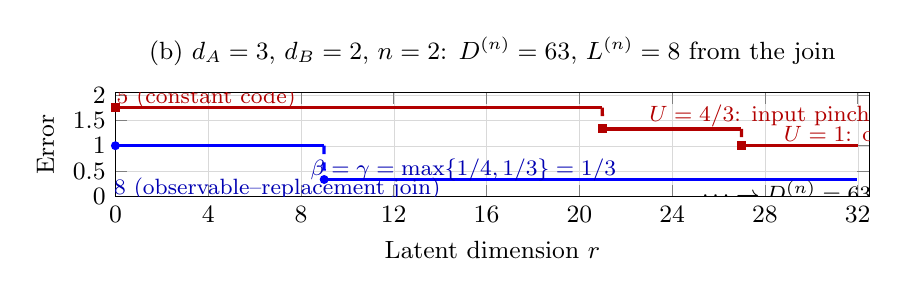
\begin{tikzpicture}
\begin{axis}[
    width=0.92\linewidth, height=2.9cm,
    xlabel={Latent dimension $r$}, ylabel={Error},
    xmin=0, xmax=32.5, ymin=0, ymax=2.05,
    xtick={0,4,8,12,16,20,24,28,32}, ytick={0,0.5,1,1.5,2},
    grid=both, grid style={line width=.1pt, draw=gray!30},
    tick label style={font=\small}, label style={font=\small},
    title={(b) $d_A=3$, $d_B=2$, $n=2$: $D^{(n)}=63$, $L^{(n)}=8$ from the join},
    title style={font=\small}
]
\addplot[blue, very thick] coordinates {(0,1) (8.99,1)};
\addplot[blue, very thick] coordinates {(9,0.333) (31.99,0.333)};
\addplot[blue, very thick, dashed] coordinates {(8.99,1) (9,0.333)};
\addplot[blue, only marks, mark=*, mark size=1.4pt] coordinates {(0,1) (9,0.333)};
\addplot[red!70!black, very thick] coordinates {(0,1.75) (20.99,1.75)};
\addplot[red!70!black, very thick] coordinates {(21,1.333) (26.99,1.333)};
\addplot[red!70!black, very thick] coordinates {(27,1) (32,1)};
\addplot[red!70!black, very thick, dashed] coordinates {(20.99,1.75) (21,1.333)};
\addplot[red!70!black, very thick, dashed] coordinates {(26.99,1.333) (27,1)};
\addplot[red!70!black, only marks, mark=square*, mark size=1.4pt] coordinates {(0,1.75) (21,1.333) (27,1)};
\node at (axis cs:3.2,0.15) [font=\footnotesize, blue!70!black] {$\beta=1$ up to $L=8$ (observable--replacement join)};
\node at (axis cs:15,0.52) [font=\footnotesize, blue!70!black] {$\beta=\gamma=\max\{1/4,1/3\}=1/3$};
\node at (axis cs:22.6,1.58) [anchor=west, font=\footnotesize, red!70!black] {$U=4/3$: input pinching $k_{\mathrm{in}}=3$, $r\ge21$};
\node at (axis cs:28.4,1.2) [anchor=west, font=\footnotesize, red!70!black] {$U=1$: output pinching $r\ge27$};
\node at (axis cs:2.2,1.95) [font=\footnotesize, red!70!black] {$U=1.75$ (constant code)};
\node at (axis cs:33.0,0.1) [anchor=east, font=\footnotesize] {$\cdots\to D^{(n)}=63$};
\end{axis}
\end{tikzpicture}

\medskip
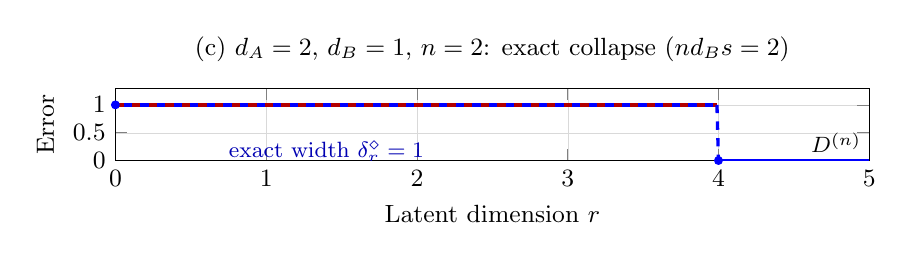
\begin{tikzpicture}
\begin{axis}[
    width=0.92\linewidth, height=2.5cm,
    xlabel={Latent dimension $r$}, ylabel={Error},
    xmin=0, xmax=5, ymin=0, ymax=1.3,
    xtick={0,1,2,3,4,5}, ytick={0,0.5,1},
    grid=both, grid style={line width=.1pt, draw=gray!30},
    tick label style={font=\small}, label style={font=\small},
    title={(c) $d_A=2$, $d_B=1$, $n=2$: exact collapse ($nd_Bs=2$)},
    title style={font=\small}
]
\addplot[blue, very thick] coordinates {(0,1) (3.99,1)};
\addplot[red!70!black, very thick, dashed] coordinates {(0,1) (3.99,1)};
\addplot[blue, very thick, dashed] coordinates {(3.99,1) (4,0)};
\addplot[blue, very thick] coordinates {(4,0) (5,0)};
\addplot[blue, only marks, mark=*, mark size=1.4pt] coordinates {(0,1) (4,0)};
\node at (axis cs:1.4,0.15) [font=\footnotesize, blue!70!black] {exact width $\delta_r^{\diamond}=1$};
\node at (axis cs:4.55,0.32) [anchor=west, font=\footnotesize] {$D^{(n)}=4$};
\end{axis}
\end{tikzpicture}
{\small\caption{Certified lower and upper envelopes of the instrument compression width. (a) The worked example $d_A=d_B=2$, $n=2$ (Example~\ref{ex:222}): the upgraded value $\beta_0=R_n=1.75$ at $r=0$ (exact, meeting the upper envelope) and $\beta_r^{\mathrm{best},(n)}=1$ for $1\le r\le6$, with $\gamma=\max\{\rho_n,1/d_A\}=1/2$ for $7\le r<28$; the upper envelope is $R_{\mathrm{inst}}=1.75$ for $0\le r<12$ and $1$ from balanced two-sector output pinching for $12\le r\le14$, while convex projection exceeds $1.75$ throughout and input pinching enters at $r_{\mathrm{in}}=14$ with the same value $1$. (b) $d_A=3$, $d_B=2$, $n=2$: the one-sphere dimension $L^{(n)}=8$ comes from the observable--replacement join; the upper envelope steps down $1.75\to4/3\to1$ at $r=21$ (three-block input pinching) and $r=27$ (two-block output pinching), and the intermediate lower bound is $\gamma=1/3$. (c) The exact collapse for $d_A=2$, $d_B=1$, $n=2$ (Theorem~\ref{thm:collapse}): both envelopes equal the exact width, which is $1$ below $D^{(n)}=4$ and $0$ from $D^{(n)}$ on. Filled circles and squares mark the lower and upper envelopes in (a) and (b); dashed segments mark the jumps.}
}
\label{fig:envelope}
\end{figure}

\begin{table}[t]
\centering
\small
\setlength{\tabcolsep}{4pt}
\begin{tabular}{p{3.4cm}p{3.0cm}p{3.0cm}p{3.4cm}}
\toprule
Quantity & Channel $n=1$ & Instrument $n\ge1$ & Origin \\
\midrule
Affine dimension & $d_A^2(d_B^2-1)$ & $d_A^2(nd_B^2-1)$ & $nd_A^2d_B^2-d_A^2$ via surjectivity of the marginal map $(X_1,\dots,X_n)\mapsto\sum_k\Tr_BX_k=H$, e.g.\ $X_1=H\otimes I_B/d_B$\\
Centred in-radius & $2/d_Bs$ & $2/nd_Bs$ & $\max\{0,\lambda_{\max}(-X)\}\le s\|\vD\|_{\diamond,\mathrm{inst}}/2d_A$, $s=\min\{d_A,d_B\}$\\
Covering radius $R(\mathcal I_*)$ & $2(1-1/d_Bs)$ & $2(1-1/nd_Bs)$ & $\sigma_{EBC_n}\le nd_Bs\,(\rho_E\otimes I_B/d_B\otimes I_{C_n}/n)$ plus $a\le Kb$\\
Replacement sphere & $S^{d_B^2-2}$ & $S^{nd_B^2-2}$ & $X\mapsto X_+/t_X$, orthogonal Jordan supports\\
Full-direction sphere & $S^{d_A^2(d_B^2-1)-1}$ & $S^{D^{(n)}-1}$ & Jordan decomposition plus correction state $\nu=(I_{A_0}-\mu)/(d_A-1)$ for $d_A\ge2$; for $d_A=1$ set $J^\pm=\Theta_\pm$\\
Diamond diameter & $2$ & $2$ & flagged channels have diamond norm $1$; orthogonal flagged states attain $2$\\
Zero-error threshold & $d_A^2(d_B^2-1)$ & $d_A^2(nd_B^2-1)$ & affine coordinates plus Borsuk--Ulam collision\\
\bottomrule
\end{tabular}
\caption{Channel versus instrument exact geometry. The $1/n$ factor is the uniform trace-budget split among $n$ outcomes at the uniform centre; the same numerical positivity budget $2/(nd_Bs)$ is realised by two distinct witnesses --- an orthogonal-output isometry witness for $d_B>1$, and an effect-transfer witness ($\pm\mathcal F/2$) for $d_B=1$, $n\ge2$ --- which live in different faces of the positive cone. Maximality of the radius uses the eigenvalue $1/(nd_Ad_B)-s\,t'/(2d_A)<0$ for $t'>t$, or $1/(nd_A)-t'/(2d_A)<0$ in the POVM case. The sphere rows are stated in the non-singleton regimes ($d_B>1$ for channels, $nd_B>1$ for instruments); the $n=d_B=1$ singleton is described in Remark~\ref{rem:degenerate}.}
\label{tab:comparison}
\end{table}

\begin{table}[t]
\centering
\small
\setlength{\tabcolsep}{4pt}
\begin{tabular}{ccccccccc}
\toprule
$(d_A,d_B,n)$ & $D^{(n)}$ & $L_{\mathrm{rep}}$ & $L_{\mathrm{obs}}$ & $N_{\mathrm{join}}$ & $L_{\mathrm{join}}$ & $L_{A,B}^{(n)}$ & $\gamma_{A,B}^{(n)}$\\
\midrule
$(2,2,2)$ & $28$ & $6$ & $2$ & $2$ & $3$ & $6$ & $1/2$\\
$(3,2,2)$ & $63$ & $6$ & $7$ & $2$ & $8$ & $8$ & $1/3$\\
$(2,3,1)$ & $32$ & $7$ & $2$ & $1$ & $2$ (degenerate) & $7$ & $1/2$\\
$(2,1,2)$ & $4$  & $0$ & $2$ & $0$ & invalid & $2$ & $1$\\
\bottomrule
\end{tabular}
\caption{Certified one-sphere dimensions and intermediate envelope value, with $L_{A,B}^{(n)}=\min\{D^{(n)}-1,\max\{L_{\mathrm{rep}},L_{\mathrm{obs}},L_{\mathrm{join}}\}\}$ and $\gamma_{A,B}^{(n)}=\max\{\rho_n,1/d_A\}$. For $(2,1,2)$ one has $nd_Bs=2$ and the collapse of Theorem~\ref{thm:collapse} applies: $\beta_r^{\mathrm{best}}=1$ throughout $r<D$.}
\label{tab:thresholds}
\end{table}

\section{Conclusion}
\label{sec:conclusion}

The exact results of this paper are the affine dimension, the centred in-radius and its global optimality, the covering radius and the diameter, the constant-code width, the zero-error threshold, the replacement profile, and the collapse case, collected in Table~\ref{tab:summary}. The structural fact behind this exactness is the concave--convex duality of the uniform instrument (Theorem~\ref{thm:global-inradius} and Remark~\ref{rem:duality}): the same object is optimal both as the centre of the largest contained ball and as the centre of the smallest covering ball. The intermediate widths, by contrast, are certified rather than exact: the lower envelope combines the two mechanisms of Remark~\ref{rem:gamma-mechanisms}, the upper envelope is attained by explicit constructions, and the bracket between them remains open in general.

The results specialise consistently. For $n=1$ they recover the channel-level theorems of Ref.~\cite{CompanionChannels}; for $d_B=1$ they govern finite-outcome measurements; and for $d_A=1$ the antipodal profile of the full body is exact, so the top subcritical width and the one-sphere values of the envelope are determined exactly, while the input-independent subcritical widths obey the coordinate dichotomy for $d_B\in\{1,2\}$ --- $\delta_r=1$ exactly above the diagonal $nd_B\le2r+2$ (classical: $n\le2r+2$; qubit: $r\ge n-1$), $\delta_r\ge4/3$ below it, with the exact boundary value $4/3$ (Corollaries~\ref{cor:classical-dichotomy}, \ref{cor:qubit-dichotomy}, \ref{cor:exact-d1}) --- and the exact value $2(1-1/d_B)$ at $r=n-1$ for prime-power output dimensions (Theorem~\ref{thm:mass-exact}); at the bottom index the classification is complete --- $\delta_1=1$ exactly on the classical $n\le4$ and qubit $n\le2$ bodies, $\delta_1\ge4/3$ on every other, with the qutrit state space exactly at $4/3$ and the ququart in $[4/3,3/2]$ (Theorems~\ref{thm:equal-basis} and~\ref{thm:state-nonflat}, Corollary~\ref{cor:bottom-dichotomy}) --- at the second index every $d_B\ge3$ state space is again bounded below by $4/3$, exactly $4/3$ at the qutrit (Theorem~\ref{thm:state-d2}, proved through the cohomology of the flag quotient; Lemma~\ref{lem:flag-cohomology} and Proposition~\ref{prop:cupsquare}) --- and the coordinate Conjecture~\ref{con:coord-flat} covering the $d_B\ge3$ flat direction at $r\ge3$, gated by the state-space widths through Lemma~\ref{lem:slice-gate}. The $1/n$ suppression of the centred radius against the $n$-fold growth of the affine dimension (Corollary~\ref{cor:scaling}) quantifies the cost of recording outcomes, and the threshold of Theorem~\ref{thm:collapse} identifies the cases in which the envelopes close.

The following problems remain open: (i) determine the intermediate widths $\delta_{r,\mathrm{inst}}^{\diamond}(A,B)$ for $L_{A,B}^{(n)}<r<D_{A,B}^{(n)}$, or improve either envelope; (ii) determine the largest index $r$ with $\alpha_r(\Inst_n(A,B))=1$; (iii) resolve the boundary cases $c=d_B^2$ and $c=d_A^2d_B^2$ of the scaling trichotomy of Corollary~\ref{cor:scaling}; (iv) determine whether the uniform instrument is the unique optimal centre for the in-radius and for the covering radius; (v) settle the coordinate flat-widths Conjecture~\ref{con:coord-flat} for $d_A=1$, $d_B\ge3$ at $r\ge3$ --- by the concentration gate of Lemma~\ref{lem:slice-gate} the gating unknowns are the state-space widths $\delta_r(\mathcal D(B))$, of which the smallest, $\delta_2$ of the qutrit, is exactly $4/3$ (Theorem~\ref{thm:state-d2}), so the first open gating unknowns are $\delta_2$ of the ququart and $\delta_3$ of the qutrit; determine the exact sub-diagonal widths, bracketed in $[2(q-1)/q,\ 2(n-2r-1)/(n-2r+2)]$ for $d_B=1$ (Theorems~\ref{thm:nonflat-d1} and~\ref{thm:tverberg}, Propositions~\ref{prop:pair-d1} and~\ref{prop:mass-split}(i)) and in $[4/3,\ 2-1/k]$ for $d_B=2$ at $r=n-k$ (Remark~\ref{rem:flat-status}); and close the one-outcome ququart, bracketed in $[4/3,\,3/2]$ (Theorem~\ref{thm:state-nonflat}); (vi) determine the unstable integral cohomology of the symmetric-group quotients themselves, where the field-coefficient algorithms of Ref.~\cite{GuerraJana2025} leave the torsion layers open --- the transgression computation of Proposition~\ref{prop:cupsquare} settles the integral cohomology of the cyclic intermediate quotient $B$, with the computational verification of Remark~\ref{rem:machine-certificate} as an independent cross-check, but neither addresses the symmetric-group quotients;

\section*{Declarations}
The author declares no funding and no competing interests. The code and computation transcripts of Remark~\ref{rem:machine-certificate} are available at the repository cited there.

\appendix

\section{Finite-program evaluation: background}
\label{app:no-programming}

This appendix records, for completeness and motivation, the no-programming obstruction for unitary channels. It is logically independent of the instrument geometry developed above: the main theorems concern \emph{representational} dimension, whereas this appendix concerns \emph{programmable evaluation} with a fixed processor.

\begin{definition}[Exact finite-program evaluator]
Let $E$ and $B$ be finite-dimensional. An exact finite-program evaluator consists of a finite-dimensional program system $M$, a completely positive trace-preserving (CPTP) processor $\Gamma:\Lin(M\otimes E)\to\Lin(B)$, and a program state $\pi_\Phi\in\Sstate(M)$ for every channel $\Phi\in\Chan(E,B)$, such that
\[
\Gamma(\pi_\Phi\otimes\rho)=\Phi(\rho)
\]
for every input state $\rho$ on $E$. By linearity the same identity holds for every input operator.
\end{definition}

\begin{theorem}[No finite exact evaluator for unitary channels]
\label{thm:no-programming}
Let $\dim E>1$. No finite-dimensional program system and fixed CPTP processor $\Gamma:\Lin(M\otimes E)\to\Lin(E)$ can exactly evaluate every unitary channel on $E$.
\end{theorem}

\begin{proof}
For pure program states, the no-programming theorem~\cite{NielsenChuang1997} shows that distinct unitary channels require orthogonal programs. It remains to pass from pure to mixed programs. Suppose
\[
\pi_U=\sum_jq_j|p_j\rangle\langle p_j|,\qquad q_j>0,
\]
is a spectral decomposition of a program that evaluates the unitary channel $\mathcal U_U$. For every pure input $|\psi\rangle$, linearity gives
\[
U|\psi\rangle\langle\psi|U^\dagger
=\sum_jq_j\,\Gamma\big(|p_j\rangle\langle p_j|\otimes|\psi\rangle\langle\psi|\big).
\]
Because $\Gamma$ is CPTP, each summand $\sigma_{j,\psi}$ is a density operator. The right-hand side is a convex decomposition of a pure state, and pure states are extreme points of the state space, so each positive-weight summand equals the same pure output: $\sigma_{j,\psi}=U|\psi\rangle\langle\psi|U^\dagger$ for all $j$ and all pure $|\psi\rangle$. Fixing $j$, the map $\Lambda_j(X)=\Gamma(|p_j\rangle\langle p_j|\otimes X)$ is a channel agreeing with $\mathcal U_U$ on every rank-one projector; rank-one projectors span $\Herm(E)$ over $\mathbb R$, and complex linearity extends the equality to all of $\Lin(E)$. Hence every unit eigenvector of $\pi_U$ with positive weight programs $\mathcal U_U$ exactly, and these eigenvectors span $\supp\pi_U$.

Applying the same argument to programs of two distinct unitary channels, the pure-state no-programming theorem makes every positive-weight eigenvector of the first program orthogonal to every positive-weight eigenvector of the second. Those eigenvectors span their respective supports, so $\supp\pi_U\perp\supp\pi_V$. A finite-dimensional program space cannot contain infinitely many mutually orthogonal nonzero supports, while $\dim E>1$ gives infinitely many distinct unitary channels. This proves the claim.
\end{proof}

\begin{corollary}[Unequal output systems]
\label{cor:unequal}
Let $\dim E>1$ and $\dim B\ge\dim E$. There is no finite-dimensional exact evaluator for all channels $E\to B$.
\end{corollary}

\begin{proof}
Choose an isometry $V:E\to B$, let $\iota(\rho)=V\rho V^\dagger$, fix a state $\omega$ on $E$, and define the recovery channel
\[
\mathcal R(\sigma)=V^\dagger\sigma V+\Tr[(I_B-VV^\dagger)\sigma]\,\omega,
\]
which is CPTP and satisfies $\mathcal R\circ\iota=\id_E$. An evaluator for all channels $E\to B$ would in particular evaluate every channel $\iota\circ\mathcal U_U$ for the fixed embedding $\iota$; postcomposing its processor with $\mathcal R$ would then give an exact finite evaluator for all unitary channels on $E$, contradicting Theorem~\ref{thm:no-programming}.
\end{proof}

\begin{corollary}[Vanishing error requires unbounded program dimension]
\label{cor:divergence}
Fix a system $E$ with $\dim E>1$. For each $j$, let $M_j$ be a program system of dimension $m_j$ and let $\Gamma_j:\Lin(M_j\otimes E)\to\Lin(E)$ be a CPTP processor. Write $\Gamma_{j,\pi}(X)=\Gamma_j(\pi\otimes X)$ and suppose
\[
\sup_{U\in\mathrm U(E)}\min_{\pi\in\Sstate(M_j)}
\|\Gamma_{j,\pi}-\mathcal U_U\|_\diamond
\le\varepsilon_j,\qquad\varepsilon_j\longrightarrow0.
\]
Then $m_j\to\infty$.
\end{corollary}

\begin{proof}
Suppose otherwise. Passing to a subsequence, assume $m_j\le m_{\max}$ for every $j$. Let $M\simeq\mathbb C^{m_{\max}}$ and choose isometries $W_j:M_j\to M$. Put $P_j=W_jW_j^\dagger$, fix $\tau_j\in\Sstate(M_j)$, and define
\[
\Lambda_j(\eta)=W_j^\dagger P_j\eta P_jW_j+\Tr[(I_M-P_j)\eta]\,\tau_j,
\]
a CPTP map $\Lin(M)\to\Lin(M_j)$: the first term is the compression onto the $P_j$-corner followed by the isometry $W_j^\dagger$, and the second is a measure-and-prepare channel on the orthocomplement (the two trace contributions add up to $\Tr\eta$). In particular $\Lambda_j(W_j\pi W_j^\dagger)=\pi$ for $\pi\in\Sstate(M_j)$. The extended processors $\widetilde\Gamma_j=\Gamma_j\circ(\Lambda_j\otimes\id_E):\Lin(M\otimes E)\to\Lin(E)$ are CPTP and preserve every originally programmed channel. The set of CPTP maps on the fixed spaces $M\otimes E\to E$ is compact, so, passing to a further subsequence \emph{chosen independently of the target unitary}, $\widetilde\Gamma_j\to\Gamma$ in diamond norm. Now fix a unitary $U$. For each $j$ choose $\pi'_j(U)\in\Sstate(M_j)$ with approximation error at most $\varepsilon_j$ (such a minimiser exists by compactness of $\Sstate(M_j)$ and continuity of the induced channel), and embed it as $\pi_j(U)=W_j\pi'_j(U)W_j^\dagger\in\Sstate(M)$. By compactness of $\Sstate(M)$ there is a $U$-dependent subsubsequence with $\pi_j(U)\to\pi_U$; along it the processors still converge to the same $\Gamma$. Continuity of the evaluation map in both processor and program state gives $\Gamma(\pi_U\otimes\cdot)=\mathcal U_U$. Since $U$ was arbitrary, the single limiting processor $\Gamma$ exactly evaluates every unitary channel, contradicting Theorem~\ref{thm:no-programming}. Hence no bounded subsequence of $(m_j)$ exists, and, $(m_j)$ being integer-valued, $m_j\to\infty$.
\end{proof}

\begin{remark}[Scope of the no-programming obstruction]
\label{rem:scope}
The result forbids a scheme that is simultaneously exact, deterministic, universal over the unitary promise class, and finite-dimensional. It does not forbid approximate, probabilistic, restricted-family, infinite-dimensional, or unbounded-register schemes, nor schemes with an externally supplied classical description. A finite classical program register is still a finite-dimensional program and is not exempt. Storing a Choi operator as a mathematical state is also distinct from evaluating the represented channel with one fixed CPTP processor. The optimal asymptotic program cost of approximate universal unitary programming is determined in~\cite{YangRennerChiribella2020}, and quantitative program-dimension lower bounds in the approximate case are obtained in~\cite{KubickiPalazuelosPerezGarcia2019}; the compactness corollary above records the qualitative divergence consequence needed for motivation. Complementary quantitative statements --- the positive finite-programming floor, program-state separation, and the packing lower bounds --- are developed in Ref.~\cite{CompanionChannels}.
\end{remark}

\section*{Data Availability}
No data were generated or analysed in this study.

\begin{thebibliography}{99}

\bibitem{Choi1975}
M.-D. Choi, \emph{Completely positive linear maps on complex matrices}, Linear Algebra Appl. \textbf{10}, 285--290 (1975).

\bibitem{CompanionChannels}
A.~Abaee, \emph{Exact diamond balls, antipodal widths, and query-uniform compression bounds for quantum channels}, submitted for publication (2026). (Submitted concurrently with the present work.)

\bibitem{Jamiolkowski1972}
A.~Jamio{\l}kowski, \emph{Linear transformations which preserve trace and positive semidefiniteness of operators}, Rep. Math. Phys. \textbf{3}, 275--278 (1972).

\bibitem{KubickiPalazuelosPerezGarcia2019}
M.~Kubicki, C. Palazuelos, and D. P\'erez-Garc\'ia, \emph{Resource quantification for the no-programing theorem}, Phys. Rev. Lett. \textbf{122}, 080505 (2019).

\bibitem{DaviesLewis1970}
E.~B. Davies and J.~T. Lewis, \emph{An operational approach to quantum probability}, Commun. Math. Phys. \textbf{17}, 239--260 (1970).

\bibitem{AharonovKitaevNisan1998}
D. Aharonov, A. Kitaev, and N. Nisan, \emph{Quantum circuits with mixed states}, in Proceedings of the Thirtieth Annual ACM Symposium on Theory of Computing (STOC 1998), ACM, New York, 1998, pp.~20--30.

\bibitem{Ozawa1984}
M. Ozawa, \emph{Quantum measuring processes of continuous observables}, J. Math. Phys. \textbf{25}, 79--87 (1984).

\bibitem{Pinkus1985}
A. Pinkus, \emph{$n$-Widths in Approximation Theory}, Ergebnisse der Mathematik und ihrer Grenzgebiete \textbf{7}, Springer, Berlin, 1985.

\bibitem{ChiribellaEtAl2009Instruments}
G. Chiribella, G.~M. D'Ariano, and P. Perinotti, \emph{Realization schemes for quantum instruments}, J. Math. Phys. \textbf{50}, 042101 (2009).

\bibitem{ChiribellaEtAl2008Combs}
G. Chiribella, G.~M. D'Ariano, and P. Perinotti, \emph{Quantum circuit architecture}, Phys. Rev. Lett. \textbf{101}, 060401 (2008).

\bibitem{Helstrom1976}
C.~W. Helstrom, \emph{Quantum Detection and Estimation Theory}, Mathematics in Science and Engineering \textbf{123}, Academic Press, New York, 1976.

\bibitem{Watrous2018}
J. Watrous, \emph{The Theory of Quantum Information}, Cambridge University Press (2018).

\bibitem{NielsenChuang1997}
M.~A. Nielsen and I.~L. Chuang, \emph{Programmable quantum gate arrays}, Phys. Rev. Lett. \textbf{79}, 321--324 (1997).

\bibitem{YangRennerChiribella2020}
Y. Yang, R. Renner, and G. Chiribella, \emph{Optimal universal programming of unitary gates}, Phys. Rev. Lett. \textbf{125}, 210501 (2020).

\bibitem{Matousek2003}
J. Matou{\v{s}}ek, \emph{Using the Borsuk--Ulam Theorem}, Springer (2003).

\bibitem{Barvinok2002}
A. Barvinok, \emph{A Course in Convexity}, Graduate Studies in Mathematics \textbf{54}, AMS (2002).

\bibitem{Ozaydin1987}
M. {\"O}zaydin, \emph{Equivariant maps for the symmetric group}, unpublished manuscript, University of Wisconsin--Madison (1987).

\bibitem{Tverberg1966}
H. Tverberg, \emph{A generalization of Radon's theorem}, J. London Math. Soc. \textbf{41}, 123--128 (1966).

\bibitem{Brown1982}
K.~S. Brown, \emph{Cohomology of Groups}, Graduate Texts in Mathematics \textbf{87}, Springer, New York, 1982.

\bibitem{MilnorStasheff1974}
J.~W. Milnor and J.~D. Stasheff, \emph{Characteristic Classes}, Annals of Mathematics Studies \textbf{76}, Princeton University Press, Princeton, 1974.

\bibitem{Fulton1997}
W. Fulton, \emph{Young Tableaux: With Applications to Representation Theory and Geometry}, London Mathematical Society Student Texts \textbf{35}, Cambridge University Press, Cambridge, 1997.

\bibitem{HatcherSS}
A. Hatcher, \emph{Spectral Sequences in Algebraic Topology}, book project,
available at the author's webpage (unpublished draft).

\bibitem{GuerraJana2025}
L. Guerra and S. Jana, \emph{Cohomology of complete unordered flag manifolds},
Trans. Amer. Math. Soc. \textbf{378}, 3507--3550 (2025).

\bibitem{GuerraJanaMaiti2025}
L. Guerra, S. Jana, and A. Maiti, \emph{The mod-2 cohomology groups of
low-dimensional unordered flag manifolds and Auerbach bases},
Topology Appl. \textbf{365}, 109279 (2025).

\bibitem{WeberWojciechowski2017}
A. Weber and M. Wojciechowski, \emph{On the Pe\l{}czy\'nski conjecture on
Auerbach bases}, Commun. Contemp. Math. \textbf{19}, 1750016 (2017).

\bibitem{KorbasLorinc2003}
J. Korba{\v s} and J. L\"orinc, \emph{The $\mathbb Z_2$-cohomology cup-length
of real flag manifolds}, Fund. Math. \textbf{178}, 143--158 (2003).

\bibitem{Matszangosz2021}
\'A.~K. Matszangosz, \emph{On the cohomology rings of real flag manifolds:
Schubert cycles}, Math. Ann. \textbf{381}, 1537--1588 (2021).

\bibitem{Singh2010}
M. Singh, \emph{A simple proof of the Borsuk--Ulam theorem for
$\mathbb Z_p$-actions}, Topology Proc. \textbf{36}, 249--253 (2010).

\bibitem{Crabb2022}
M.~C. Crabb, \emph{A Borsuk--Ulam theorem for cyclic $p$-groups},
arXiv:2211.08087 (2022).

\end{thebibliography}

\end{document}
